%% 
%% ACS project dissertation template. 
%% 
%% Currently designed for printing two-sided, but if you prefer to 
%% print single-sided just remove ",twoside,openright" from the 
%% \documentclass[] line below. 
%%
%%
%%   SMH, May 2010. 


\documentclass[a4paper,12pt,twoside,openright]{report}


%%
%% EDIT THE BELOW TO CUSTOMIZE
%%

\def\authorname{Francisco A.\ Vargas\xspace}
\def\authorcollege{Girton College\xspace}
\def\authoremail{fav25@cam.ac.uk}
\def\dissertationtitle{Machine Learning Approaches for The Empirical Schrödinger Bridge Problem}
\def\wordcount{14962}


%\usepackage[dvips]{epsfig,graphics} 
\usepackage{epsfig,graphicx,verbatim,parskip,tabularx,setspace,xspace}
\usepackage{subfigure}
\usepackage{booktabs}
\usepackage{amsfonts}
\usepackage{xcolor}
\usepackage{pdflscape}
\usepackage{url}
\usepackage{rotating}


\usepackage{pifont}% http://ctan.org/pkg/pifont
\newcommand{\cmark}{\textcolor{green}{\ding{51}}}%
\newcommand{\xmark}{\textcolor{red}{\ding{55}}}%
\newcommand{\mmark}{\textcolor{yellow}{\textbf{!}}}
\usepackage{natbib}
\usepackage{ marvosym }


\usepackage{tikz}
\usepackage{bayesnet}
\usepackage[linesnumbered, ruled]{algorithm2e}


\usepackage{amsthm}
\usepackage{amsfonts}
\usepackage{amsthm}
\usepackage{adjustbox}
\usepackage{multirow}
\usepackage{float}

%%%%% NEW MATH DEFINITIONS %%%%%

\usepackage{amsmath,amsfonts,bm}

% Mark sections of captions for referring to divisions of figures
\newcommand{\figleft}{{\em (Left)}}
\newcommand{\figcenter}{{\em (Center)}}
\newcommand{\figright}{{\em (Right)}}
\newcommand{\figtop}{{\em (Top)}}
\newcommand{\figbottom}{{\em (Bottom)}}
\newcommand{\captiona}{{\em (a)}}
\newcommand{\captionb}{{\em (b)}}
\newcommand{\captionc}{{\em (c)}}
\newcommand{\captiond}{{\em (d)}}

\newcommand{\sigalg}{{\sigma\text{-algebra}}}

% Highlight a newly defined term
\newcommand{\newterm}[1]{{\bf #1}}


% Figure reference, lower-case.
\def\figref#1{figure~\ref{#1}}
% Figure reference, capital. For start of sentence
\def\Figref#1{Figure~\ref{#1}}
\def\twofigref#1#2{figures \ref{#1} and \ref{#2}}
\def\quadfigref#1#2#3#4{figures \ref{#1}, \ref{#2}, \ref{#3} and \ref{#4}}
% Section reference, lower-case.
\def\secref#1{section~\ref{#1}}
% Section reference, capital.
\def\Secref#1{Section~\ref{#1}}
% Reference to two sections.
\def\twosecrefs#1#2{sections \ref{#1} and \ref{#2}}
% Reference to three sections.
\def\secrefs#1#2#3{sections \ref{#1}, \ref{#2} and \ref{#3}}
% Reference to an equation, lower-case.
\def\eqref#1{equation~\ref{#1}}
% Reference to an equation, upper case
\def\Eqref#1{Equation~\ref{#1}}
% A raw reference to an equation---avoid using if possible
\def\plaineqref#1{\ref{#1}}
% Reference to a chapter, lower-case.
\def\chapref#1{chapter~\ref{#1}}
% Reference to an equation, upper case.
\def\Chapref#1{Chapter~\ref{#1}}
% Reference to a range of chapters
\def\rangechapref#1#2{chapters\ref{#1}--\ref{#2}}
% Reference to an algorithm, lower-case.
\def\algref#1{algorithm~\ref{#1}}
% Reference to an algorithm, upper case.
\def\Algref#1{Algorithm~\ref{#1}}
\def\twoalgref#1#2{algorithms \ref{#1} and \ref{#2}}
\def\Twoalgref#1#2{Algorithms \ref{#1} and \ref{#2}}
% Reference to a part, lower case
\def\partref#1{part~\ref{#1}}
% Reference to a part, upper case
\def\Partref#1{Part~\ref{#1}}
\def\twopartref#1#2{parts \ref{#1} and \ref{#2}}

\def\ceil#1{\lceil #1 \rceil}
\def\floor#1{\lfloor #1 \rfloor}
\def\1{\bm{1}}
\newcommand{\train}{\mathcal{D}}
\newcommand{\valid}{\mathcal{D_{\mathrm{valid}}}}
\newcommand{\test}{\mathcal{D_{\mathrm{test}}}}

\def\eps{{\epsilon}}


% Random variables
\def\reta{{\textnormal{$\eta$}}}
\def\ra{{\textnormal{a}}}
\def\rb{{\textnormal{b}}}
\def\rc{{\textnormal{c}}}
\def\rd{{\textnormal{d}}}
\def\re{{\textnormal{e}}}
\def\rf{{\textnormal{f}}}
\def\rg{{\textnormal{g}}}
\def\rh{{\textnormal{h}}}
\def\ri{{\textnormal{i}}}
\def\rj{{\textnormal{j}}}
\def\rk{{\textnormal{k}}}
\def\rl{{\textnormal{l}}}
% rm is already a command, just don't name any random variables m
\def\rn{{\textnormal{n}}}
\def\ro{{\textnormal{o}}}
\def\rp{{\textnormal{p}}}
\def\rq{{\textnormal{q}}}
\def\rr{{\textnormal{r}}}
\def\rs{{\textnormal{s}}}
\def\rt{{\textnormal{t}}}
\def\ru{{\textnormal{u}}}
\def\rv{{\textnormal{v}}}
\def\rw{{\textnormal{w}}}
\def\rx{{\textnormal{x}}}
\def\ry{{\textnormal{y}}}
\def\rz{{\textnormal{z}}}

% Random vectors
\def\rvepsilon{{\mathbf{\epsilon}}}
\def\rvtheta{{\mathbf{\theta}}}
\def\rva{{\mathbf{a}}}
\def\rvb{{\mathbf{b}}}
\def\rvc{{\mathbf{c}}}
\def\rvd{{\mathbf{d}}}
\def\rve{{\mathbf{e}}}
\def\rvf{{\mathbf{f}}}
\def\rvg{{\mathbf{g}}}
\def\rvh{{\mathbf{h}}}
\def\rvu{{\mathbf{i}}}
\def\rvj{{\mathbf{j}}}
\def\rvk{{\mathbf{k}}}
\def\rvl{{\mathbf{l}}}
\def\rvm{{\mathbf{m}}}
\def\rvn{{\mathbf{n}}}
\def\rvo{{\mathbf{o}}}
\def\rvp{{\mathbf{p}}}
\def\rvq{{\mathbf{q}}}
\def\rvr{{\mathbf{r}}}
\def\rvs{{\mathbf{s}}}
\def\rvt{{\mathbf{t}}}
\def\rvu{{\mathbf{u}}}
\def\rvv{{\mathbf{v}}}
\def\rvw{{\bm{\beta}}}
\def\rvx{{\mathbf{x}}}
\def\rvy{{\mathbf{y}}}
\def\rvz{{\mathbf{z}}}
\def\rvsigma{{\bm{\sigma}}}
\def\rvepsilon{{\bm{\epsilon}}}

% Elements of random vectors
\def\erva{{\textnormal{a}}}
\def\ervb{{\textnormal{b}}}
\def\ervc{{\textnormal{c}}}
\def\ervd{{\textnormal{d}}}
\def\erve{{\textnormal{e}}}
\def\ervf{{\textnormal{f}}}
\def\ervg{{\textnormal{g}}}
\def\ervh{{\textnormal{h}}}
\def\ervi{{\textnormal{i}}}
\def\ervj{{\textnormal{j}}}
\def\ervk{{\textnormal{k}}}
\def\ervl{{\textnormal{l}}}
\def\ervm{{\textnormal{m}}}
\def\ervn{{\textnormal{n}}}
\def\ervo{{\textnormal{o}}}
\def\ervp{{\textnormal{p}}}
\def\ervq{{\textnormal{q}}}
\def\ervr{{\textnormal{r}}}
\def\ervs{{\textnormal{s}}}
\def\ervt{{\textnormal{t}}}
\def\ervu{{\textnormal{u}}}
\def\ervv{{\textnormal{v}}}
\def\ervw{{\textnormal{w}}}
\def\ervx{{\textnormal{x}}}
\def\ervy{{\textnormal{y}}}
\def\ervz{{\textnormal{z}}}

% Random matrices
\def\rmA{{\mathbf{A}}}
\def\rmB{{\mathbf{B}}}
\def\rmC{{\mathbf{C}}}
\def\rmD{{\mathbf{D}}}
\def\rmE{{\mathbf{E}}}
\def\rmF{{\mathbf{F}}}
\def\rmG{{\mathbf{G}}}
\def\rmH{{\mathbf{H}}}
\def\rmI{{\mathbf{I}}}
\def\rmJ{{\mathbf{J}}}
\def\rmK{{\mathbf{K}}}
\def\rmL{{\mathbf{L}}}
\def\rmM{{\mathbf{M}}}
\def\rmN{{\mathbf{N}}}
\def\rmO{{\mathbf{O}}}
\def\rmP{{\mathbf{P}}}
\def\rmQ{{\mathbf{Q}}}
\def\rmR{{\mathbf{R}}}
\def\rmS{{\mathbf{S}}}
\def\rmT{{\mathbf{T}}}
\def\rmU{{\mathbf{U}}}
\def\rmV{{\mathbf{V}}}
\def\rmW{{\mathbf{W}}}
\def\rmX{{\mathbf{X}}}
\def\rmY{{\mathbf{Y}}}
\def\rmZ{{\mathbf{Z}}}

% Elements of random matrices
\def\ermA{{\textnormal{A}}}
\def\ermB{{\textnormal{B}}}
\def\ermC{{\textnormal{C}}}
\def\ermD{{\textnormal{D}}}
\def\ermE{{\textnormal{E}}}
\def\ermF{{\textnormal{F}}}
\def\ermG{{\textnormal{G}}}
\def\ermH{{\textnormal{H}}}
\def\ermI{{\textnormal{I}}}
\def\ermJ{{\textnormal{J}}}
\def\ermK{{\textnormal{K}}}
\def\ermL{{\textnormal{L}}}
\def\ermM{{\textnormal{M}}}
\def\ermN{{\textnormal{N}}}
\def\ermO{{\textnormal{O}}}
\def\ermP{{\textnormal{P}}}
\def\ermQ{{\textnormal{Q}}}
\def\ermR{{\textnormal{R}}}
\def\ermS{{\textnormal{S}}}
\def\ermT{{\textnormal{T}}}
\def\ermU{{\textnormal{U}}}
\def\ermV{{\textnormal{V}}}
\def\ermW{{\textnormal{W}}}
\def\ermX{{\textnormal{X}}}
\def\ermY{{\textnormal{Y}}}
\def\ermZ{{\textnormal{Z}}}

% Vectors
\def\vzero{{\bm{0}}}
\def\vone{{\bm{1}}}
\def\vmu{{\bm{\mu}}}
\def\vtheta{{\bm{\theta}}}
\def\vlambda{{\bm{\lambda}}}
\def\va{{\bm{a}}}
\def\vb{{\bm{b}}}
\def\vc{{\bm{c}}}
\def\vd{{\bm{d}}}
\def\ve{{\bm{e}}}
\def\vf{{\bm{f}}}
\def\vg{{\bm{g}}}
\def\vh{{\bm{h}}}
\def\vi{{\bm{i}}}
\def\vj{{\bm{j}}}
\def\vk{{\bm{k}}}
\def\vl{{\bm{l}}}
\def\vm{{\bm{m}}}
\def\vn{{\bm{n}}}
\def\vo{{\bm{o}}}
\def\vp{{\bm{p}}}
\def\vq{{\bm{q}}}
\def\vr{{\bm{r}}}
\def\vs{{\bm{s}}}
\def\vt{{\bm{t}}}
\def\vu{{\bm{u}}}
\def\vv{{\bm{v}}}
\def\vw{{\bm{w}}}
\def\vx{{\bm{x}}}
\def\vy{{\bm{y}}}
\def\vz{{\bm{z}}}

% Elements of vectors
\def\evalpha{{\alpha}}
\def\evbeta{{\beta}}
\def\evepsilon{{\epsilon}}
\def\evlambda{{\lambda}}
\def\evomega{{\omega}}
\def\evmu{{\mu}}
\def\evpsi{{\psi}}
\def\evsigma{{\sigma}}
\def\evtheta{{\theta}}
\def\eva{{a}}
\def\evb{{b}}
\def\evc{{c}}
\def\evd{{d}}
\def\eve{{e}}
\def\evf{{f}}
\def\evg{{g}}
\def\evh{{h}}
\def\evi{{i}}
\def\evj{{j}}
\def\evk{{k}}
\def\evl{{l}}
\def\evm{{m}}
\def\evn{{n}}
\def\evo{{o}}
\def\evp{{p}}
\def\evq{{q}}
\def\evr{{r}}
\def\evs{{s}}
\def\evt{{t}}
\def\evu{{u}}
\def\evv{{v}}
\def\evw{{w}}
\def\evx{{x}}
\def\evy{{y}}
\def\evz{{z}}

% Matrix
\def\mA{{\bm{A}}}
\def\mB{{\bm{B}}}
\def\mC{{\bm{C}}}
\def\mD{{\bm{D}}}
\def\mE{{\bm{E}}}
\def\mF{{\bm{F}}}
\def\mG{{\bm{G}}}
\def\mH{{\bm{H}}}
\def\mI{{\bm{I}}}
\def\mJ{{\bm{J}}}
\def\mK{{\bm{K}}}
\def\mL{{\bm{L}}}
\def\mM{{\bm{M}}}
\def\mN{{\bm{N}}}
\def\mO{{\bm{O}}}
\def\mP{{\bm{P}}}
\def\mQ{{\bm{Q}}}
\def\mR{{\bm{R}}}
\def\mS{{\bm{S}}}
\def\mT{{\bm{T}}}
\def\mU{{\bm{U}}}
\def\mV{{\bm{V}}}
\def\mW{{\bm{W}}}
\def\mX{{\bm{X}}}
\def\mY{{\bm{Y}}}
\def\mZ{{\bm{Z}}}
\def\mBeta{{\bm{\beta}}}
\def\mPhi{{\bm{\Phi}}}
\def\mLambda{{\bm{\Lambda}}}
\def\mSigma{{\bm{\Sigma}}}

% Tensor
\DeclareMathAlphabet{\mathsfit}{\encodingdefault}{\sfdefault}{m}{sl}
\SetMathAlphabet{\mathsfit}{bold}{\encodingdefault}{\sfdefault}{bx}{n}
\newcommand{\tens}[1]{\bm{\mathsfit{#1}}}
\def\tA{{\tens{A}}}
\def\tB{{\tens{B}}}
\def\tC{{\tens{C}}}
\def\tD{{\tens{D}}}
\def\tE{{\tens{E}}}
\def\tF{{\tens{F}}}
\def\tG{{\tens{G}}}
\def\tH{{\tens{H}}}
\def\tI{{\tens{I}}}
\def\tJ{{\tens{J}}}
\def\tK{{\tens{K}}}
\def\tL{{\tens{L}}}
\def\tM{{\tens{M}}}
\def\tN{{\tens{N}}}
\def\tO{{\tens{O}}}
\def\tP{{\tens{P}}}
\def\tQ{{\tens{Q}}}
\def\tR{{\tens{R}}}
\def\tS{{\tens{S}}}
\def\tT{{\tens{T}}}
\def\tU{{\tens{U}}}
\def\tV{{\tens{V}}}
\def\tW{{\tens{W}}}
\def\tX{{\tens{X}}}
\def\tY{{\tens{Y}}}
\def\tYQ{{\tens{{\:}_q\!Y}}}
\def\tZ{{\tens{Z}}}


% Graph
\def\gA{{\mathcal{A}}}
\def\gB{{\mathcal{B}}}
\def\gC{{\mathcal{C}}}
\def\gD{{\mathcal{D}}}
\def\gE{{\mathcal{E}}}
\def\gF{{\mathcal{F}}}
\def\gG{{\mathcal{G}}}
\def\gH{{\mathcal{H}}}
\def\gI{{\mathcal{I}}}
\def\gJ{{\mathcal{J}}}
\def\gK{{\mathcal{K}}}
\def\gL{{\mathcal{L}}}
\def\gM{{\mathcal{M}}}
\def\gN{{\mathcal{N}}}
\def\gO{{\mathcal{O}}}
\def\gP{{\mathcal{P}}}
\def\gQ{{\mathcal{Q}}}
\def\gR{{\mathcal{R}}}
\def\gS{{\mathcal{S}}}
\def\gT{{\mathcal{T}}}
\def\gU{{\mathcal{U}}}
\def\gV{{\mathcal{V}}}
\def\gW{{\mathcal{W}}}
\def\gX{{\mathcal{X}}}
\def\gY{{\mathcal{Y}}}
\def\gZ{{\mathcal{Z}}}

% Sets
\def\sA{{\mathbb{A}}}
\def\sB{{\mathbb{B}}}
\def\sC{{\mathbb{C}}}
\def\sD{{\mathbb{D}}}
% Don't use a set called E, because this would be the same as our symbol
% for expectation.
\def\sF{{\mathbb{F}}}
\def\sG{{\mathbb{G}}}
\def\sH{{\mathbb{H}}}
\def\sI{{\mathbb{I}}}
\def\sJ{{\mathbb{J}}}
\def\sK{{\mathbb{K}}}
\def\sL{{\mathbb{L}}}
\def\sM{{\mathbb{M}}}
\def\sN{{\mathbb{N}}}
\def\sO{{\mathbb{O}}}
\def\sP{{\mathbb{P}}}
\def\sQ{{\mathbb{Q}}}
\def\sR{{\mathbb{R}}}
\def\sS{{\mathbb{S}}}
\def\sT{{\mathbb{T}}}
\def\sU{{\mathbb{U}}}
\def\sV{{\mathbb{V}}}
\def\sW{{\mathbb{W}}}
\def\sX{{\mathbb{X}}}
\def\sY{{\mathbb{Y}}}
\def\sZ{{\mathbb{Z}}}

% Entries of a matrix
\def\emLambda{{\Lambda}}
\def\emA{{A}}
\def\emB{{B}}
\def\emC{{C}}
\def\emD{{D}}
\def\emE{{E}}
\def\emF{{F}}
\def\emG{{G}}
\def\emH{{H}}
\def\emI{{I}}
\def\emJ{{J}}
\def\emK{{K}}
\def\emL{{L}}
\def\emM{{M}}
\def\emN{{N}}
\def\emO{{O}}
\def\emP{{P}}
\def\emQ{{Q}}
\def\emR{{R}}
\def\emS{{S}}
\def\emT{{T}}
\def\emU{{U}}
\def\emV{{V}}
\def\emW{{W}}
\def\emX{{X}}
\def\emY{{Y}}
\def\emZ{{Z}}
\def\emSigma{{\Sigma}}

% entries of a tensor
% Same font as tensor, without \bm wrapper
\newcommand{\etens}[1]{\mathsfit{#1}}
\def\etLambda{{\etens{\Lambda}}}
\def\etA{{\etens{A}}}
\def\etB{{\etens{B}}}
\def\etC{{\etens{C}}}
\def\etD{{\etens{D}}}
\def\etE{{\etens{E}}}
\def\etF{{\etens{F}}}
\def\etG{{\etens{G}}}
\def\etH{{\etens{H}}}
\def\etI{{\etens{I}}}
\def\etJ{{\etens{J}}}
\def\etK{{\etens{K}}}
\def\etL{{\etens{L}}}
\def\etM{{\etens{M}}}
\def\etN{{\etens{N}}}
\def\etO{{\etens{O}}}
\def\etP{{\etens{P}}}
\def\etQ{{\etens{Q}}}
\def\etR{{\etens{R}}}
\def\etS{{\etens{S}}}
\def\etT{{\etens{T}}}
\def\etU{{\etens{U}}}
\def\etV{{\etens{V}}}
\def\etW{{\etens{W}}}
\def\etX{{\etens{X}}}
\def\etY{{\etens{Y}}}
\def\etZ{{\etens{Z}}}


\def\uni{{\text{Uniform}}}
\def\gam{{\text{Gamma}}}
\def\erf{{\text{erf}}}
\def\sigms{{\text{sigmoid}}}
% \def\softplus{{\text{softplus}}}
\def\logit{{\text{logit}}}
\def\bdist{{\text{Beta}}}
\def\dir{{\text{Dir}}}
\def\cat{{\text{Cat}}}
\def\bern{{\text{Bernoulli}}}
\def\NN{{\text{NN}}}
\def\yset{{\{y_i\}}}
\def\xset{{\{\vx_i\}}}
\def\tset{{\{\theta_i\}}}
\def\uchi{{\Phi_{\vx_i, \vlambda}^{-1}(u)}}
\def\uchic{{\Phi_{\vx_i, \vlambda,c}^{-1}(u)}}
\def\uchj{{\Phi_{\vx_j, \vlambda}^{-1}(u)}}
\def\uchkij{{\Phi_{\vx_i, \vlambda}^{-1}(\Phi_{\vx_j, \vlambda}(v))}}
\def\uchkijt{{\Phi_{\vx_i, \vlambda}^{-1}(\Phi_{\vx_j, \vlambda}(\theta_j))}}
\def\uch{{\Phi_{\vx^*, \vlambda}^{-1}(u)}}
\def\uchis{{\Phi_{\vx_i, \vlambda}^{-1}(u_{(s)})}}
\def\uchih{{\Phi_{\vx_i, \hat{\vlambda}}^{-1}(u)}}
\def\uchh{{\Phi_{\vx^*, \hat{\vlambda} }^{-1}(u)}}

% \def\logsumexp{{\text{logsumexp}}}

% The true underlying data generating distribution
\newcommand{\pdata}{p_{\rm{data}}}
% The empirical distribution defined by the training set
\newcommand{\ptrain}{\hat{p}_{\rm{data}}}
\newcommand{\Ptrain}{\hat{P}_{\rm{data}}}
% The model distribution
\newcommand{\pmodel}{p_{\rm{model}}}
\newcommand{\Pmodel}{P_{\rm{model}}}
\newcommand{\ptildemodel}{\tilde{p}_{\rm{model}}}
% Stochastic autoencoder distributions
\newcommand{\pencode}{p_{\rm{encoder}}}
\newcommand{\pdecode}{p_{\rm{decoder}}}
\newcommand{\precons}{p_{\rm{reconstruct}}}

\newcommand{\laplace}{\mathrm{Laplace}} % Laplace distribution

\newcommand{\E}{\mathbb{E}}
\newcommand{\W}{\mathbb{W}}
\newcommand{\Ls}{\mathcal{L}}
\newcommand{\R}{\mathbb{R}}
\newcommand{\emp}{\tilde{p}}
\newcommand{\lr}{\alpha}
\newcommand{\reg}{\lambda}
\newcommand{\rect}{\mathrm{rectifier}}
\newcommand{\softmax}{\mathrm{softmax}}
\newcommand{\sigmoid}{\sigma}
\newcommand{\softplus}{{\text{softplus}}}

\def\calP{{\mathcal{P}}}
\def\calD{{\mathcal{D}}}
\def\calF{{\mathcal{F}}}
\def\calQ{{\mathcal{Q}}}
\def\calB{{\mathcal{B}}}
\def\calN{{\mathcal{N}}}
\def\calL{{\mathcal{L}}}
\def\callambda{{\mathcal{\lambda}}}
\def\calW{{\mathcal{W}}}
\def\calT{{\mathcal{T}}}

\def\calH{{\mathcal{H}}}


\let\log\relax
\DeclareMathOperator{\log}{ln}

\def\P{{\mathbb{P}}}
\def\F{{\mathbb{F}}}
\def\Q{{\mathbb{Q}}}
\def\B{{\mathbb{B}}}
\def\I{{\mathbb{I}_d}}
\def\ind{{\bm{1}}}
\def\R{{\mathbb{R}}}
\def\X{{\mathbb{X}}}


\def\hphi{{\hat{\phi}}}


% \def\KL{{D_{\text{KL}}}}

\newcommand{\indep}{\raisebox{0.05em}{\rotatebox[origin=c]{90}{$\models$}}}


\newcommand\independent{\protect\mathpalette{\protect\independenT}{\perp}}
\def\independenT#1#2{\mathrel{\rlap{$#1#2$}\mkern2mu{#1#2}}}

\def\probspace{{(\Omega, \mathcal{F}, \mathbb{P})}}
\def\filtprobspace{{(\Omega, \mathcal{F}, \mathfrak{F}, \mathbb{P})}}

\newcommand{\KL}{D_{\mathrm{KL}}}
\newcommand{\Var}{\mathrm{Var}}
\newcommand{\standarderror}{\mathrm{SE}}
\newcommand{\Cov}{\mathrm{Cov}}
% Wolfram Mathworld says $L^2$ is for function spaces and $\ell^2$ is for vectors
% But then they seem to use $L^2$ for vectors throughout the site, and so does
% wikipedia.
\newcommand{\normlzero}{L^0}
\newcommand{\normlone}{L^1}
\newcommand{\normltwo}{L^2}
\newcommand{\normlp}{L^p}
\newcommand{\normmax}{L^\infty}

\def\vec{{\text{vec}}}

\newcommand{\parents}{Pa} % See usage in notation.tex. Chosen to match Daphne's book.

\DeclareMathOperator*{\argmax}{arg\,max}
\DeclareMathOperator*{\argmin}{arg\,min}
\DeclareMathOperator*{\arginf}{arg\,inf}
\DeclareMathOperator*{\argsup}{arg\,sup}
\DeclareMathOperator*{\logsumexp}{logsumexp}

\def\kk{{\text{k}}}

\DeclareMathOperator{\sign}{sign}
\DeclareMathOperator{\Tr}{Tr}
\let\ab\allowbreak


\newtheorem{theorem}{Theorem}
\newtheorem{lemma}{Lemma}
\newtheorem{proposition}{Proposition}

\newtheorem{observation}{Observation}
\theoremstyle{definition}
\newtheorem{definition}{Definition}[section]

\makeatletter
\def\mathcolor#1#{\@mathcolor{#1}}
\def\@mathcolor#1#2#3{%
  \protect\leavevmode
  \begingroup
    \color#1{#2}#3%
  \endgroup
}
\makeatother

%TC:ignore
\newcolumntype{L}{@{}l}
\newcolumntype{F}{l@{}}
\newcolumntype{C}{c@{}}
%TC:endignore


%% START OF DOCUMENT
\begin{document}


%% FRONTMATTER (TITLE PAGE, DECLARATION, ABSTRACT, ETC) 
\pagestyle{empty}
\singlespacing
% title page information
\begin{titlepage} 

\begin{center}
\noindent
\huge
\dissertationtitle \\
\vspace*{\stretch{1}}
\end{center}

\begin{center}
\noindent
\huge
\authorname \\
\Large
\authorcollege      \\[24pt]
%\begin{figure}

\includegraphics{CUni3.pdf}
%\end{figure}
\end{center}

\vspace{24pt} 

\begin{center}
\noindent
\large
{\it A dissertation submitted to the University of Cambridge \\ 
in partial fulfilment of the requirements for the degree of \\ 
Master of Philosophy in Advanced Computer Science} 
\vspace*{\stretch{1}}
\end{center}

\begin{center}
\noindent
University of Cambridge \\
Computer Laboratory     \\
William Gates Building  \\
15 JJ Thomson Avenue    \\
Cambridge CB3 0FD       \\
{\sc United Kingdom}    \\
\end{center}

\begin{center}
\noindent
Email: \authoremail \\
\end{center}

\begin{center}
\noindent
\today
\end{center}

\end{titlepage} 

\newpage
\vspace*{\fill}

\onehalfspacing
\newpage
%TC:ignore
{\Huge \bf Declaration}

\vspace{24pt} 

I \authorname of \authorcollege, being a candidate for the M.Phil in
Advanced Computer Science, hereby declare that this report and the
work described in it are my own work, unaided except as may be
specified below, and that the report does not contain material that
has already been used to any substantial extent for a comparable
purpose.

\vspace{24pt}
Total word count: \wordcount

\vspace{60pt}
\textbf{Signed}: 

\vspace{12pt}
\textbf{Date}:


\vfill

This dissertation is copyright \copyright 2020 \authorname. 
\\
All trademarks used in this dissertation are hereby acknowledged.



\newpage
\vspace*{\fill}
%TC:endignore
\newpage
%TC:ignore
{\Huge \bf Acknowledgements}
\vspace{24pt} 


Ramona is the best.

\newpage
\vspace*{\fill}
%TC:endignore
\singlespacing
\newpage
{\Huge \bf Abstract}
\vspace{24pt} 


The Schrödinger bridge problem is concerned with finding the most likely stochastic evolution between two probability distributions given a prior/reference stochastic evolution. This problem was posed by Schrödinger in \cite{schrodinger1931uber,schrodinger1932theorie} and solved to a large extent. Problems of this kind, whilst not popular in the machine learning community, have direct applications such as Domain Adaptation, Hypothesis Testing, Semantic Similarity, and others.

Thus, the focus of this thesis is to carry out a preliminary study on computational approaches for estimating the Schrödinger bridge between two distributions, when these distributions are available (or can be available) through samples, as most problems in Machine Learning are.

Due to the mathematical nature of the problem, this manuscript is partly concerned with restating and re-deriving many theorems and results that are either overlooked within the mathematical community or hidden in type-written textbooks behind paywalls. Part of the aim of this sub-goal is to make the mathematical toolery behind these approaches more accessible to a broader scientific and engineering audience.

\newpage
\vspace*{\fill}


\pagenumbering{roman}
\setcounter{page}{0}
\pagestyle{plain}
\tableofcontents
%TC:ignore
\listoffigures
\listoftables
%TC:endignore
\onehalfspacing

%% START OF MAIN TEXT 

 \chapter{Introduction}
 \pagenumbering{arabic} 
 
 The motion of small particles in a fluid and the value of financial instruments as a function of time have an interesting intersection. These two processes have a large number of underlying factors (e.g.\ physical forces) that impact their trajectories and constantly change as a function of time. This constant stream of varying forces causes the trajectory of these systems to seem random and makes it infeasible to model with non-probabilistic approach. 
 
 What we call Brownian motion today is a random process. It is one of the simplest physical models used to describe the motion of small particles in a fluid. The earliest mathematical formulations of this process date back to \cite{einstein1905motion}, where the diffusion-based formulation of Brownian motion was used to describe the motion of pollen particles in a fluid. Many day-to-day processes have an element of Brownian motion within them, thus Brownian motion has become a fundamental mathematical tool when describing the motion of stochastic temporal processes.
 
 A class of Brownian-motion-driven processes that is of particular interest to many areas of applied science is the drift-augmented Brownian motion. In simple terms, this family of processes can be split into two components: a Brownian-motion-driven term and a drift which provides a directional drive to the system, much like a driving force. A particular example process that is popular in the machine learning and computational neuroscience communities is the Ornstein–Uhlenbeck (OU) process \citep{doob1942brownian}. The OU-process is used to model particles undergoing Brownian motion that are subject to friction represented by the drift term. An interesting remark is that the discrete-time analogue of the OU-process is the auto-regressive process of order $1$ -- $\text{AR}(1)$.
 
 This project is concerned with a specific event regarding Brownian-motion-driven processes proposed by Schrödinger \citep{schrodinger1931uber, schrodinger1932theorie}. The event postulates a group of particles undergoing Brownian motion in $\R^d$, where we observe their position distributions $\pi_0(\vx)$ at time $0$, and then $\pi_1(\vy)$ at time $1$. Then, consider the case where $\pi_1(\vy)$ differs significantly from the predicted distribution by Brownian motion, that is
 \begin{align*}
     \pi_1(\vy) \neq \int p(\vx, 0, \vy , 1) \pi_1(\vx) d\vx,
 \end{align*}
 where $p(\vx, 0, \vy , 1) = p(\vy_1| \vx_0)$ represents the transition density under the Brownian motion. The transition density is the probability of transitioning from $\vx$ at time $0$ to $\vy$ at time $1$. We can model this event as if the particles at time $0$ were transported to time $1$ in an unlikely manner (a rare event). Out of the many unlikely ways in which this event could have happened, the Schrödinger bridge tells us which one is the most likely. This question turns out to be equivalent to finding a drift-augmented Brownian motion that satisfies the observed distributions and is as close to Brownian motion as possible in an information-theoretic sense.
 
 Rephrasing this in a more machine-learning setting, the Schrödinger bridge is concerned with finding the most likely stochastic process that evolves a distribution $\pi_0(\vx)$ to another distribution $\pi_1(\vy)$, and is in line with a pre-specified Brownian-motion prior.
 
 From an application viewpoint, the Schrödinger bridge provides us with a theoretically-grounded mechanism for mapping between two distributions. When those distributions are only available through samples, we effectively have a classical, unsupervised domain-adaptation problem, as illustrated in Figure \ref{fig:intuitive_bridge}. Furthermore, the Schrödinger bridge also provides us with the probability of this stochastic evolution, thus allowing us to compare two data sets/distributions which can be useful for hypothesis testing \citep{gretton2012kernel,ramdas2017wasserstein} and semantic similarity \citep{vargas2019model}.
 
 In this project, we explore machine-learning-based approaches to estimating the Schrödinger bridge between two distributions that are available through samples.
\begin{figure}
    \centering
    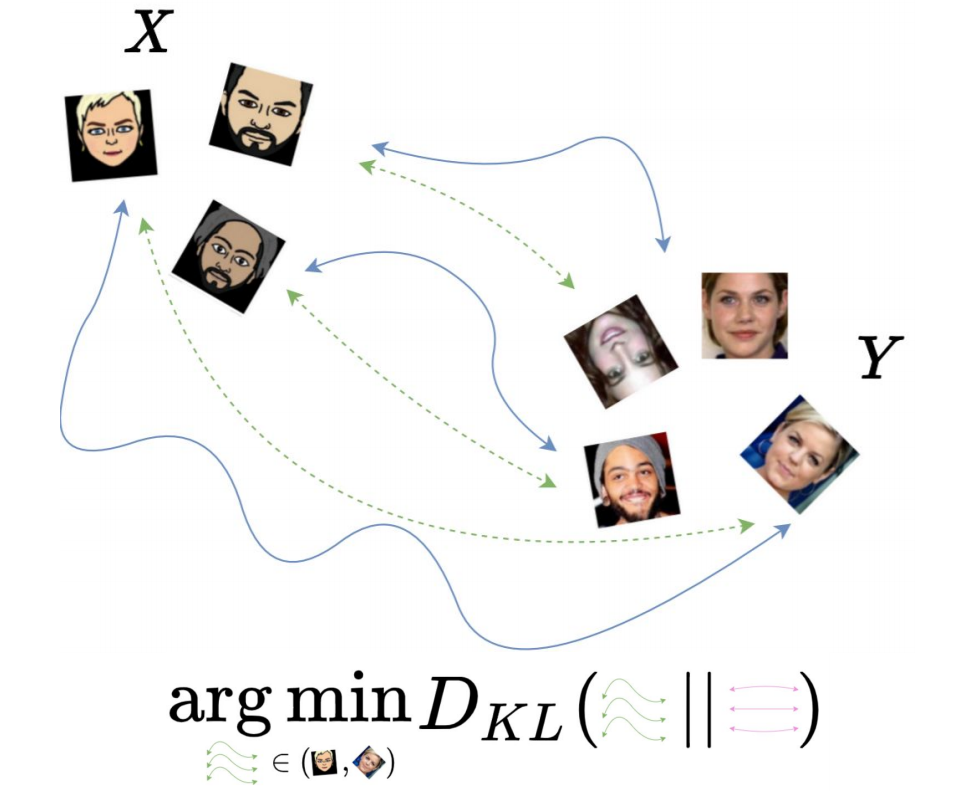
\includegraphics[scale=0.7]{images/charicaturistic_bridge.PNG}
    \caption{Intuitive Illustration of the Schrödinger Bridge}
    \label{fig:intuitive_bridge}
\end{figure}

 
\chapter{Mathematical Preliminaries}

% \setcounter{page}{1}

The goal of this chapter is to introduce mathematical notation, concepts and lemmas that we will use throughout this thesis. Whilst many of these lemmas are omitted or taken for granted in the stochastic process literature, we found that some of them were not directly accessible when searched for and not taught in graduate-level measure--- and probability-theory courses \citep{ethmeasure,mitmeasure,cambprob}. Therefore, it will be useful to restate and rederive some of these results, in order to make the theory behind Schrödinger bridges more accessible to the computational sciences.

Due to limitations of the Riemann integral, we will be briefly covering a measure-theoretic introduction to probability in order to have the background required to introduce the  Lebesgue–Stieltjes integral, which we will be using to express some of the expectations in this thesis. Furthermore, we will also be providing a sketch proof of standard results for decompositions of the Radon-Nikodym derivative which we will employ in decomposing the Kullback–Leibler (KL) divergence. 

\section{Probability Space Formalism}

For many of the technical derivations in the methodology we will study, a basic notion of measure and integration is required, thus we will refresh concepts such as $\sigalg$, probability measures,  measurable functions and the Lebesgue–Stieltjes integral, without going into unnecessary technical detail.

\begin{definition} \label{def:prob_space}
A probability space is defined as a 3-element tuple $\probspace$, where:
\begin{itemize}
    \item $\Omega$ is the sample space, i.e. the set of possible outcomes. For example, for a coin toss $\Omega=\{\text{Head}, \text{Tails}\}$. 
    \item The $\sigalg$ $\mathcal{F} \subseteq 2^{\Omega}$ represents the set of events we may want to consider. Continuing the coin toss example, we may have $\Omega=\{\emptyset, \text{Head}, \text{Tails},\{\text{Head}, \text{Tails}\}\}$.
    \item A probability measure $\P:\calF \rightarrow [0,1]$ is a function which assigns a number in $[0,1]$ to any event (set) in the $\sigalg$ $\calF$. The function $\P$ has the following requirements:
    \begin{itemize}
        \item $\sigma$-additive, which means that if  $\bigcup_{i=0}^\infty  A_i\in \calF$ and $A_j \cap A_j = \emptyset, \; i \neq j$, then $\P\left(\bigcup_{i=0}^\infty A_i\right) =\sum_{i=0}^\infty \P(A_i) $.
        \item $\P(\Omega)=1$, which we can read as the sample space summing up to (integrating) to 1.  Without this condition $\P$ would be a regular measure.
    \end{itemize}
\end{itemize}
\end{definition}
Note that we want to be able to measure (assign a probability to) each set in $\calF$ rather than $2^\Omega$, since the latter is not always possible. In other words, one can construct sets that cannot be measured (or can only be measured by the trivial measure $\callambda(A) = 0,\:\forall A \subseteq \Omega$, which is not a probability measure). Thus, we require $\calF$ to only contain measurable sets and this is what a $\sigalg$ guarantees.
\begin{definition}\label{def:sigma_algebra}
A $\sigalg$ $\calF \subseteq 2^{\Omega}$ is a collection of sets satisfying the property:
\begin{itemize}
    \item $\calF$ contains $\Omega$: $\Omega \in \calF$.
    \item $\calF$ is closed under complements: if $A\in\calF$, then $\Omega \setminus A \in \calF$.
    \item $\calF$ is closed under countable union:  if $A_i \in \calF \ \forall i$, then $\bigcup_i A_i \in \calF$.
\end{itemize}
\end{definition}

Note we use the notation $\calB(\R^d)$ for the Borel $\sigma$-algebra of $\R^d$, which we can think of as the canonical $\sigma$-algebra for $\R^d$ --- it is the most compact representation of all measurable sets in $\R^d$. This notation can also be extended for subsets of $\R^d$ and more generally to any topological space.

\begin{definition}\label{def:random_variable}
For a probability space $\probspace$, a real-valued random variable (vector) $\rvx(\omega)$ is a function $\rvx:\Omega \rightarrow \R^d$, requiring that $\rvx(\omega)$ is a measurable function, meaning that the pre-image of $\rvx(\omega)$  lies within the $\sigalg$ $\calF$:
\begin{align*}
    \rvx^{-1}(B)= \{\omega : \rvx(\omega) \in B \} \in \calF, \quad \forall B \in \calB(\R^d).
\end{align*}
\end{definition}
The above formalism of the random variable allows us to assign a numerical representation to outcomes in $\Omega$. The clear advantage is that we can now ask questions such as what is the probability that $\rvx$ is contained within a set $B \subseteq \R^d$:
\begin{align*}
     \text{P}(\rvx(\omega) \in B) = \P( \{\omega : \rvx(\omega) \in B \} ),
\end{align*}
 and if we consider the more familiar 1D example, we recover the cumulative distribution function (CDF):
 \begin{align*}
     \text{P}(\rx(\omega) \leq r) = \P( \{\omega : \rx(\omega) \leq r \} ).
 \end{align*}
 The random-variable formalism provides us with a more clear connection between the probability measure $\P$ and the familiar CDF. For simplicity in some cases, we may drop the argument $\omega$ from the random variable notation (e.g. $\rvx \sim \calN(\bm{0}, \mathbb{I})$). 

\subsection{Lebesgue–Stieltjes Integral}
Here we offer a pragmatic introduction to the Lebesgue–Stieltjes integral, in the context of a probability space. For a more technical introduction, we point the reader to advanced probability theory or measure and integration courses \citep{ethmeasure,mitmeasure,cambprob}.
\begin{definition}\label{def:lebesgue}
For a probability measure space $\probspace$, a measurable function $f: \Omega \rightarrow \R $ and $A \in \calF$, the Lebesgue–Stieltjes integral
\begin{align}
    \int_{A} f(\vx) d\P(\vx)
\end{align}
is a Lebesgue integral with respect to the probability measure $\P$.
\end{definition}
Whilst we have not yet introduced a precise definition for the Lebesgue integral, we will now illustrate some of its properties that give us a grasp of this seemingly new notation.
Expectations in our probability space can be written as
\begin{align}
     \E_{\P}[f(\rvx)] = \int_{\Omega} f(\vx) d\P(\vx).
\end{align}
Let $\ind(\rvx \in A)$ be the indicator function for set $A$, then
\begin{align}
    \E_{\P}[\ind(\rvx \in A)] = \int_{\Omega} \ind(\rvx \in A) d\P(\vx) = \int_{A} d\P(\vx) = \P(A).
\end{align}
The above result is a useful example, since it shows how a distribution (probability measure) is defined in terms of the integral. This is effectively  the definition of a cumulative density function.
When our distribution $\P$ admits a probability density function (PDF) $p(\vx)$, we have the following:
\begin{align}
    \int_{\Omega} f(\vx) d\P(\vx) = \int_{\Omega} f(\vx)p(\vx) d\callambda(\vx),
\end{align}
where $\callambda$ is the Lesbesgue measure, and we can think of it as the characteristic measure for $\R^d$. For many purposes, we can interpret $\int_{\Omega} f(\vx)p(\vx) d\callambda(\vx)$ as the regular Riemann integral and in many cases authors \citep{williams2006gaussian} use $\int_{\Omega} f(\vx)p(\vx) d\vx$ notationally when the integral is with respect to the Lebesgue measure.

An important takeaway is that, whilst connecting the Lebesgue integral to the standard Riemann integral, gives us a useful conceptual connection, it is not always something that can be done. As we will soon see, many random processes do not admit a PDF. In order to be able to compute expectations with respect to these processes, we must adopt the Lebesgue-Stieltjes integral, which is well-defined in these settings, while the standard Riemann integral is not.


\section{Stochastic Process Formalism}
Informally, a stochastic process is a time-dependent random variable $\rvx(t)$, in other words, it is a random variable whose distribution at any point in time $P_t(\rvx(t) < r)$  is itself a function of time.
\begin{definition}\label{def:stochproc}
Given probability space $\probspace$, a stochastic process is a collection of random variables $\rvx(\omega, t) : \Omega \times T \rightarrow \mathbb{R}$ indexed by $T$ ($T=\R^{+}$  when representing time), which can be written as
\begin{align*}
    \{\rvx(\omega, t) : t \in T\}.
\end{align*}
\end{definition}
We will adopt the notation $\rvx(t)$. More commonly in the statistics community, the notation $X_t$ is used to emphasise that $T$ is an index set. 

Stochastic processes do not necessarily have to be limited to temporal processes like the examples we have given so far. In fact, one of the most popular stochastic processes in machine learning, the Gaussian process (GP) for regression, was initially devised for a spatial application known as Kriging. In this thesis, we will focus on the temporal case where $T=\R^{+}$. Furthermore, we will also restrict ourselves to causal processes\footnote{Causal in the engineering and physics sense, e.g. causal Green's function.} in that $\rvx(t)$ only depends on the present and the past. In order to formalise this notion of causality, we require the concept of a filtration: 
\begin{definition}\label{def:filtration}
A filtration $\mathfrak{F} = (\calF_{t})_{i\in T}$ on probability space $\probspace$ is a sequence of indexed sub-$\sigalg$s of $\calF$:
\begin{align*}
    \calF_{s} \subseteq \calF_{t} \subseteq \calF \quad \forall  s \leq t.
\end{align*}
We then call the space $\filtprobspace$ an $\mathfrak{F}$-filtered probability space.
\end{definition}
At a high level, the construction in Definition \ref{def:filtration} simply creates an indexed sequence of events $(\calF_{t})_{i\in T}$, which now allows us to define processes that only depend on the past and present:
\begin{definition}\label{def:adapted}
    A stochastic process $\rvx$ is $\calF_t$-adapted  if $\rvx(t)$ is $\calF_t$-measurable:
    \begin{align*}
        \{\omega :\rvx(\omega,t) \in B\} \in \calF_t \quad, \forall t \in T , \,\forall B \in \calB(\R^d).
    \end{align*}
\end{definition}

\subsection{Wiener Process}

We will provide the definition of a causal Wiener process ($\calF_t$-adapted), since it is the type of processes that we will be working with. More generally, Wiener processes do not have to be $\calF_t$-adapted.
\begin{definition}
    An $\calF_t$-adapted Wiener process (Brownian motion) is a stochastic process $\rvw(t)$ with the following properties:
    \begin{itemize}
        \item $\rvw(0) = \vzero$,
        \item  $\rvw(t) - \rvw(s) \independent \calF_s$, $\quad \forall s < t$ (independent increments),
        \item $\rvw(t) - \rvw(s) \sim \calN ( \vzero,  (t - s) \I)$, $\quad\forall s < t$,
        \item $\rvw(t)$ is continuous in $t$.
    \end{itemize}
\end{definition}
A simpler way of looking at the above definition is by examining what the joint PDF for a set of observations $\rvw(t_1), ..., \rvw(t_n)$ under this process is:
\begin{align*}
    p(\rvw(t_1), ..., \rvw(t_n)) = \prod_{i=1}^{n-1} \calN\left(\rvw(t_{n+1})\big| \rvw(t_{n}), (t_{n+1}- t_{n})\I \right).
\end{align*}
From here, we can see that $\calN\left(\rvw(t_{n+1})\big| \rvw(t_{n}), (t_{n+1}- t_{n})\I \right)$.  Meaning the transition is given by a random increment from  $\rvw(t_{n})$, i.e.
\begin{align*}
    \rvw(t_{n+1}) = \rvw(t_{n}) +  \sqrt{(t_{n+1}- t_{n})}\rvz , \quad \rvz \sim \calN(\vzero, \I) .
\end{align*}
Additionally it follows that the Wiener process is also a Gaussian process, more specifically a Gaussian-Markov process parametrised by mean and covariance functions
\begin{align*}
    \vm(t) = \vzero, \quad \vk(t, s) = \I\min(t, s).
\end{align*}

\subsection{Stochastic Integrals}

Stochastic integrals are the integrals induced by a stochastic process. Let's first consider the simplest type of stochastic integral, that is

\begin{align} \label{eq:stochastic_sample}
    \int_{a}^{b} \rvx(t) dt,
\end{align}

where $\vx(\omega, t): \Omega \times T \rightarrow \R^d$ is a $\calF_t$-adapted stochastic process. This type of integral appears in machine learning, for example through latent-force models \citep{alvarez2009latent,alvarez2013linear}, where the integrand $\rvx(t)$ is a Gaussian process. The notation in Equation \ref{eq:stochastic_sample}, whilst compact, may initially seem confusing to the reader, as $\rvx(t)$ is not a deterministic function and can effectively take on different values at each time step $t$.

To clarify the above, we can express  Equation \ref{eq:stochastic_sample} in more detail:

\begin{align*}
    \int_{a}^{b} \rvx(\omega, t) dt, \quad \forall \omega.
\end{align*}

We basically fix $\omega$ (i.e. consider a single-sampled random function) and the resulting integral should exist for all $\omega$.  Now we can define the above integral as a Riemann sum:
\begin{align*}
    \int_{a}^{b} \rvx(\omega, t) dt &= \lim_{ n \rightarrow \infty} \sum_{i=1}^{n-1} \rvx(\omega, t_i^{*}) (t_{i+1} - t_i), \\
    \text{where} \;\; t_1 = a < &t_2 < \hdots < t_n = b, \;  t_i^{*} \in [ t_i, t_{i+1}]
\end{align*}
and the convergence of the limit is defined in the mean-square sense:
\begin{align*}
    \lim_{n \rightarrow \infty} \E \left[ \Bigg|\Bigg|\sum_{i=1}^{n-1} \rvx(\omega, t_i^{*}) (t_{i+1} - t_i)-  \int_{a}^{b} \rvx(\omega, t) \Bigg|\Bigg|^2\right] =  0.
\end{align*}
Now it remains to discover when the above limit exists:
\begin{theorem}\label{thrm:ito_simple}
  If a stochastic process $\rvx(t)$ has continuous mean and covariance functions $\vm(t) = \E[\rvx(t)],\;\; \vk(t, s) = Cov(\rvx(t), \rvx(s))$, then the limit $\int_{a}^{b} \rvx(\omega, t) dt$ exists.
\end{theorem}
If Theorem \ref{thrm:ito_simple} holds true, then analysing the resulting stochastic process produced by $\int_{a}^{b} \rvx(\omega, t) dt$ can be quite simple. For example, in \cite{alvarez2009latent}, it was sufficient to compute expectations and covariances of the above integral to fully characterise the resulting process.
 
\subsubsection{Itô Integral}
Things start to get more difficult if we consider integrals with respect to Brownian motion:
\begin{align}\label{eq:brownian_integral}
    \int_{a}^b \rvx(t) d\rvw(t).
\end{align}
First thing to note is that this takes the form of a Stieltjes integral with respect to another function $\rvw(t)$ (which in this case is a random function), rather than the domain of integration $t$. Naively defining this integral as before is problematic, since the limit is no longer well-defined (unique) for this case:
\begin{align}\label{eq:brownian_integral_bad}
    \int_{a}^b \rvx(t) d\rvw(t) =\lim_{n \rightarrow \infty} \sum_{i=0}^{n-1} \rvx(t^{*}_i)(\rvw(t_{i+1}) - \rvw(t_i)).
\end{align}
For the above limit to exist, we require that the function $\rvw(\omega, t)$ has a bounded total variation in $t$, which does not happen, since Brownian-motion paths do not have bounded total variation. However, if we fix the choice $t_i^{*} = t_i$, so that
\begin{align}\label{eq:ito_integral}
    \int_{a}^b \rvx(t) d\rvw(t) =\lim_{n \rightarrow \infty} \sum_{i=0}^{n-1} \rvx(t_i)(\rvw(t_{i+1}) - \rvw(t_i)),
\end{align}
it can be shown that this limit will converge in the mean-square sense. The above integral is known as the Itô integral.
\subsection{Itô Processes and SDEs}

For the purpose of this work, Itô processes will be our definition of stochastic differential equations (SDEs) and we will use both terms to refer to the same object.

\begin{definition}
    For $\calF_t$-adapted stochastic processes $\rvb(t)$ and  $\rvsigma(t)$, an Itô process $\rvx(t)$ is defined as
    \begin{align}\label{eq:ito_proc}
    \rvx(t) = \rvx(0) + \int_{0}^t \rvb(s) ds + \int_0^t \rvsigma(s) d\rvw(s).
    \end{align}
Equation \ref{eq:ito_proc} is often notationally simplified to
    \begin{align}\label{eq:sde_gen}
        d\rvx(t) =\rvb(t) dt + \rvsigma(t) d\rvw(t).
    \end{align}
\end{definition}
The process $\rvb(t)$ is often referred to as the drift, and $\rvsigma(t)$ as the volatility. The notation in Equation \ref{eq:sde_gen} is what we typically refer to as a stochastic differential equation, since if we ``divide'' both sides by $dt$ we obtain
\begin{align*}
    \frac{d \rvx(t)}{dt} = \rvb(t) + \rvsigma(t) \rvepsilon(t),
\end{align*}
where $\rvepsilon(t) \sim \calN(\vzero, \delta(k-s)\I)$ is white noise, and is regarded as the derivative of Brownian motion (in some sense). Note that the above representation is purely notational, since most stochastic processes are not differentiable (e.g. Brownian motion).
Note that SDEs describe the dynamical evolution of a random variable in time, and thus, one may want to ask what the probability density of such random variable is. For Itô processes of the form
\begin{align}\label{eq:parametric_ito}
     d\rvx(t) =\vb(\rvx(t), t) dt + \rvsigma(\rvx(t), t) d\rvw(t),
\end{align}
where $\vb : \R^d \times \R^{+} \rightarrow \R^d$ and $\rvsigma : \R^d \times \R^{+} \rightarrow \R^{d\times d}$ are deterministic functions that parametrise the drift and volatility respectively, we can define a partial differential equation (PDE), that describes the evolution of the PDF as a function of time \citep{sarkka2019applied}:
\begin{definition}\label{def:fpk}
    For an Itô process following the form of Equation \ref{eq:parametric_ito}, the Fokker-Planck (FPK) equation has the form
    \begin{align}\label{eq:fpk}
        \partial_{t} p(\vx, t) =-\nabla \cdot p(\vx, t)\vb(\vx(t), t) + \frac{1}{2} \sum_{ij} \partial^2_{{x_i}{x_j}}[\rvsigma(\vx(t), t)\rvsigma(\vx(t), t)^{\top}]_{ij},
    \end{align}
    where $p(\vx, t)$ is the probability density function of the solution of the SDE equation.
\end{definition}
The FPK equation provides us with an alternative representation for the solution of SDEs, via a PDE whose solution describes a PDF. The above result is intuitive: given that the SDE describes the dynamic evolution of a random variable, then we should be able to describe the PDF for said random variable at a given point in time, and it seems natural that said PDF can be described with a differential equation. For more rigorous details of the derivation of the FPK equation see \cite{sarkka2019applied}.

\subsubsection{Itô's Rule}

At a high level, Itô's rule is the equivalent to the change-of-variables rule for integration. We will not be going into much technical detail explaining how to arrive to this rule, but we will be restating it here since it is used in some of our results. 

\begin{theorem}
  (Itô's rule) Assume that $\rvx(t)$ is an Itô process and consider an arbitrary scalar function $f(\rvx(t), t)$ of the process. Then, the Itô SDE for $f$ is given by
  \begin{align}\label{eq:ito_rule}
      df = \partial_t f dt + \sum_i \partial_{{x_i}} f dx_i + \frac{1}{2}\sum_{ij} \partial^2_{{x_i}{x_j}} f dx_i dx_j,
  \end{align}
  provided that the required partial derivatives exist. 
\end{theorem}
\begin{proof}
See \cite{oksendal2003stochastic}.
\end{proof}
Note that the above is very similar to the standard change-of-variables formula, apart from an extra quadratic term. For more intuition behind this result, see \citet[Chapter~4]{sarkka2019applied}.

\subsubsection{Euler-Mayurama Discretisation}

A particular tool, useful when deriving and interpreting Itô processes, is considering their time discretisations.
\begin{algorithm} \label{alg:em}
\SetKwInOut{Input}{input}
\Input{$[t_0, t],\quad  p(\vx(t_0)),\quad  \Delta t,\quad d\rvx(t)= \rvb(\rvx(t), t)+ \rvsigma(\vx(t), t)d \rvw(t) $}
Divide the interval$[t_0, t]$ into steps of size $\Delta t$: $t_0, \;t_0 + \Delta t,\; \hdots ,\; t_0 + k \Delta t,\; \hdots, \;t$ \\
$\rvx(t_0) \sim p(\vx(t_0))$\\
\For{each step $k$}{
      $\Delta \rvw(t_k) \sim \calN(\vzero, \Delta t \I)$\\
      $\rvx(t_{k+1}) =\rvx(t_{k}) + \vb(\vx(t_{k}), t_k) \Delta t + \rvsigma(\rvx(t_k), t_k) \Delta \rvw(t_k)$
    }
\Return{$\{\rvx(t_{k}) \}_k $}
\caption{Euler-Mayurama Discretisation }
\end{algorithm}
The Euler-Mayurama (EM) discretisation will be the method we use throughout this work to sample trajectories, in order to compute expectations and other quantities.

\section{Radon-Nikodym Derivative}

As hinted earlier, we will require the Radon-Nikodym (RN) derivative in order to compute the KL divergence between two stochastic processes. We introduce the RN derivative in this section, as well as certain properties required later.

The RN theorem allows us to write a probability measure in terms of an integral with respect to another probability measure. 

\begin{theorem}
(Radon-Nikodym theorem)
Given probability measures $\P$ and $\Q$, defined on the measurable space $(\Omega, \calF)$, there exists a measurable function $\frac{d\P}{d\Q}:\Omega \rightarrow [0, \infty)$, and for any  set $A \subseteq  \calF$:
\begin{align}
    \P(A) = \int_{A} \frac{d\P}{d\Q}(\vx) d\Q(\vx),
\end{align}
where the function $\frac{d\P}{d\Q}(\vx)$ is known as the RN-derivative.
\end{theorem}

A direct consequence of this result is
\begin{align*}
    \int_A f(\vx) d\P(\vx) =  \int_{A} f(\vx)  \frac{d\P}{d\Q}(\vx)  d\Q(\vx).
\end{align*}

The change of measure above is analogous to the trick employed when we do importance sampling \citep{martino2017effective}. The RN derivative is effectively the same as the importance sample weights, and it in fact reduces to a ratio of PDFs for the case when the PDFs of the respective distributions are available.
\begin{figure}[t!]
    \centering
    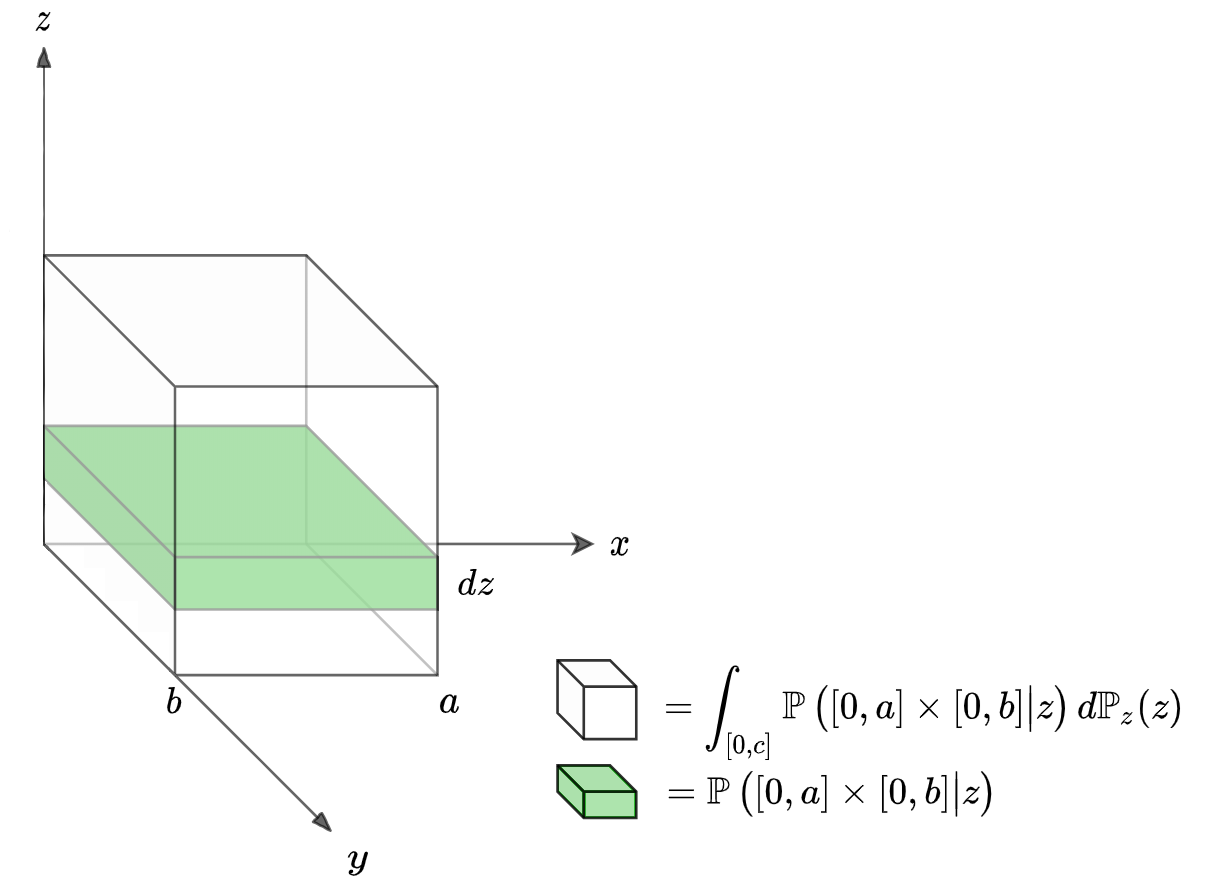
\includegraphics[scale=0.3]{images/disint2.png}
    \caption{ This diagram shows that it is possible to construct a conditional measure to calculate the ``size'' of the green rectangle (whose height tends to 0), however, under the joint measure, such volume evaluates to $0$. The Disintegration Theorem provides us with the construction of such conditional measure.}
    \label{fig:disintegration}
\end{figure}
\subsection{Disintegration Theorem and Conditional Measures}

In this section, we will present the Disintegration Theorem in the context of probability measures, which serves as the extension of the product rule to measures that do not admit the traditional product rule. The product rule is an essential rule in machine learning: for example, it is used in factorising the posterior in Bayesian inference \citep{bayes1763lii}. We will use this theorem to present a derivation for the RN-derivative equivalent of the product rule.

\begin{theorem} (Disintegration Theorem for continuous probability measures): 

For a probability space $(Z, \calB(Z) ,\P)$, where $Z$ is a product space: $Z = Z_x \times Z_y$ and
\begin{itemize}
    \item  $Z_x \subseteq \R^d, Z_y \subseteq \R^{d'}$,
    \item  $\pi_i: Z \rightarrow Z_i$ is a measurable function known as the canonical projection operator (i.e. $\pi_x(z_x,z_y) = z_x$ and $\pi^{-1}_x(z_x) = \{y | \pi_x(z_x) = z\}$),
\end{itemize}
there exists a measure $\P_{y|x}(\cdot | \vx)$, such that
  \begin{align}
      \int_{Z_x \times Z_y} f(\vx, \vy) d\P(\vy) = \int_{Z_x}\int_{Z_y} f(\vx,\vy) d\P_{y|x}(\vy | \vx) d\P(\pi^{-1}(\vx)),
  \end{align}
 where $P_x(\cdot) = \P(\pi^{-1}(\cdot))$ is a probability measure, typically referred to as a pullback measure, and corresponds to the marginal distribution.
\end{theorem}

A direct consequence of the above instance of the disintegration theorem is, with $f(\vx,\vy) = \ind_{A_x \times A_y}(\vx,\vy)$,
\begin{align}
    \P(A_x \times A_y) = \int_{A_x}\P(A_y | \vx) d\P_x(\vx).
\end{align}
 We can see that, in the context of probability measures, the above is effectively analogous to the product rule.

We now have the required ingredients to show the following:

\begin{lemma}\label{lemma:rn_des}(RN-derivative product rule)
Given two probability measures defined on the same product space,  $(Z_x \times Z_y, \calB(Z_x \times Z_y) ,\P)$ and $(Z_x \times Z_y, \calB(Z_x \times Z_y) ,\Q)$, the Radon–Nikodym derivative $\frac{d\P}{d\Q} (\vx,\vy)$ can be decomposed as
\begin{align}
    \frac{d\P}{d\Q} (\vx,\vy) = \frac{d\P_{y|x}}{d\Q_{y|x}}(\vy)\frac{d\P_x}{d\Q_x}(\vx).
\end{align}
\end{lemma}
\begin{proof}

Starting from
\begin{align*}
    \P(A_x \times A_y) =  \int_{A_x}\P(A_y | \vx)  d\P_{x}(\vx),
\end{align*}
we apply the Radon-Nikodym theorem to $\P(A_y | \vx)$ and then to $P_x$:
\begin{align*}
    \P(A_x \times A_y) &=  \int_{A_x}\int_{A_y} \frac{d\P_{y|x}}{d\Q_{y|x}}(\vy) d\Q_{y|x}(\vy) d\P_{x}(\vx) \\
     &= \int_{A_x}\left(\int_{A_y} \frac{d\P_{y|x}}{d\Q_{y|x}}(\vy) d\Q_{y|x}(\vy)\right) \frac{d\P_{x}}{d\Q_{x}}(\vx)d\Q_{x}(\vx) \\
      &= \int_{A_x}\int_{A_y}\frac{d\P_{x}}{d\Q_{x}}(\vx)\frac{d\P_{y|x}}{d\Q_{y|x}}(\vy) d\Q_{y|x}(\vy) d\Q_{x}(\vx).
\end{align*}
Now, via the disintegration we have that
\begin{align*}
  \int_{A_x \times A_y} \frac{d\P_{x}}{d\Q_{x}}(\vx)\frac{d\P_{y|x}}{d\Q_{y|x}}(\vy) d\Q(\vx,\vy) = \int_{A_x}\int_{A_y}\frac{d\P_{x}}{d\Q_{x}}(\vx)\frac{d\P_{y|x}}{d\Q_{y|x}}(\vy) d\Q_{y|x}(\vy) d\Q_{x}(\vx).
\end{align*}
Thus, we conclude that
\begin{align*}
    \P(A_x \times A_y) = \int_{A_x \times A_y} \frac{d\P_{x}}{d\Q_{x}}(\vx)\frac{d\P_{y|x}}{d\Q_{y|x}}(\vy) d\Q(\vx,\vy), 
\end{align*}
which, via the Radon-Nikodym theorem, implies
\begin{align*}
    \frac{d\P}{d\Q} (\vx,\vy) = \frac{d\P_{y|x}}{d\Q_{y|x}}(\vy)\frac{d\P_x}{d\Q_x}(\vx).
\end{align*}
\end{proof}
The above result is used across a variety of different texts in stochastic processes, nonetheless it has proven difficult to find an original source for it and its derivation. We searched through a variety of graduate courses and books on measure and integration and could not find this result, either stated or derived, thus we decided it would be instructive to provide a sketch proof for it, since we will be using it multiple times.


\subsection{RN Derivative of Itô Processes}


As hinted earlier, Itô processes do not admit a PDF, since they are not absolutely continuous with respect to the Lebesgue measure. However, some Itô processes are absolutely continuous with respect to one another, and thus we are able to compute their RN derivatives, useful for calculating the KL divergence between the two processes.  First, we must introduce the following notation:
\begin{definition} (Path measure) \label{def:pathmesu}
    For an Itô process of the form
    \begin{align*}
        d\rvx(t) = \rvb(t) + \rvsigma(t) d\rvw(t),
    \end{align*}
    defined in $[0,T]$, we call $\P$ the path measure of the above process, with outcome space $\Omega=C([0,T], \R^d)$, if the distribution $\P$ describes a weak solution to the above SDE\footnote{Weak solution is a terminology for a solution of an SDE, that does not take into account an initial value problem and has the freedom of specifying its probability space.}.
\end{definition}

In short, the path measure represents the probability measure associated to the stochastic process specified by the SDE.  For example, $\W_{\gamma}$ is the Wiener measure and represents the path measure of a Wiener process with volatility $\sqrt{\gamma}$
 (i.e. $d\rvx(t) = \sqrt{\gamma} d \rvw(t)$). For a more formal introduction to path measures, we require the notion of a \textit{path integral}. We point the reader to \cite{sarkka2019applied, oksendal2003stochastic} for a more thorough introduction.
 
We can now present the following theorem \citep{sarkka2019applied}:
\begin{theorem}\label{thrm:ito_ratio}\citep{sarkka2019applied}
Given two Itô processes with the same constant volatility: 
    \begin{align*}
        d\rvx(t) = \rvb_1(t) + \sigma \rvw(t), \quad \rvx = \rvx_0, \\
        d\rvy(t) = \rvb_2(t) + \sigma\rvw(t), \quad \rvy = \rvx_0,
    \end{align*}
the RN derivative of their respective path measures $\P,\Q$ is given by
\begin{align} \label{eq:girsanov}
    \frac{d\P}{d\Q}(\cdot) = \exp\left(-\frac{1}{2\sigma^2}\int_0^t ||\rvb_1(s) - \rvb_2(s)||^2 ds + \frac{1}{\sigma^2}\int_0^t (\rvb_1(s) - \rvb_2(s))^{\top}d\rvw(s) \right),
\end{align}
\end{theorem}
where the type signature of this RN derivative is $\frac{d\P}{d\Q}: C(T, \R^d) \rightarrow \R$. For example, if  $\rvb_1(s)=\vb_1(\rvx(s), s)$ and $\rvb_2(s)=\vb_2(\rvx(s), s)$ we can write
\begin{align*}
    \frac{d\P}{d\Q}(\vx(t)) = \exp\Bigg(-&\frac{1}{2\sigma^2}\int_0^t ||\vb_1(\vx(s), s) - \vb_2(\vx(s), s)||^2 ds \\ 
    &+ \frac{1}{\sigma^2}\int_0^t \big(\vb_1(\vx(s), s) - \vb_2(\vx(s), s)\big)^{\top}d\rvw(s) \Bigg).
\end{align*}
Note that, in the case where we take the RN derivative with respect to Brownian motion (i.e. $\rvb_2(t) =0, \; \sigma=1$), we have the following expression:
\begin{align} \label{eq:girsanov_0}
    \frac{d\P}{d\W}(\cdot) = \exp\Bigg(-&\frac{1}{2}\int_0^t ||\rvb_1(s) ||^2 ds+ \int_0^t \rvb_1(s)^{\top}d\rvw(s) \Bigg),
\end{align}
which is popularly referred to as Girsanov's theorem, as it is one of the main elements in said theorem.

\section{Summary }

So far, we have introduced a set of self-contained mathematical definitions and results. We have briefly motivated the need for these results and some potentially familiar applications to make them more accessible. Now, we will briefly go over the concepts introduced in this chapter and why we will be needing them:

\begin{itemize}
    \item We have introduced probability measures and defined integration with respect to these measures (i.e.\ the Lebesgue–Stieltjes integral). We require these formalisms in order to write expectations with respect to stochastic processes which do not admit a formulation as a Riemann integral.
    \item We have introduced Brownian motion, path measures and stochastic integrals, which are the core tools needed for representing and manipulating SDEs (Itô processes). SDEs are the main object of study in this thesis and a basic understanding is required to follow some of the algorithms and proofs.
    \item We have provided a sketch proof of a theorem that allows us to decompose the RN derivative (change of measure ratio) of two probability measures analogous to the product rule of probability. We will be using this to decompose and extremise the KL divergence between two SDEs. 
    \item We have presented how to compute the RN derivative between two SDEs, required when computing the KL divergence between SDEs.
\end{itemize}
%\chapter{Background} 
\chapter{The Schrödinger Bridge Problem}

As originally posed by \citet{schrodinger1931uber, schrodinger1932theorie}, the Schrödinger bridge consists of finding a posterior stochastic evolution between two distributions, that is optimally close to a Brownian-motion prior in a KL sense:
\begin{align} \label{eq:schrobirdge}
    \hat{\Q}= \argmin_{\Q \in \calD(\pi_0, \pi_1)} \KL\left(\Q \big|\big| \W\right),
\end{align}
where $\calD(\pi_0, \pi_1)$ represents the set of path measures with marginals $\pi_0$ and $\pi_1$ and:
\begin{align} \label{eq:kl_sho}
    \ \KL\left(\Q \big|\big| \W\right) = \E_{\Q}\left[\ln \frac{d\Q}{d\W}\right].
\end{align}
To the eye of a probabilistic modeller, this objective may be initially quite confusing, mainly because it is minimising the KL divergence between a ``posterior'' distribution $\Q$ and a ``prior'' distribution $\W$, which does not match the usual variational inference objectives that arise from minimising an evidence lower bound \citep{yang2017understanding}. In order to give a sound interpretation to the objective in Equation \ref{eq:schrobirdge}, we will look into the Schrödinger Bridge's formulation as a rare event, and additionally comment on the maximum-entropy-like nature of the objective.

\section{Rare Events and Maximum Entropy }

Let our sample space be the space of random functions with the unit interval as pre-image $C([0,1], \R^d)$, meaning a sample  represents a function of the form $\vx : [0, 1]:  \rightarrow \R^d$.  We now take a set of i.i.d samples $\{\rvx_{i}(t)\}_{i=1}^N$ following standard Brownian motion defined on $C([0,1], \R^d)$. The empirical distribution for $\{\rvx_{i}(t)\}_{i=1}^N$ is defined by
\begin{align}\label{eq:empirical}
    \hat{\W}(A) = \frac{1}{N}\sum_{i=1}^N \ind\left(\rvx_i(t) \in A\right)  , \quad A \in \calB(\R^d)^{[0,1]}.
\end{align}
We, then, might want to find the probability that the empirical distribution prescribes marginals $\pi_0, \pi_1$ which cannot be attained by Brownian motion:
\begin{align}
    {P}\left(\hat{\W} \in \calD(\pi_0, \pi_1) \right).
\end{align}
It turns out that result from the theory of large deviations (Sanov's theorem) allows us to compute an asymptotic expression for such probability \citep{leonard2012schrodinger}:
\begin{align} \label{eq:max_ent}
    {P}\left(\hat{\W} \in \mathcal{D}(\pi_0, \pi_1) \right) \sim \exp\left(-N\inf_{\Q \in \calD(\pi_0, \pi_1)} \!\!\!\!\!\KL\left(\Q \big|\big| \W\right)\right).
\end{align}
For a more technically thorough introduction, please check \cite{leonard2013survey}. Note that the exponent for the probability in Equation \ref{eq:max_ent} extremises the KL divergence, following the principle of minimum discrimination information by \cite{kullback1997information}, which is a generalisation of Edwin Jaynes' maximum entropy principle \citep{jaynes1957information,jaynes2003probability} to continuous distributions. Note, one can observe the connection between maximising entropy and minimising KL divergence by considering the discrete setting, where minimising KL divergence with respect to a uniform reference distribution is equivalent to maximising entropy. In simple words, we are selecting a distribution $\hat{\Q}$, subject to the marginal constraints, that is as close as possible given prior knowledge $\W$.

We can see how the extremisation in the exponent of Equation \ref{eq:max_ent} may be a difficult problem numerically, since it involves two boundary-value constraints, which cannot both be enforced without introducing computational overhead. For example, using the approach of Lagrange multipliers will turn the problem into one of finding a saddle point, rather than a minimisation for which our current tools are better suited.

\section{Dynamic Formulation}
The dynamic formulation of the Schrödinger bridge follows directly from the exponent in the maximum-entropy formulation. The dynamic version of the Schrödinger bridge is written in terms of path measures, that describe the stochastic dynamics defined over the unit interval.
\begin{definition}
    (Dynamic Schrödinger problem) The dynamic Schrödinger problem is given by
    \begin{align}
        \inf_{\Q \in \calD(\pi_0, \pi_1)} \KL\left(\Q \big|\big| \W^{\gamma}\right),
    \end{align}
    where $\Q \in \calD(\pi_0, \pi_1)$ is a path measure with prescribed marginals of $\pi_0, \pi_1$ at times $0, 1$, and $\W_{\gamma}$ is the Wiener measure with volatility $\gamma$ (see Definition \ref{def:pathmesu}). 
\end{definition}
\subsection{As a Stochastic Control Problem}

This formulation of the Schrödinger bridge problem is characterised in terms of extremising a mean-squared-error-styled objective with respect to the drift that describes the SDE for $\Q$. This formulation will allow us to naturally enforce one of the boundary value constraints as an initial value, which will be helpful in the design of an iterative procedure for solving the Schrödinger bridge problem.

The two results presented below are from \cite{pavon1991free}. For pedagogical reasons, we provide a proof sketch of these two results.

We can represent $\Q$ as the distribution which evolves according to the solution of an SDE of the form
\begin{align*}
    d\rvx(t) = \rvb^{+}(t) dt + \sqrt{\gamma} \rvw^+(t).
\end{align*}
\begin{lemma}\citep{pavon1991free}
    The KL divergence between $\Q$ and $\W_{\gamma}$ can be decomposed as
\begin{align}\label{eq:free_energy_1}
     \KL\left(\Q \big|\big| \W^{\gamma}\right) = \KL(p^{\Q}_0 || p_0^{ \W^{\gamma}}) + \E_\Q\left[\int_0^1 \frac{1}{2\gamma}\big|\big|\rvb^{+}(t) \big|\big|^2 dt\right].
\end{align}
We use the notation $p^{\calX}_t$ for the marginal induced by path measure $\calX$, at time $t$. We refer to this expression (Equation \ref{eq:free_energy_1}) as the stochastic control formulation of the Schrödinger bridge problem.
\end{lemma}
\begin{proof}
Via the Disintegration Theorem and Theorem \ref{lemma:rn_des}, we can condition on the endpoint and re-write the RN derivative as
\begin{align*}
    \frac{d\Q}{d\W^{ \gamma}} = \frac{p_0^\Q}{p_0^{ \W^{\gamma}}} \frac{d\Q_{(0,1]}}{d\W_{(0,1]}^{\gamma}}\left(\cdot | \rvx(0) =\vx\right),
\end{align*}
where the disintegration $\Q_{(0,1]}\left(\cdot | \rvx(0) = \vx \right)$ is a solution to $d\rvx(t) = \rvb_t^+ dt + \sqrt{\gamma} \rvw^+(t)$. Then, by Theorem \ref{thrm:ito_ratio}, we can express the RN derivative in terms of  the drift $\rvb_t^+$:
\begin{align*}
    \frac{d\Q}{d\W^{\gamma}} = \frac{p_0^\Q}{p_0^{ \W^{\gamma}}}\exp\left(\int_0^1\frac{1}{2\gamma} \big|\big|\rvb^+(t)\big|\big|^2 dt\right).
\end{align*}
Substituting the above back into the KL divergence completes the result for Theorem \ref{eq:free_energy_1}.
\end{proof}
 We can equivalently express $\Q$ as the solution to a reverse time diffusion:
\begin{align}
    d\rvx(t) = \rvb^{-}(t) dt + \sqrt{\gamma} \rvw^{-}(t), 
\end{align}
where $\rvx(t)$ is adapted to the reverse filtration $(\calF^{-}_i)_{i\in T}$, that is $\calF^{-}_t \subseteq \calF^{-}_s, \; s \leq t$\footnote{This simply means $\rvx(t)$ is only aware about the future.}, and
\begin{align}\label{eq:nelson}
    {\rvb^{+}(t) - \rvb^{-}(t)} =\gamma \nabla_{\vx} p(\rvx(t), t),
\end{align}
where $p(\rvx(t), t)$ is the solution to the FPK equation. The above is typically known as Nelson's duality equation and it relates the forward drift to the dual backward drift \citep{nelson1967dynamical}. 

Using reverse diffusion, \cite{pavon1991free} decompose the KL divergence as done with the forward diffusion:
\begin{lemma}\label{lemma:control}\citep{pavon1991free}
    The KL divergence between $\Q$ and $\W^{\gamma}$ can be decomposed as
\begin{align}\label{eq:free_energy_2}
     \KL\left(\Q \big|\big| \W^{\gamma}\right) = \KL(p^{\Q}_1 || p_1^{ \W^{\gamma}}) + \E_\Q\left[\int_0^1\frac{1}{2\gamma} \big|\big|\rvb^{-}(t)\big|\big|^2 dt\right].
\end{align}
\end{lemma}
Using the drift-based formulations defined above, \cite{pavon1991free} derive alternate (yet equivalent) objectives for the Schrödinger Bridge problem:

\begin{itemize}
\item Forward Objective: 
\begin{align} \label{eq:controlled_bridge_forward}
    \min_{\Q \in \calD(\pi_0, \pi_1)} \KL\big(\Q \big|\big| \W^{\gamma}\big)& = \min_{\rvb^{+} \in \calB }  \E_\Q\left[\int_0^1 \frac{1}{2\gamma}\big|\big|\rvb^{+}(t) \big|\big|^2 dt\right], \nonumber \\
    s.t.\;\;\; d\rvx(t) = \rvb^{+}(t) &dt + \sqrt{\gamma} \rvw^{+}(t), \;\; \rvx(0) \sim \pi_0, \;\; \rvx(1) \sim \pi_1.
\end{align}
\item Backward Objective:
\begin{align} \label{eq:controlled_bridge_backward}
    \min_{\Q \in \calD(\pi_0, \pi_1)} \KL\big(\Q \big|\big| \W^{\gamma}\big)& = \min_{\rvb^{-} \in \calB }  \E_\Q\left[\int_0^1 \frac{1}{2\gamma}\big|\big|\rvb^{-}(t) \big|\big|^2 dt\right], \nonumber \\
    s.t.\;\;\; d\rvx(t) = \rvb^{-}(t) &dt + \sqrt{\gamma} \rvw^{-}(t), \;\; \rvx(1) \sim \pi_1 , \;\; \rvx(0) \sim \pi_0.
\end{align}
\end{itemize}
Where $\calB$ represents the space of admissible control signals or equivalently the space of valid drifts. Notice that the conditioning carried out by the disintegration theorem allows us to remove one of the boundary constraints and integrate it as an initial value problem to the objective. This result inspired us the most in the design of an iterative algorithm for solving the Schrödinger bridge numerically. 
\section{Static Formulation}
\begin{definition}\label{def:static_bridge}
    (Static Schrödinger Problem) The static Schrödinger bridge consists in finding the joint distribution $q(\vx, \vy) \in \calD(\pi_0(\vx), \pi_1(\vy))$, which is closest to the Brownian-motion prior subject to marginal constraints, that is
    \begin{align}\label{eq:static_bridge}
        \inf_{q(\vx,\vy)} \KL (q(\vx,\vy)  &|| p^{\W^{\gamma}}(\vx,\vy)) \nonumber \\
        s.t. \;\;\; \pi_0(\vx) = \int q(\vx,\vy) d\vy, &\;\;\pi_1(\vy) = \int q(\vx,\vy) d\vx.
    \end{align}
\end{definition}
We will now derive this result from the dynamic version. Most surveys and papers on the Schrödinger bridge include some form of this derivation, however they skip several steps which might make it inaccessible. 
\begin{theorem}\citep{follmer1988random}
    The dynamic Schrödinger bridge is solved by
\begin{align}
    \Q^{*} (\cdot) =  \int \W^{\gamma} \left(\cdot | \vx, \vy\right)  q^{*}(\vx,\vy) d\vx d\vy ,
\end{align}
    where $q^*$ is the optimal density that solves the static bridge
    \begin{align*}
        q^{*}(\vx,\vy)& = \arginf_{q(\vx,\vy)} \KL (q(\vx,\vy)  || p^{\W^{\gamma}}(\vx,\vy)),  \\
        s.t. \;\;\; \pi_0(\vx) &= \int q(\vx,\vy) d\vy, \;\;\pi_1(\vy) = \int q(\vx,\vy) d\vx,
    \end{align*}
    and
    \begin{align*}
        \W^{\gamma} \left(\cdot | \vx, \vy\right)  = \W_{(0,1)}^{\gamma}\left(\cdot | \rvx(0) =\vx, \rvx(1) =\vy\right)
    \end{align*}
    is the conditional (disintegration) of the Wiener measure about its endpoints.
\end{theorem} %\vspace{-0.6cm}
\begin{proof}
Firstly, we decompose the KL divergence over path measures $\KL\left(\Q \big|\big| \W\right)$ using Lemma \ref{lemma:rn_des}, and conditioning on the endpoints $\rvx(0), \rvx(1)$ we can re-express the RN derivative as
\begin{align}
    \frac{d\Q}{d\W^\gamma} = \frac{q(\vx, \vy)}{p^{\W^{\gamma}}(\vx, \vy)}\frac{d\Q_{(0,1)}}{d\W_{(0,1)}^\gamma}\left(\cdot | \rvx(0) =\vx, \rvx(1) =\vy\right).
\end{align}
Let $\Q_{(0,1)}(\cdot |  \rvx(0) =\vx, \rvx(1) =\vy) = \Q(\cdot |  \vx,\vy)$. Substituting the above decomposition back into the KL divergence and marginalising where possible, we arrive at 
\begin{align} \label{eq:follmer_kl}
    \KL\left(\Q \big|\big| \W^{\gamma}\right) =&  \KL\left(q(\vx, \vy) \big|\big| p^{\W^{\gamma}}(\vx. \vy) \right)  + \E_{\Q}\left[\frac{d\Q}{d\W^\gamma}\left(\cdot | \vx, \vy\right)\right] \nonumber \\
    =&  \KL\left(q(\vx, \vy) \big|\big| p^{\W^{\gamma}}(\vx. \vy) \right)  + \E_{q(\vx,\vy)}\left[\KL\left(\Q(\cdot |  \vx,\vy)\big|\big|\W^{\gamma}(\cdot |  \vx,\vy)\right)\right].
\end{align}
Notice that the conditional $\Q_{(0,1)}(\cdot |  \rvx(0) =\vx, \rvx(1) =\vy)$ is not affected by the boundary constraints, thus we can set $\Q(\cdot | \vx,\vy) = \W^\gamma\left(\cdot | \vx, \vy\right)$, making the second term 0, and leaving us with the static bridge. It then suffices to reverse the disintegration theorem, in order to build up $\Q^{*}$ from $q^{*}$ and $\Q^{*}(\cdot | \vx,\vy)$, completing the proof.
\end{proof}

The earliest references we found for the above result are given by \cite{follmer1988random}, where the decomposition of the KL divergence for two diffusions (Equation \ref{eq:follmer_kl}) is provided. However, we were not able to find a good reference for Lemma \ref{lemma:rn_des} and thus we have provided an instructive derivation for it.
\subsection{As an Entropy-Regularised Optimal Transport Problem}

The optimal transport problem in its intuitive form is concerned with the transportation of a distribution into another distribution, subject to cost $c(\vx,\vy)$. In its discrete histogram-based formulation, it is referred to as the earth mover's distance (EMD) \citep{levina2001earth}, since it can be illustrated as moving dirt between two piles of earth. One of the early applications of EMD was in comparing grey-scale images for the development of an image retrieval system. 

\begin{definition}
Formally, the optimal transport problem is given by the following objective:
\begin{align*}
\inf_{Q \in \calD(\pi_0, \pi_1)}\int  c(\vx, \vy) dQ(\vx, \vy),
\end{align*}
and if $Q$ is absolutely continuous w.r.t.\ to the Lebesgue measure, we can express the above as
\begin{align*}
\inf_{Q \in \calD(\pi_0, \pi_1)}\int \int c(\vx, \vy) q(\vx, \vy) d\vx d\vy.
\end{align*}
Furthermore, when $ c(\vx, \vy) = || \vx - \vy||^2$, the above resembles the square of the Wasserstein distance $\calW^2_{2}(\pi_0, \pi_1)$.
\end{definition}

Here, we will present and discuss a very well-studied \citep{mikami2008optimal,leonard2012schrodinger,leonard2013survey,carlier2017convergence} connection between the static bridge and the Wasserstein distance.  For the Wiener process $\W^\gamma$ prior, we have
\begin{align}
    p^{\W^{\gamma}}(\vx,\vy) = p^{\W^{\gamma}}_0(\vx)\calN(\vy | \vx, \gamma\I),
\end{align}
and the term
\begin{align*}
    \int q(\vx, \vy)\ln  p^{\W^{\gamma}}_0(\vx) d\vx d\vy =  \int \pi_0(\vx) \ln  p^{\W^{\gamma}}_0(\vx) d\vx 
\end{align*}
does not depend on $q$ (due to the constraints). Substituting the above into Equation \ref{eq:static_bridge}, we arrive at
\begin{align}
    &\inf _{q \in \calD(\pi_0, \pi_1)}\int \int -\frac{||\vx - \vy ||^2}{2\gamma} q(\vx, \vy) d\vx d\vy  + \int \int q(\vx, \vy) \ln q(\vx, \vy) d\vx d\vy, \nonumber \\
    &=\inf _{q \in \calD(\pi_0, \pi_1)}\int \int -\frac{||\vx - \vy ||^2}{2} q(\vx, \vy) d\vx d\vy  - \gamma \text{H} \left(q(\vx, \vy)\right),
\end{align}
which is an entropy-regularised optimal mass transport problem (OMT) \citep{villani2003topics} with a quadratic cost function. Furthermore, as the volatility/noise of the Brownian-motion prior goes to 0 ($\gamma \downarrow 0$), the above quantity converges to $\calW^2_{2}(\pi_0, \pi_1)$ (squared Wasserstein distance in an $L_2$ metric space).
\subsection{The Schrödinger System}

Following \cite{pavon2018data}, the Lagrangian of Equation \ref{eq:static_bridge} is given by
\begin{align}\label{eq:schro_lagrangian}
    \calL(q, \lambda,  \mu) &=  \KL (q(\vx,\vy)  || p^{\W^{\gamma}}(\vx,\vy))  \nonumber\\
    &+ \int \lambda(\vx)\left( \int q(\vx,\vy)d\vy -\pi_0(\vx)\right)d\vx \nonumber \\
    &+ \int \mu(\vy) \left(\int q(\vx,\vy) d\vx - \pi_1(\vy)\right) d\vy.
\end{align}
Let $p^{\W^{\gamma}}(\vx,\vy) = p^{\W^{\gamma}}_0(\vx)p^{\W^{\gamma}}(\vy|\vx)$, where $p^{\W^{\gamma}}_0(\vx)$ is the marginal prior, which we are free to set, and $p^{\W^{\gamma}}(\vy|\vx)=\calN(\vy | \vx, \gamma\I)$ is the transition density of the prior. Then, we set the functional derivative $\frac{\delta \calL}{\delta q(\vx, \vy)}$ to 0 and obtain
\begin{align*}
    1 + \ln q(\vx, \vy)  - \ln p^{\W^{\gamma}}(\vy|\vx)
    - \ln p^{\W^{\gamma}}_0(\vx)+ \lambda(\vx)
+ \mu(\vy) = 0. \nonumber
\end{align*}
Rearranging, we get
\begin{align*}
{q^{*}(\vx, \vy) }  = \exp\left(  \ln p^{\W^{\gamma}}_0(\vx) -\lambda(\vx) -1\right)p^{\W^{\gamma}}(\vy|\vx)\exp\left(- \mu(\vy)\right) ,\nonumber
\end{align*}
which we can re-express in terms of the auxiliary potentials $\hphi_0(\vx), \phi_1(\vy)$:
\begin{align*}
{q^{*}(\vx, \vy) }  = \hphi_0(\vx)p^{\W^{\gamma}}(\vy|\vx)\phi_1(\vy), \nonumber
\end{align*}
satisfying
\begin{align}
    \hphi_0(\vx) \int \phi_1(\vy) p^{\W^{\gamma}}(\vy|\vx) d\vy = \pi_0(\vx) , \nonumber\\ 
    \phi_1(\vy) \int \hphi_0(\vx) p^{\W^{\gamma}}(\vy|\vx) d\vx = \pi_1(\vy), \nonumber
\end{align}
where we re-label the terms with the integrals to
\begin{align} \label{eq:sysint}
    \phi_0(\vx) &= \int \phi_1(\vy) p^{\W^{\gamma}}(\vy|\vx) d\vy, \nonumber\\ 
    \hphi_1(\vy) &= \int \hphi_0(\vx) p^{\W^{\gamma}}(\vy|\vx) d\vx. \nonumber
\end{align}
Putting it all together, the following linear functional system is known as the Schrödinger system:
\begin{align}
    \hphi_0(\vx) \phi_1(\vx)  = \pi_0(\vx),  \nonumber \\ 
    \hphi_1(\vx) \phi_1(\vy)  = \pi_1(\vy).
\end{align}
We obtain the distribution $\pi^{*}_t(\vz)$ (solution to the FPK equation for the optimal $Q^{*}$):
\begin{align}
    \pi^{*}_t(\vz) =  \hphi_t(\vz) \phi_t(\vz) ,
\end{align}
where
\begin{align}
    \phi_t(\vz) &= \int \phi_1(\vy(1) ) p^{\W^{\gamma}}(\vy(1)|\vz(t)) d\vy(1), \nonumber\\ 
    \hphi_t(\vz) &= \int \hphi_0(\vx(0)) p^{\W^{\gamma}}(\vz(t)|\vx(0)) d\vx(0). \nonumber
\end{align}
Note that, by Proposition 3.3 of \cite{pavon1991free}, the optimal control signal/drift $\rvb_t^+$ can be recovered from the solution of the Schrödinger system:
\begin{align} \label{eq:drifr_potential}
    \rvb_t^{+} = \gamma \nabla \ln \phi_t(\vx(t) ).
\end{align}

The Schrödinger system is an equivalent formulation to the static Schrödinger problem in terms of the potential functions. It is by no means a method or an algorithm for solving the problem. One can solve the system in closed form, when the integrals in Equation \ref{eq:sysint} admit a simple solution, by guessing for the potentials in a similar way to how we formulate an \textit{ansatz} for simple differential equations. 

\section{Half Bridges}

Having only one boundary constraint simplifies the original problem, since it becomes trivial to enforce such constraint numerically. In this section, we will study in more detail such single-constraint problems and illustrate why exactly it is a simpler problem. This construction will be of use, since it will constitute part of the steps in the final algorithms for solving the full bridge problem.

The half-bridge problem, as presented in \cite{pavon2018data}, is a simpler variant of the full Schrödinger bridge with only one boundary constraint. 

\begin{definition}
The forward half bridge is given by
    \begin{align}
        {\Q}^{*} = \inf_{\Q  \in \calD(\pi_0, \cdot)} \KL (\Q || \W^\gamma) .
    \end{align}
\end{definition}
\begin{theorem}\label{thrm:half_bridge_forward}
    The forward half bridge admits the following solution: 
\begin{align}
    {\Q}^{*}\left(A_0 \times A_{(0,1]}\right) =  \int_{A_0\times A_{(0,1]}} \frac{d \pi_0}{ dp_0^{\W^\gamma}} d\W^\gamma.
\end{align}
\end{theorem}
\begin{proof}
Via the disintegration theorem, we have the following decomposition of KL:
\begin{align}
    \KL(\Q || \W^\gamma) = \KL(p_0^\Q|| p_0^{\W} )  + \E_p\left[\KL(\Q(\cdot| \vx) || \W^\gamma(\cdot | \vx))\right]. \nonumber
\end{align}
Thus, via matching terms accordingly, we can construct $\Q^*$ by setting $\Q(\cdot| \vx)=\W^{\gamma}(\cdot| \vx)$ and matching the constraints:
\begin{align}
    {\Q}^{*}\left(A_0 \times A_{(0,1]}\right) = \int_{A_0 \times A_{(0,1]}}\!\!\!\!\!\!\!\!\!\!\!\!\W^\gamma(A_{(0,1]} | \vx) d\pi_0(\vx),
\end{align}
\begin{align}
    {\Q}^{*} &= \int_{A_0}  \frac{d\pi_0}{dp_0^{\W^\gamma}}(\vx)   \W^\gamma(\cdot | \vx) d p_0^{\W^{\gamma}}(\vx) \nonumber \\
    &= \int_{A_0 \times A_{(0,1]} }  \frac{d\pi_0}{dp_0^\W}(\vx)  d \W^{\gamma}.
\end{align}
\end{proof}
\begin{definition}
The backward half bridge is given by
    \begin{align}
        {\P}^{*} = \inf_{\P  \in \calD(\cdot, \pi_1)} \KL (\P || \W^\gamma) .
    \end{align}
\end{definition}
\begin{theorem}\label{thrm:half_bridge_backward}
     The backward half bridge admits the following solution: 
\begin{align}
    {\P}^{*}\left( A_{[0,1)} \times A_1\right) =  \int_{ A_{[0,1)} \times A_1}  \frac{d \pi_1}{ d p_1^{\W^\gamma} } d\W^\gamma.
\end{align}

\end{theorem}
\begin{proof}
Same as Theorem \ref{thrm:half_bridge_forward}.
\end{proof}


Note how the main difference between the full and half bridges is that the half bridges admit a closed-form solution in terms of known quantities. Similarly to the full bridge, the half bridges admit a static formulation:

\begin{definition}
The static forward bridge is given by the following objective:
 \begin{align}\label{eq:static_bridge_forward}
        \inf_{q(\vx,\vy)} \KL  &(q(\vx,\vy) || p^{\W^{\gamma}}(\vx,\vy)), \nonumber \\
        s.t. \;\;\;& \pi_0(\vx) = \int q(\vx,\vy) d\vy.
\end{align}
\end{definition}
\begin{theorem}\label{thrm:static_half_forward}
     The static forward bridge admits the following solution:
     \begin{align}
         q^{*}(\vx,\vy) = p^{\W_{\gamma}}(\vx, \vy)\frac{\pi_0(\vx)}{p^{\W_{\gamma}}(\vx)}.
     \end{align}
\end{theorem}
\begin{proof}
See \cite{pavon2018data} for the solution of the backward half bridge. Proof is simple and easy to adapt to the forward bridge. 
\end{proof}
\begin{definition}
The static backward bridge is given by the following objective:
 \begin{align}\label{eq:static_bridge_backward}
        \inf_{p(\vx,\vy)} \KL  &(p(\vx,\vy) || p^{\W^{\gamma}}(\vx,\vy)), \nonumber \\
        s.t. \;\;\;& \pi_1(\vy) = \int p(\vx,\vy) d\vx. 
\end{align}
\end{definition}
\begin{theorem}\label{thrm:static_half_backward}
     The static backward bridge admits the following solution:
     \begin{align}
         p^{*}(\vx,\vy) = p^{\W_{\gamma}}(\vx, \vy)\frac{\pi_1(\vy)}{p^{\W_{\gamma}}(\vy)}.
     \end{align}
\end{theorem}
\begin{proof}
See \cite{pavon2018data}.
\end{proof}

Half bridges are a significantly easier problem than full bridges. Not only do they admit ``closed-form'' solutions in some sense, they also allow removing constraints by incorporating them as an initial value problem. Going forward, we will see how to build an iterative scheme for solving the full bridge that makes use of solving half bridge sub-problems at each iteration.

\section{Summary}
 In this chapter, we have introduced the dynamic and static formulations of the Schrödinger bridge problem, together with the following equivalent formulations:
 \begin{itemize}
     \item A stochastic control formulation that parametrises the dynamic bridge in terms of a drift and allows to incorporate a boundary constraints as an initial value problem.
     \item A system of functions known as the Schrödinger system, parametrised in terms of potentials. The solution of this system solves the static Schrödinger bridge. 
 \end{itemize}
 We will be using these alternate formulations in the design of numerical algorithms for solving the Schrödinger bridge problem.
%\chapter{Algorithmic Framework} 
\chapter{Iterative Proportional Fitting Procedure}

So far we have introduced the Schrödinger bridge problem as well as its simpler half bridge variant. We have also introduced the Schrödinger system and loosely hinted at a potential iterative solution, but we have not yet presented a full solution and discussed its guarantees/properties.

In this chapter, we will study an algorithmic framework known as the Iterative Proportional Fitting Procedure (IPFP) \citep{csiszar1975divergence, kullback1968probability, ruschendorf1995convergence,cramer2000probability} and describe its usage for solving the Schrödinger bridge. Furthermore, we will formalise a previously made observation that connects Fortet's Iterative scheme \citep{fortet1940resolution} for solving the Schrödinger system with the more general IPFP. 

\section{Fortet's Algorithm}

Let us start by introducing Fortet's algorithm, which is maybe the oldest algorithm with a proof of convergence \citep{fortet1940resolution} for solving the Schrödinger system.

\begin{algorithm} \label{alg:fortet}
\SetKwInOut{Input}{input}
\Input{$\pi_0(\vx), \pi_1(\vy), p(\vy | \vx)$}
Initialise $\phi_0^{(0)}(\vx)$ such that $\phi_0^{(0)}(\vx) <\!< \pi_0(\vx)$ \\
    \Repeat{convergence}{
      $\hphi_0^{(i)}(\vx) := \frac{\pi_0(\vx)}{\phi_0^{(i)}(\vx)}$ \\
      $\hphi_1^{(i)}(\vy) := \int  p(\vy | \vx) \hphi_0^{(i)}(\vx) d\vx$ \\
      $\phi_1^{(i)}(\vy) := \frac{\pi_1(\vy)}{\hphi_1^{(i)}(\vy)}$ \\
      $\phi^{(i+1)}_0(\vx) := \int  p(\vy | \vx) \phi_1^{(i)}(\vy) d\vy$\\
      $i:=i+1$
    }
\Return{$\hphi_0^{(i)}(\vx), \phi_1^{(i)}(\vy)$}
\caption{Fortet's Iterative Procedure}
\end{algorithm}
Modern adaptations for the proof of convergence for Algorithm  \ref{alg:fortet} can be found in \citep{essid2019traversing, chen2016entropic}, however, these proofs are beyond the scope of this thesis. Let us now provide an intuition behind each step in the algorithm:

\begin{itemize}
    \item $\hphi_0^{(i)}(\vx) := \frac{\pi_0(\vx)}{\phi_0^{(i)}(\vx)}$: enforces the marginal/boundary constraint at time $0$. That is, it enforces that the product of the factors/potentials matches the marginal distribution $\pi_0$.
    \item $\hphi_1^{(i)}(\vy) := \int  p(\vy | \vx) \hphi_0^{(i)}(\vx) d\vx$ : Now that we have the factors $\phi_0^{(i)}(\vx) \hphi_0^{(i)}(\vx) $ $:= {\pi_0(\vx)}$ for the marginal at $t=0$, we transport/transition them to the marginal at time $t=1$ by marginalising the current estimate of the joint posterior $\pi_1(\vy) = \phi_1(\vy) \int p(\vy| \vx) \hphi_0^{(i)}(\vx) d\vx$.
    \item  $\phi_1^{(i)}(\vy) := \frac{\pi_1(\vy)}{\hphi_1^{(i)}(\vy)}$: As with $t=0$, we enforce the marginal/boundary  constraint such that  $\phi_1^{(i)}(\vy) \hphi_1^{(i)}(\vy) := {\pi_1(\vy)}$. 
    \item $\phi^{(i+1)}_0(\vx) := \int  p(\vy | \vx) \phi_1^{(i)}(\vy) d\vy$: Now that we have enforced the constraint for $t=1$, we marginalise our current estimate of the joint to move from $\vy$ to $\vx$ and repeat.
\end{itemize}

 The potential at time $t=0$ is initialised with the prior marginal. Then, we iterate the Schrödinger system until reaching a fixed point.  The marginal constraints are satisfied by alternating between the $t=0$ and $t=1$ marginals. This leads us to the following observation:
\begin{observation}\label{obs:forkek}
Fortet's algorithm starting at $t=1$, rather than $t=0$, is equivalent to sequentially alternating between solving forward and backward static half bridges.
\begin{algorithm} \label{alg:ipfp_intro}
\SetKwInOut{Input}{input}
\Input{$\pi_0(\vx), \pi_1(\vy), p(\vy | \vx)$}
Initialise:\\
$p^{\W^{\gamma}}_1(\vy)$ such that $p^{\W^{\gamma}}_1(\vy) <\!< \pi_1(\vy)$ \\
$ q^{*}_{0}(\vx,\vy) :=p^{\W^{\gamma}}(\vx,\vy)$\\
$i=0$ \\
    \Repeat{convergence}{
      $i := i + 1$ \\
     $ p^{*}_{i}(\vx,\vy) = \inf_{p(\vx,\vy) \in \calD( \cdot, \pi_1)} \KL  (p(\vx,\vy) || p^{*}_{i-1}(\vx,\vy))$\\ 
     $ q^{*}_{i}(\vx,\vy)  = \inf_{q(\vx,\vy) \in \calD(\pi_0, \cdot)} \KL  (q(\vx,\vy) ||  p^{*}_{i}(\vx,\vy))$
    }
\Return{$q^{*}_{i}(\vx,\vy) , p{*}_{i}(\vx,\vy)$}
\caption{Alternating half bridges (\cite{kullback1968probability} IPFP) }
\end{algorithm}
\end{observation}
\begin{proof}
Consider the first two iterations of Algorithm \ref{alg:ipfp_intro}:

Using Theorem \ref{thrm:static_half_backward}, the solution to the backward half bridge
 \begin{align}
        \inf_{p(\vx,\vy) \in \calD( \cdot, \pi_1)} \KL  &(p(\vx,\vy) || p^{\W^{\gamma}}(\vx,\vy)) \nonumber 
\end{align}
is
\begin{align}
    p_0^{*} (\vx, \vy) = p^{\W^{\gamma}}_0(\vx) p^{\W^{\gamma}}(\vy| \vx) \frac{\pi_1(\vy)}{p^{\W^{\gamma}}_1(\vy)}.
\end{align}
We set up the following forward bridge:
\begin{align}
    \arginf_{q_0(\vx, \vy)  \in \calD(\pi_0 , \cdot)}\KL (q_0(\vx, \vy) ||p_0^{*} (\vx, \vy)),
\end{align}
which, following Theorem \ref{eq:static_bridge_forward}, can be solved by
\begingroup
\allowdisplaybreaks
\begin{align}
    q_0^{*} (\vx, \vy) &= p_0^{*} (\vx, \vy) \frac{\pi_0(\vx)}{p_0^{*} (\vx)} \\
 &=  p^{\W^{\gamma}}(\vy| \vx) \frac{\pi_1(\vy)}{p^{\W^{\gamma}}_1(\vy)} \frac{\pi_0(\vx)}{\int   p^{\W^{\gamma}}(\vy| \vx) \frac{\pi_1(\vy)}{p^{\W^{\gamma}}_1(\vy)} d\vy}.
\end{align}
\endgroup

If we proceed to the second iteration of this procedure, the backward bridge step will yield
\begin{align}
    p_1^{*} (\vx, \vy) =  q_0^{*} (\vx, \vy) \frac{p^{\W^{\gamma}}_1(\vy)}{ \underbrace{\displaystyle\int \frac{p^{\W^{\gamma}}(\vy| \vx)\pi_0(\vx)}{\int p^{\W^{\gamma}}(\vy| \vx) \frac{\pi_1(\vy)}{p^{\W^{\gamma}}_1(\vy)} d\vy}d\vx}_{{\phi}^{1}(\vy)}} ,
\end{align}
and the forward step:
\begin{align}
    q_1{*} (\vx, \vy) &= p_1^{*} (\vx, \vy) \frac{\int    p^{\W^{\gamma}}(\vy| \vx) \frac{\pi_1(\vy)}{p^{\W^{\gamma}}_1(\vy)}  d \vy}{\int    p^{\W^{\gamma}}(\vy| \vx) \frac{\pi_1(\vy)}{{\phi}^{1}(\vy)}  d \vy}.
\end{align}
Re-labeling, we get 
\begin{align}
    \phi^0(\vy)&=p^{\W^{\gamma}}_1(\vy), \\ 
    \hat{\phi}_0^{i}(\vx) &= \int  p^{\W^{\gamma}}(\vy| \vx) \frac{\pi_1(\vy)}{{\phi}^{i}(\vy)}  d \vy,
\end{align}
and we can make an inductive argument on $i$ for the following inductive hypothesis\footnote{Some simple term-cancellation steps have been omitted to reduce verbosity.}:
\begin{align} \label{eq:recurrence}
  {\phi}^{i+1}(\vy) =  \displaystyle\int \frac{p^{\W^{\gamma}}(\vy| \vx)\pi_0(\vx)}{\int p^{\W^{\gamma}}(\vy| \vx) \frac{\pi_1(\vy)}{\phi^i(\vy)} d\vy}d\vx,
 \end{align}
 \begin{align}
  p_i^{*} (\vx, \vy) =   q_{i-1}^{*} (\vx, \vy) \frac{\phi^{i-1}(\vy)}{{\phi}^{i}(\vy)} ,
\end{align}
 \begin{align}
      q_i{*} (\vx, \vy) =     p_i^{*} (\vx, \vy) \frac{\hat{\phi}_0^{i-1}(\vx)}{\hat{\phi}_0^{i}(\vx)} .
\end{align}
We can see that the  recurrence in Equation \ref{eq:recurrence} is the exact same set of steps performed by Fortet's algorithm, if we were to reverse the time order or start Fortet's algorithm at step 5 and consider the first steps  as an initialisation of $\phi_0(\vy)$.
\end{proof}

Whilst in hindsight the above observation may seem simple, we regard it as a contribution, as we have not observed a formal argument made towards this connection. As we will see in the following sections, Observation \ref{obs:forkek} establishes a link between Fortet's algorithm and algorithms derived from the iterative proportional fitting procedure.

\section{Kullback's IPFP}
The original iterative proportional fitting procedure (IPFP) consists of estimating a normalised contingency table (discrete joint distribution) given prescribed marginals, via some form of information-discrimination/maximum-entropy principle. However, we are interested in the continuous variant of IPFP, which dates back to Kullback \citep{kullback1968probability}.

What we call in this section Kullback's IPFP is in fact Algorithm \ref{alg:ipfp_intro}, which we have introduced via its formal connection to Fortet's algorithm.  The first complete proof of convergence to Algorithm \ref{alg:ipfp_intro} was provided in \cite{ruschendorf1995convergence}, using information-geometric arguments from \cite{csiszar1975divergence}.

\section{Generalised IPFP}

\begin{figure}[t!]
    \centering
    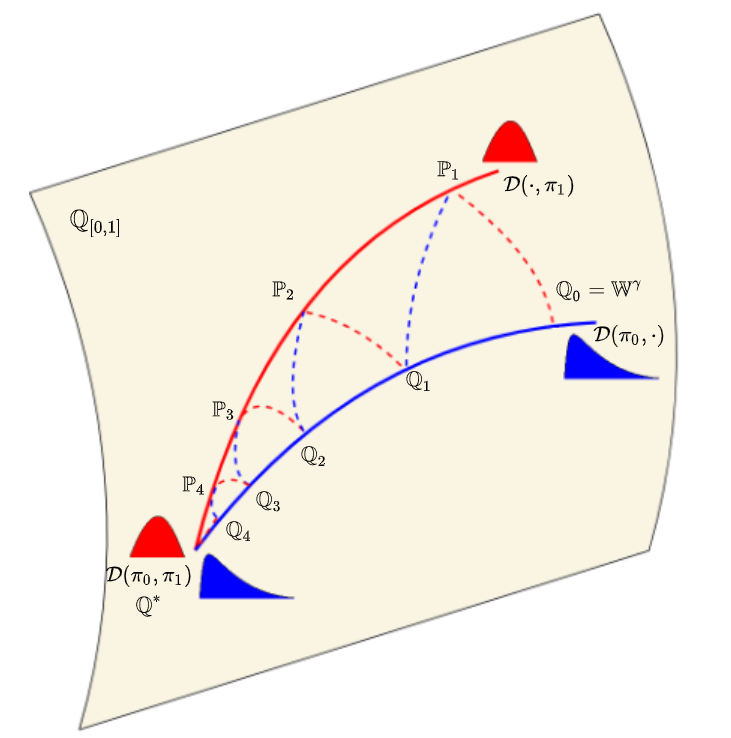
\includegraphics[]{images/g-IPFP_ready.PNG}
    \caption{Illustration of the iterative proportional fitting procedure, inspired and adapted from Figure 1 in \cite{bernton2019schr}. The red line represents valid Itô-process posteriors with the terminal constraint $\P \in \calD(\cdot, \pi_1)$, and the blue represents valid Itô-process posteriors with the initial constraint $\Q \in \calD( \pi_0, \cdot)$. The illustration shows the alternation between the forward and backward steps, until the joint-bridge solution is reached where both constraints are met. Note the sheet represents the space of all valid Itô processes in the interval $[0,1]$. By valid we mean Itô processes driven by the prior of the form $d\rvx(t) = \rvb_t + \gamma d\rvw(t)$.}
    \label{fig:info_pro}
\end{figure}

We call generalised iterative proportional fitting procedure (g-IPFP) the extension of the continuous IPFP, initially proposed by Kullback to a more general setting over path measures, as presented in \cite{cramer2000probability, bernton2019schr}. The method is identical to the regular IPFP, only that it re-states the problem in terms of probability measures.
\begin{algorithm} \label{alg:gipfp}
\SetKwInOut{Input}{input}
\Input{$\pi_0(\vx), \pi_1(\vy), \W^{\gamma}$}
Initialise:\\
$\Q^{*}_0 =\W^{\gamma}$\\
$i=0$ \\
    \Repeat{convergence}{
      $i := i + 1$ \\
     $ \P_i^{*} = \inf_{\P \in \calD( \cdot, \pi_1)} \KL  (\P|| \Q^{*}_{i-1})$\\ 
     $ \Q_i^{*}  = \inf_{\Q \in \calD(\pi_0, \cdot)} \KL  (\Q||  \P^{*}_{i})$
    }
\Return{$\Q_i^{*}, \P_i^{*}$}
\caption{g-IPFP \citep{cramer2000probability} }
\end{algorithm}

Using Theorems \ref{thrm:half_bridge_forward} and \ref{thrm:half_bridge_backward}, steps 6 and 7 of Algorithm \ref{alg:gipfp} can be expressed in ``closed form'' in terms of known quantities:
\begin{align}
    {\P}^{*}_i\left( A_{[0,1)} \times A_1\right) =  \int_{ A_{[0,1)} \times A_1}  \frac{d \pi_1}{ d p_1^{\Q^{*}_{i-1}}} d\Q^{*}_{i-1},
\end{align}
\begin{align}
    {\Q}^{*}_i\left(A_0 \times A_{(0,1]}\right) =  \int_{A_0\times A_{(0,1]}} \frac{d \pi_0}{ dp_0^{\P^{*}_i}} d\P^{*}_i.
\end{align}
An important thing to note about the above solutions is that while these quantities are written in terms of components that we ``know'', such components are themselves not available in closed form and require some form of approximation scheme (e.g.\ Monte Carlo integration) in order to be computed.

Via the disintegration theorem, we can reduce g-IPFP to the standard IPFP, by noting that $\Q^*_i(\cdot |\vx,\vy) =\P^*_i(\cdot |\vx,\vy) = \W(\cdot |\vx,\vy)$ remains invariant across iterations, thus we highlight that more than being an algorithm, g-IPFP serves as a framework for the development and design of algorithms aimed at solving the Schrödinger Bridge.

The proof from \cite{ruschendorf1995convergence} extends naturally to g-IPFP, as mentioned in \cite{bernton2019schr}. Furthermore, \cite{bernton2019schr} provide additional results regarding the convergence rate of g-IPFP.
\begin{figure}[h!]
    \centering
    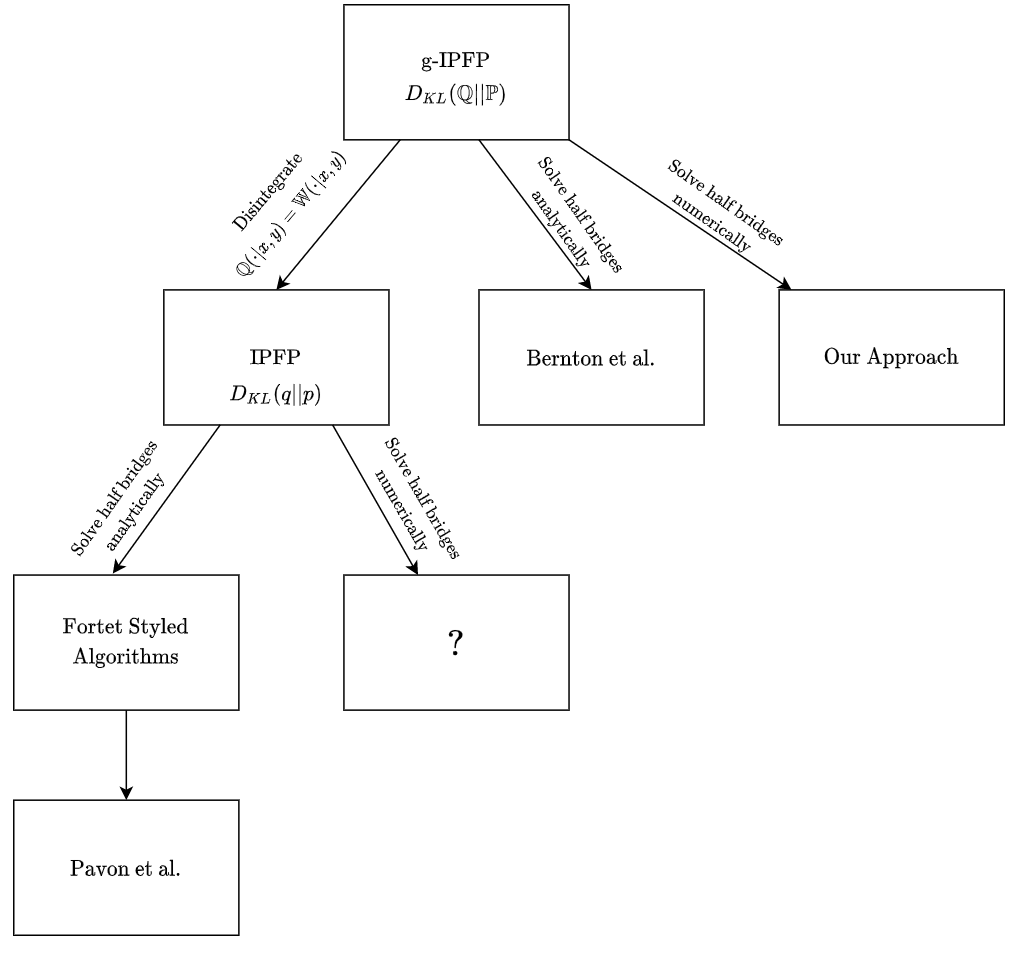
\includegraphics[width=\linewidth]{images/IPFP_Geanology.png}
    \caption{Genealogy of IPFP-based algorithms for solving the Schrödinger bridge problem. ``?'' symbolises an area without much prior research.}
    \label{fig:genealogy}
\end{figure}

%\chapter{Related Work} 
\chapter{Related Problems}
We have presented the Schrödinger bridge, as well as an algorithmic framework for solving it. In this chapter, we will compare the Schrödinger bridge and IPFP to two different methodologies employed in machine learning for mapping between distributions. 
\section{Continuous-Time Stochastic Flows}

Imagine that, as a probabilistic modeller, you were given the problem of mapping from one distribution to another. One of the simplest ways of approaching such task is to specify a generative process of the form
\begin{align*}
    \rvx &\sim \pi_0, \\
    \rvy &= \calT_{\theta}(\rvx),
\end{align*}
where $\calT_{\theta}(\rvx)$  is a stochastic mapping (i.e.\ $\calT_{\theta}(\rvx) = f_{\theta}(\rvx) + \rvepsilon$). Then, to learn the mapping $\calT_{\theta}(\rvx)$, we maximise the marginal likelihood for a set of observations $\{\vy_i \sim \pi_1 \}$:
\begin{align*}
   \argmax_{\theta} \prod_i p(\vy_i) = \argmax_{\theta} \prod_i \int p_{\theta}(\vy_i | \vx) d\pi_0(\vx).
\end{align*}

We can take a further step and model the relationship between the two distributions using an SDE:
\begin{align*}
    \rvx(0) &\sim \pi_0, \\
    d\rvx(t) &= \vb_{\theta}(\rvx(t), t) + \sqrt{\gamma} d\rvw(t), \\
    \rvy &= f_{\theta}(\rvx(1)).
\end{align*}
In other words: $\rvy$ is generated by the solutions to an SDE with initial distribution $\pi_0$. We can also interpret the above as the latent object living in path space (i.e. $C([0,1],\R^d)$), as we have no observations for the trajectories, but only observations of its initial and terminal distributions. Similarly to the latent-variable-model example, we aim to maximise an estimate of the marginal likelihood under this generative process. Variants of this approach are explored by \citep{lahdesmakideep, tzen2019neural} as ways of having infinitely-deep neural networks and Gaussian processes.

It is clear that this approach is different to the Schrödinger bridge. Firstly, the generative process requires the observation of pairs $\vx_i, \vy_i$ in order to estimate the marginal likelihood. Secondly, the Schrödinger bridge is based on the principle of maximum entropy \citep{jaynes1957information}, whilst this generative approach is based on maximising a marginal likelihood (ML-II). However, they share the similarity of exploiting stochastic dynamics to relate source and target distributions. Additionally, both have similar notions of prior and posterior dynamics.

\section{Domain Adaptation and Generative Adversarial Networks (GANs)}

In this section, we will motivate and provide some formal arguments towards the following observation:
\begin{observation}
Each half-bridge objective in the IPFP algorithm is equivalent to a GAN-like objective with a corresponding cycle-consistency term, up to a regularisation term.
\end{observation}

\subsection{Short Introduction to Domain Adaptation with GANs}

The goal of a GAN \citep{goodfellow2014generative} is to fit a generative model of the form
\begin{align*}
    \rvx &\sim \pi_0, \\
    \rvy &= f_{\theta}(\rvx),
\end{align*}
in the setting where we can sample from $\pi_0(\vx)$ and $\pi_1(\vy)$ tractably. The above model induces likelihood $p_{\theta}(\vy | \vx)$ and marginal $p_{\theta}(\vy)$, however the marginal is never computed explicitly and, thus, sometimes fitting GANs is referred to as fitting implicit generative models \citep{mohamed2016learning}.

Using our notation, the GAN-fitting procedure \citep{goodfellow2014generative} takes the following form:

\begin{itemize}
    \item (Discriminator loss) Estimating the surrogate to later be fitted by model $p_{\theta}(\vy)$:
 $$ {\beta}^{*} = \argmin_{\beta} \left(\alpha \E_{\pi_1(\vy)}[-\log D_{\beta}(\vy)] + (1-\alpha)\E_{p_{\theta}(\vy)}[-\log (1-D_{\beta}(\vy))]\right).$$ 
 \item (Generative loss) Fitting model $p_{\theta}(\vy)$ on the estimated surrogate:
 $$\theta^{*} = \argmin_{\theta}-\E_{p_{\theta}(\vy)}\left[\log(D_{\hat{\beta^{*}}}(\vy))\right].$$ 
\end{itemize}

In practice, the generator step \citep{goodfellow2014generative} typically minimises $-\E_{p_{\theta}(\vy)}\left[\log(D(\vy))\right]$, which according to \cite{goodfellow2014generative} is equivalent to maximising  $\E_{p_{\theta}(\vy)}\left[\log(1-D(\vy))\right]$.

The task of domain adaptation in GANs is finding a mapping between two distributions $\pi_0, \pi_1$ that have been observed empirically. This has applications in image and language translation \citep{zhu2017unpaired,lample2017unsupervised}. Typically, in domain adaptation with GANs, the following two processes are fitted in parallel:
\begin{align*}
    \rvx &\sim \pi_0,    &\rvy &\sim \pi_1,\\
    \rvy &= f_{\theta}(\rvx),   &\rvx &= g_{\phi}(\rvy).
\end{align*}
An interesting variation of GANs, used for domain adaptation and known as Cycle-GAN, adds an extra term to the generative loss, called the cycle-consistency loss:
\begin{align*}
   \E_{\vx \sim \pi_0}\left[ \Big|\Big|\vx- g_\phi\left(f_\theta(\vx) \right) \Big|\Big|^2\right] +  \E_{\vy \sim \pi_1}\left[ \Big|\Big|\vy- f_\theta\left(g_\phi(\vy) \right) \Big|\Big|^2\right].
\end{align*}
This additional auto-encoder loss encourages the transformations from one dataset to another to be inverses of each other. In the next section, we will show how the cycle-consistency term arises naturally from the Schrödinger bridge problem.

\subsection{Connection to IPFP}
Starting from the static Schrödinger bridge: 
\begin{align*}
\argmin_{q(\vx,\vy) \in \mathcal{D}(\pi_0, \pi_1)}- \int q(\vx,\vy) \log p^{\W^{\gamma}}(\vx ,\vy )d\vx d\vy +\int q(\vx,\vy) \log q(\vx ,\vy )d\vx d\vy,
\end{align*}
we consider the backward step in IPFP for the $i$-th iteration:
\begin{align*}
\arginf_{p(\vx,\vy)  \in \mathcal{D}(\pi_1)}- \int p(\vx,\vy)  \log q^{i-1}(\vx,\vy)d\vx d\vy +\int  p(\vx,\vy) \log  p(\vx,\vy) d\vx d\vy.
\end{align*}
We can enforce this constraint using the product rule $p(\vx,\vy) = p_{\phi}(\vx|\vy) \pi_1(\vy)$  and parametrise $p_{\phi}(\vx|\vy)$ with a powerful estimator:
\begin{align*}
\argmin_{\phi}&\!\!-\!\!\int\!\!p_{\phi}(\vx|\vy) \pi_1(\vy) \log q^{i-1}(\vx,\vy)d\vx d\vy\!+\!\!\!\int\!\!p_{\phi}(\vx|\vy) \pi_1(\vy) \log p_{\phi}(\vx|\vy)
\pi_1(y)d\vx d\vy,\\
\argmin_{\phi}&- \int p_{\phi}(\vx|\vy) \pi_1(\vy) \log q^{i-1}(\vx,\vy)d\vx d\vy +\int p_{\phi}(\vx|\vy)\pi_1(\vy) \log q_{\phi}(\vx|\vy)
d\vx d\vy.
\end{align*}
Following our selected parametrisation, when we pass the first iteration the product rule yields $q^{i-1}(\vx , \vy)= q^{i-1}_{\theta}(\vy|\vx)\pi_0(\vx)$, which results in:
\begin{align*}
\argmin_\theta&- \int p_{\phi}(\vx|\vy) \pi_1(\vy) \log  q^{i-1}_{\theta}(\vx|\vy)dxdy - \int p_{\phi}(\vx|\vy) \pi_1(\vy) \log  \pi_0(\vx) d\vx d\vy \\
&+\int p_{\phi}(\vx|\vy) \pi_1(\vy) \log p_{\phi}(\vx|\vy)d\vx d\vy.
\end{align*}
Simplifying further:
\begin{align*}
\argmin_\phi- \E_{p_{\phi}(\vx|\vy)\pi_1(\vy)}\left[  \log  q^{i-1}_{\theta}(\vy|\vx)\right] -  \E_{p_{\phi}(\vx)}\left[ \log  \pi_0(\vx) \right] - H\left(p_{\phi}(\vx|\vy)\pi_1(\vy)\right).
\end{align*}

Sampling from $p_{\phi}(\vx|\vy)\pi_1(y)$ can be achieved via ancestral sampling and we can parametrise $p_{\phi}(\vx|\vy)=\calN(\vx | \mu_{\phi}(\vy), \sigma^2_\phi(\vy))$ following \cite{kingma2013auto} such that it is easy to sample $\vx$ conditioned on $\vy$. However, we have introduced some bias by parametrising $p_{\phi}(\vx|\vy)$ with a class of distributions.

Backward step:
\begin{align*}
\argmin_\phi- \E_{p_{\phi}(\vx|\vy)\pi_1(\vy)}\left[  \log  q^{i-1}_{\theta}(\vy|\vx)\right] -  \E_{p_{\phi}(\vx)}\left[ \log  \pi_0(\vx) \right] - H\left(p_{\phi}(\vx|\vy)\pi_1(\vy)\right).
\end{align*}
Forward step:
\begin{align*}
\argmin_\theta- \E_{q_{\theta}(\vy|\vx)\pi_0(\vx)}\left[  \log  p^i_{\phi}(\vx|\vy)\right] -  \E_{q_{\theta}(\vy)}\left[ \log  \pi_1(\vy) \right] - H\left(q_{\theta}(\vy|\vx)\pi_0(\vx)\right).
\end{align*}

We note that the above objectives are very similar to the cycle-GAN \citep{zhu2017unpaired} objective which gives us a link to a wide variety of successful empirical methods.

\begin{observation}\label{obs:cycle}
Using our proposed parametrisation we can see that the term:
$$\E_{q^i_{\theta}(\vy|\vx)\pi_0(\vx)}\left[  \log  p^i_{\phi}(\vx|\vy)\right] \propto \E_{\pi_0(\vx)\calN(\epsilon|\textbf{0},\I )}\left[  -  \frac{1}{2\sigma_x^2}\Big|\Big|\vx- \mu_\phi\left(\mu_\theta(\vx) + \sigma_y \bm{\epsilon}\right) \Big|\Big|^2\right],$$
matches the corresponding cycle-consistency loss terms in cycle GAN \cite{zhu2017unpaired} in the $\sigma_y \downarrow 0$ limit.
\end{observation}
\begin{proof}

For simplicity, let's make the variance function independent of the input $\sigma^2_{\theta}(\vx) = \sigma_{x}^2 \I:$ 
\begin{align*}
\E_{q_{\theta}(\vy|\vx)\pi_0(\vx)}\left[  \log  p^i_{\phi}(\vx|\vy)\right] \propto \E_{q_{\theta}(\vy|\vx)\pi_0(\vx)}\left[  -  \frac{1}{2\sigma_x^2}||\vx- {\mu}_{\phi}(\vy))||^2\right].
\end{align*}
Applying the reparametrisation trick \cite{kingma2013auto} to $p_{\theta}(\vy|\vx)\pi_0(\vx)$: 
\begin{align*}
    \vx &\sim \pi_0(\vx) \\
    \vy &= {\mu}_{\theta}(\vx) + \sigma_y \bm{\epsilon} \quad \bm{\epsilon} \sim \calN(\textbf{0}, \I),
\end{align*}
we can rewrite the cross-term loss as: 

\begin{align*}
 \E_{q_{\theta}(\vy|\vx)\pi_0(\vx)}\left[  \log  p^i_{\phi}(\vx|\vy)\right] \propto \E_{\pi_0(\vx)\calN(\epsilon|\textbf{0},\I )}\left[  -  \frac{1}{2\sigma_x^2}\Big|\Big|\vx- \mu_\phi\left(\mu_\theta(\vx) + \sigma_y \bm{\epsilon}\right) \Big|\Big|^2\right],
\end{align*}

where $ -  \frac{1}{2\sigma_x^2}\Big|\Big|\vx- \mu_\phi\left(\mu_\theta(\vx) + \sigma_y \bm{\epsilon}\right) \Big|\Big|^2$ takes the same autoencoder (AE) form as the cycle consistency loss in cycle GAN with some added noise (they are related asymptotically in the zero noise limit just like VAEs and AEs).
\end{proof}

For notational simplicity, we have treated the $\sigma_i$ terms as constants in the above derivations. Adapting the above argument to their non-constant counterparts is simple and does not add much to Observation \ref{obs:cycle}.

Now we will focus on the connection between the remaining half bridge terms and the GAN generative loss:

\begin{observation}
Up to optimisation constants and for the optimal discriminator $D^{*}$ for a generator $q_{\theta}(\vy | \vx)$ as defined in \citep{goodfellow2014generative,mohamed2016learning}, we have the following:
\begin{align*}
-\E_{q_{\theta}(\vy)}\left[ \log  \pi_1(\vy) \right] \propto-\E_{q_{\theta}(\vy)}\left[\log(D^{*}(\vy))\right] - \E_{q_{\theta}(\vy)}\left[\log\left(q_{\theta}(\vy) + \pi_1(\vy)\right)\right].
\end{align*}
In short, we can express cross entropy between our parametrised model and the empirical distribution in terms of the optimal discriminator $D^{*}$ and a further term (which is one of the terms in the Jensen Shannon Divergence - JSD). 
\end{observation}
\begin{proof}

Using the ratio expression from \cite{mohamed2016learning}:
\begin{align*}
\log D^{*}(\vy) &= \log\left(\frac{\pi_1(\vy)p(c=1)}{p(\vy)}\right), \\
&=\log\left(\frac{\pi_1(\vy)p(c=1)}{p(c=1)p(\vy|c=1) + p(c=0)p(\vy|c=0)}\right), \\
&= \log\left(\frac{\pi_1(\vy)\alpha}{\alpha\pi_1(\vy) + (1-\alpha)  p_{\theta}(\vy)}\right), \\
&\propto \log\left(\pi_1(\vy)\right) - \log\left(\alpha\pi_1(\vy)  + (1-\alpha)p_{\theta}(\vy) \right).
\end{align*}

Considering the case where $\alpha=\frac{1}{2}$: 
\begin{align*}
\log D^{*}(\vy) \propto \log\left(\pi_1(\vy)\right) - \log\left(q_{\theta}(\vy) + \pi_1(\vy)\right),
\end{align*}

thus:
\begin{align}\label{eq:gan_entropy}
\E_{q_{\theta}(\vy)}\left[\log D^{*}(\vy)\right] \propto \E_{q_{\theta}(\vy)}\left[\log\left(\pi_1(\vy)\right)\right] -\E_{q_{\theta}(\vy)}\left[\log\left(q_{\theta}(\vy) + \pi_1(\vy)\right)\right].
\end{align}

\end{proof}

The above observation holds true for an optimal classifier $D^{*}$ that can perfectly distinguish samples from $\pi_\theta(\vy)$ and $\pi_1(\vy)$. \cite{mohamed2016learning} offer for further motivations. Therefore, up to a term, IPFP trains two GANs until convergence going forward and backward in turn.

We explore the terms that differ between our loss and the GAN loss. Removing constants the terms are:

\begin{align}
 \E_{q_{\theta}(\vy|\vx)\pi_0(\vx)}\left[ \log q_{\theta}(\vy|\vx) \right]\quad &\text{vs} \quad  \E_{q_{\theta}(\vy)}\left[\log\left(q_{\theta}(\vy) + \pi_1(\vy)\right)\right].
\end{align}

The term $H_{\theta}(\vy|\vx) =\E_{q_{\theta}(\vy|\vx)\pi_0(\vx)}\left[ \log q_{\theta}(\vy|\vx) \right]$ is a conditional entropy, whilst the term $\E_{q_{\theta}(\vy)}\left[\log\left(q_{\theta}(\vy) + \pi_1(\vy)\right)\right]$ is one of the terms in the Jensen Shannon divergence. This is the main difference between GANs and a single forward (or backward) pass of IPFP on the Schrödinger bridge problem, but both prevent the delta collapse of the reverse cross entropy.

Note than under this parametrisation the term $H_{\theta}(\vy|\vx)$ can be obtained in closed form $\E_{\pi_0(\vx)}[\log {\sigma}_{\theta}(\vx)]$ and has the clear interpretation of maximising the variance / spread of our mapping.
 
The above results raise an interesting question: is it possible to train GANs for domain adaptation by alternating half bridge styled GAN iterations until convergence as some form of approximate IPFP? The additional term difference from the half bridges removes the theoretical support from this proposed heuristic. Nonetheless, there might still be a deeper relationship that we may have missed between the two.

\section{Summary}

In this chapter we have:

\begin{itemize}
    \item highlighted the differences between the Schrödinger bridge problem and learning a stochastic flow between two distributions via maximum likelihood,
    \item showed the similarities between GANs for domain adaptation and solving a single half bridge sub-iteration in IPFP.
\end{itemize}



%\chapter{Design and Implementation}
\chapter{Empirical Schrödinger Bridges}

Having introduced, motivated and discussed the Schrödinger bridge problem, we will move onto the core section of this thesis, where we propose and discuss numerical implementations of the Schrödinger bridge problem. We call the empirical Schrödinger bridge: the setting of the Schrödinger bridge problem where the marginal/boundary distributions are only available via samples (i.e. their empirical distribution):
\begin{align}
    \hat{\pi}_0(\vx)  = \frac{1}{N}\sum_i \delta(\vx -\vx_i) &, \quad\hat{\pi}_1(\vy)  = \frac{1}{M}\sum_j \delta(\vy -\vy_j), \nonumber\\
    \vx_i \sim \pi_0 &, \quad \vy_j \sim \pi_1.
\end{align}

Note that \cite{pavon2018data} refer to this problem as the data driven Schrödinger bridge. We will discuss different algorithms derived from the g-IPFP framework for solving the Schrödinger bridge in this setting. As this is a fairly new problem of interest in the applied/numerical setting, there is not much accessible and validated prior work available. We will only comment on the work of \cite{pavon2018data} and omit a discussion of \cite{bernton2019schr}, we reserve this for further work.

Our core contributions in this chapter are:

\begin{itemize}
    \item The rephrasing of the method by \cite{pavon2018data} as an unnormalised likelihood estimation problem which allows a connection to alternative methods within the machine learning and applied statistics community.
    \item The proposal of two novel numerical algorithms for solving the empirical Schrödinger bridge problem.
\end{itemize}



\section{Maximum Likelihood Approach \citep{pavon2018data}}

The approach proposed in \cite{pavon2018data} is an adaptation of Fortet's algorithm (Algorithm \ref{alg:fortet}) to the empirical setting and is based on the following unstated observation:
\begin{observation}\label{obs:pavon}
Steps 3 and 5 of Algorithm \ref{alg:fortet}:
\begin{align}
    \hphi_0^{(i)}(\vx) := \frac{\pi_0(\vx)}{\phi_0^{(i)}(\vx)}, \label{eq:term1}\\    \quad \phi_1^{(i)}(\vy) := \frac{\pi_1(\vy)}{\hphi_1^{(i)}(\vy)} , \label{eq:term2}
\end{align}
can equivalently be stated as a free-form cross entropy minimisation problem over the space of probability distributions $\calH$:
\begin{align} \label{eq:pavon_cros_ent}
   \hphi_0^{(i)}(\vx)= \argsup_{\hphi_0(\vx) \in \calH} \E_{\pi_0(\vx)} \left[\log \hphi_0(\vx)   \phi_0^{(i)}(\vx)\right],\\
   \phi_1^{(i)}(\vy)= \argsup_{\phi_1(\vy) \in \calH} \E_{\pi_1(\vy)} \left[\log \phi_1(\vy)   \hphi_1^{(i)}(\vy)\right].
\end{align}
\end{observation}
\begin{proof}
Equation \ref{eq:term1}  implies the following:
\begin{align}\label{eq:zero}
    \KL\left(\pi_0(\vx) || \hphi_0^{(i)}(\vx)   \phi_0^{(i)}(\vx) \right)  = 0 ,
\end{align} 
% \phi_0^{(i)}(\vx) 
which can be restated as
\begin{align}
   \hphi_0^{(i)}(\vx) = \arginf_{\hphi_0(\vx)\in \mathcal{H}} \KL\left(\pi_0(\vx) || \hphi_0(\vx)   \phi_0^{(i)}(\vx) \right). 
\end{align} 
By removing the constant entropy term we arrive at:
\begin{align*}
   \hphi_0^{(i)}(\vx)= \arginf_{\hphi_0(\vx) \in \calH} -\E_{\pi_0(\vx)} \left[\log \hphi_0(\vx)   \phi_0^{(i)}(\vx)\right].
\end{align*}
A similar argument follows for Equation \ref{eq:term2}
\end{proof}
Note that Equation \ref{eq:zero} motivates the use of other probability metrics/divergences, provided they share the same property of being minimised  when their arguments are equal. Following Observation \ref{obs:pavon}, the essence of the method in \cite{pavon2018data} is parametrising  $\hphi_0(\vx), \;  \phi_1(\vy) $ with a parametric family of positive functions and minimise an empirical estimate of Equation \ref{eq:pavon_cros_ent}:
\begin{align}
    \hat{\beta}^*_i = \argmax_{\hat{\beta} } &\frac{1}{M} \sum_s \log \hphi_0(\vx_s; \hat{\beta} )   \phi_0^{(i)}(\vx_s)
    \quad \vx_s\sim \pi_0(\vx), \nonumber \\
   & s.t. \text{ }  \int \hphi_0(\vx; \hat{\beta} )   \phi_0^{(i)}(\vx) d\vx =1,
\end{align}
and
\begin{align}
    {\beta}^*_i = \argmax_{{\beta} } &\frac{1}{N} \sum_s \log \phi_1(\vy_s; {\beta} )   \hphi_1^{(i)}(\vy_s)
    \quad \vy_s\sim \pi_1(\vy), \nonumber \\
   & s.t. \text{ }  \int \phi_1(\vy; {\beta} )   \hphi_1^{(i)}(\vy) d\vy =1,
\end{align}
Furthermore, via the method of Lagrange multipliers, \cite{pavon2018data} show that the above two objectives can be reduced to:
\begin{align}
    \hat{\beta}^*_i = \argmax_{\hat{\beta} } &\frac{1}{M} \sum_s \log \hphi_0(\vx_s; \hat{\beta} )   \phi_0^{(i)}(\vx_s)- \int \hphi_0(\vx; \hat{\beta} )   \phi_0^{(i)}(\vx) d\vx ,
    \quad \vx_s\sim \pi_0(\vx) ,  \nonumber 
\end{align}
and
\begin{align}
    {\beta}^*_i = \argmax_{{\beta} } &\frac{1}{N} \sum_s \log \phi_1(\vy_s; {\beta} )   \hphi_1^{(i)}(\vy_s)- \int \phi_1(\vy; {\beta} )   \hphi_1^{(i)}(\vy) d\vy ,
    \quad \vy_s\sim \pi_1(\vy). \nonumber 
\end{align}
Now all that is left to numerically carry out this approximate variant of Fortet's algorithm is to estimate the propagation terms $ \phi_0^{(i)}(\vx_s), \hphi_1^{(i)}(\vy_s)$ and compute the constraint term $\int \phi_1(\vy; {\beta} )   \hphi_1^{(i)}(\vy) d\vy, \, \int \hphi_0(\vx; \hat{\beta} )   \phi_0^{(i)}(\vx) d\vx$, which depend on a non-trivial multidimensional integral.


\subsection{Importance Sampling Approach by \citet{pavon2018data} }

Estimating the terms $ \phi_0^{(i)}(\vx_s), \hphi_1^{(i)}(\vy_s)$, can be done through direct sampling from the prior, either directly in the case of Brownian motion, or via the EM discretisation for more complex Itô-process priors. \cite{pavon2018data} only estimate the term $\hphi_0^{(i)}(\vx_s)$,

\begin{align}\label{eq:pavon_transition_mc}
    \phi_0^{(i)}(\vx_s) &= \int P(\vy| \vx_s) \phi_1^{(i)}(\vy; \beta) d\vy, \nonumber \\
    &\approx \frac{1}{\tilde{M}} \sum_l \phi_1^{(i)}(\tilde{\vy}_{ls}; \beta) \quad \tilde{\vy}_{ls} \sim   P(\vy| \vx_s),
\end{align}

as we require only one of the propagations in order to compute the normalising constraints  $\int \phi_1(\vy; {\beta} )   \hphi_1^{(i)}(\vy) d\vy , \, \int \hphi_0(\vx; \hat{\beta} )   \phi_0^{(i)}(\vx) d\vx $ since both integrals are equal to each other.

\cite{pavon2018data} note that the integrals arising from the constraint can be decomposed in the following convenient order:
\begin{align}
\int \hphi_0(\vx; \hat{\beta} )   \phi_0^{(i)}(\vx) d\vx &=\nonumber\\
& = \int  \hphi_0(\vx; \hat{\beta} ) \int P(\vy| \vx_s) \phi_1^{(i)}(\vx; \beta) d\vy d\vx, \\
    \int \phi_1(\vy; {\beta} )   \hphi_1^{(i)}(\vy) d\vy &=\nonumber\\
    &=\int  \hphi_0(\vx; \hat{\beta} ) \int P(\vy| \vx_s) \phi_1^{(i)}(\vx; \beta) d\vy d\vx.
\end{align}
Now all that is required is estimating the outer integrals with respect to $d\vx$, as we have already provided a Monte-Carlo estimate for the $d\vy$ integral in Equation \ref{eq:pavon_transition_mc}. In order to estimate the outer integrals,  \cite{pavon2018data} propose to use importance sampling:
\begin{align}
    \int&  \hphi_0(\vx; \hat{\beta} ) \int P(\vy| \vx_s) \phi_1^{(i)}(\vx; \beta) d\vy d\vx = \nonumber \\
    & = \int \tilde{\pi}_0(\vx) \frac{\hphi_0(\vx; \hat{\beta} ) \int P(\vy| \vx_s) \phi_1^{(i)}(\vx; \beta) d\vy}{\tilde{\pi}_0(\vx)} d\vx, \nonumber \\ 
     &\approx  \frac{1}{\tilde{M}\tilde{N}}\sum_{lk} \frac{\hphi_0(\vx_k; \hat{\beta} )\phi_1^{(i)}(\tilde{\vy}_{lk}; \beta) }{\tilde{\pi}_0(\vx_k)} ,  \quad \vy_{lk} \sim   P(\vy| \vx_k), \, \vx_k\sim\tilde{\pi}_0(\vx),
\end{align}
where the authors of \cite{pavon2018data} recommend  setting  $\tilde{\pi}_0(\vx)$ to a density estimator of $\pi_0(\vx)$, since the integrand  $\hphi_0(\vx; \hat{\beta} )\phi_0^{(i)}(\vx)$ will converge  to a density estimator for $\pi_0(\vx)$ as we iterate Fortet's algorithm. However, in the early iterations of Fortet's algorithm there is no particular advantage in using this heuristic to initialise the importance sampler. Furthermore, this naive importance sampling scheme does not focus on sampling in areas where the integrand has mass (i.e.\ near its modes for example). Finally, due to the curse of dimensionality, vanilla importance samplers will not scale to high dimensions. % Finally, vanilla importance sampling does not scale to high dimensions (due to the curse of dimensionality) .

\subsection{Alternative Formulation as an Unnormalised Likelihood Problem}\label{sec:unormfit}
Rather than enforcing the normalization constraint via a method of Lagrange multipliers, we can enforce it via the following reparametrisation:
\begin{align}
    \hat{\beta}^*_i = \argmax_{\hat{\beta} } &\frac{1}{M} \sum_s \log \frac{\hphi_0(\vx_s; \hat{\beta} )   \phi_0^{(i)}(\vx_s)}{ \int \hphi_0(\vx; \hat{\beta} )   \phi_0^{(i)}(\vx) d\vx}
    \quad \vx_s\sim \pi_0(\vx), \nonumber 
\end{align}
and
\begin{align}
    {\beta}^*_i = \argmax_{{\beta} } &\frac{1}{N} \sum_s \log\frac{ \phi_1(\vy_s; {\beta} )   \hphi_1^{(i)}(\vy_s)}{ \int \phi_1(\vy; {\beta} )   \hphi_1^{(i)}(\vy) d\vy }
    \quad \vy_s\sim \pi_1(\vy), \nonumber 
\end{align}
turning the problem into estimating and fitting an unnormalised likelihood \citep{gutmann2010noise}. This formulation opens the door to alternate estimation techniques to maximum likelihood such as noise contrastive estimation \citep{gutmann2010noise}. 
\\~\\
A natural follow-up arising from this setup is to parametrise the potentials with (mixtures of) Gaussian distributions. This parametrisation would lead to closed form expressions for the partition function and intuitively mixtures of Gaussians seem flexible enough to fit arbitrary distributions. However, we found that these parametrisations are not flexible enough to fit most distributions. This can be explained by looking at how Fortet's algorithm requires one potential to be the reciprocal of the other times the marginal, which in many cases can lead to having one potential being log-concave whilst the other is log-convex. This does not hold true for Gaussian potentials. Further details are found in Appendix \ref{app:bad_gauss}.
\\~\\\\~\\\\~\\

\section{Direct Half Bridge Drift Estimation with Gaussian Processes}

We now present a novel approach to approximately solving the empirical Schrödinger bridge problem by exploiting the ``closed form'' expressions of the half bridge problem.  Thus, rather than parametrising the measures in the half bridge and solving the optimisation numerically, we seek to directly approximate the measure that extremises the half bridge objective. We do this by using Gaussian processes \citep{williams2006gaussian} to estimate the drift of the trajectories sampled from the optimal half bridge measure.

We start from the following observation which in short tells us how to sample from the optimal half bridge distribution:
\begin{observation}
Given that we can parametrise a measure $\Q$ with its drift as the solution to the following SDE:
\begin{align*}
    d\rvx^{\pm}&(t) =  \rvb^{\pm}(t) + \sqrt{\gamma} d \rvw^{\pm}(t) ,\\
 &\rvx(0) \sim p_0^\Q,\:\rvx(1) \sim p_1^\Q.
\end{align*}
Then we can sample from the solution to the following half bridges:
\begin{align*}
   \P^{*-} = \arginf_{\P \in \calD(\cdot,\pi_1)}\KL(\P || \Q) \\ 
   \P^{*+} = \arginf_{\P \in \calD(\pi_0,\cdot )}\KL(\P || \Q)
\end{align*}
via simulating trajectories (e.g.\ using the EM method) following the SDEs:
\begin{align*}
     d\rvx^{-}(t) &=   \rvb^{-}(t) + \sqrt{\gamma} d \rvw^{-}(t) , \quad  \rvx(1) \sim \pi_1, \\
     d\rvx^{+}(t) &=  \rvb^{+}(t) + \sqrt{\gamma} d \rvw^{+}(t) , \quad  \rvx(0) \sim \pi_0.
\end{align*}
Paths sampled from the above SDEs will be distributed according to $\P^{*-}$ and $\P^{*+}$ respectively.
\end{observation}
\begin{proof}(Sketch.)
w.l.o.g. The disintegration $\Q( \cdot| \rvx(0) )$ follows the dynamics $d\rvx^{+}(t) =  \rvb^{+}(t) + \sqrt{\gamma} d \rvw^{+}(t)$. Since the optimal half bridge's disintegration is given by $\P^+( \cdot| \rvx(0) ) =\Q( \cdot| \rvx(0) )$, its dynamics also follow  $d\rvx^{+}(t) =  \rvb^{+}(t) + \sqrt{\gamma} d \rvw^{+}(t)$. What is left is to attach the constraint via $\rvx(0) \sim \pi_0(\rvx(0))$. 

This is simply enforcing the constraints via the product rule (disintegration theorem) and then matching the remainder of the unconstrained interval with the disintegration for the reference distribution $\Q$ following Theorems \ref{thrm:half_bridge_forward} and \ref{thrm:half_bridge_backward}.
\end{proof}
Intuitively, we are performing a cut and paste styled operation by cutting the dynamics of the shortened (unconstrained) time interval and pasting the constraint to it at the corresponding boundary.
\subsection{Fitting the Drift from Samples}

Once we have sampled trajectories from the half bridge solutions,
\begin{align}
    \left\{ \big(\vx^{+}_n(t_k) \big)_{k=0}^T \right\}_{n=0}^{N}, \quad \left\{\big(\vx^{-}_m(t_l)\big)_{l=0}^T\right\}_{m=0}^{M},
\end{align} %($\left\{ \big(\vx^{+}_n(t_k) \big)_{k=0}^T \right\}_{n=0}^{N}$ or  $\left\{\big(\vx^{-}_m(t_l)\big)_{l=0}^T\right\}_{m=0}^{M}$ ) 
we  apply the methodology from \citep{ruttor2013approximate, batz2018approximate} in order to infer the optimal half bridge drifts. Note that the method by \cite{ruttor2013approximate} is specified for inferring the drift from a single sampled trajectory, we adapt this method to work for multiple sampled trajectories.

Using the Euler-Mayurama discretisations, we know that the transition probabilities follow a Gaussian distribution.

For the backward samples, we wish to infer the forward drift:
\begin{align*}
    p&\left( \big(\vx^{+}_n(t_k)\big)_{k=0}^T  \Big| \vb^{+}_{\P_{i}}(\cdot, \cdot)\right) \propto\\
    &\prod_{k=0}^T \exp \left( -\frac{1}{2\Delta t} ||\vx^{+}_n(t_k) - \vx^{+}_n(t_k - \Delta t) -  \Delta t\vb^{+}_{\P_{i}}\left(\vx^{-}_n(t_l - \Delta t), t_k - \Delta t\right) ||^2 \right), 
\end{align*}
and conversely for forward samples, we wish to infer the backward drift:
\begin{align*}
    p&\left(\big(\vx^{-}_m(t_l)\big)_{l=0}^T \Big| \vb^{-}_{\Q_{i}}(\cdot, \cdot)\right) \propto\\
    &\prod_{l=0}^T \exp \left( -\frac{1}{2\Delta t} ||\vx^{-}_m(t_l - \Delta t)  - \vx^{-}_m(t_l)  +  \Delta t\vb^{-}_{\Q_{i}}\left(\vx^{-}_m(t_l - \Delta t), t_l - \Delta t\right) ||^2 \right).
\end{align*}
Placing Gaussian process priors on the drift functions $\vb^{-}_{\Q_{i}} \sim \mathcal{GP} $ and $\vb^{+}_{\P_{i}} \sim \mathcal{GP} $, we arrive at the following multioutput GP regression problems:
\begin{align*}
        \frac{\vx^{-}_n(t_k) - \vx^{-}_n(t_k - \Delta t)}{\Delta t} = \vb^{+}_{\P_{i}}\left(\vx^{-}_n(t_k - \Delta t), t_k - \Delta t\right) +\frac{\bm{\gamma}^{1/2}}{\Delta t}\epsilon ,\\
        \frac{\vx^{-}_m(t_l - \Delta t)  - \vx^{-}_m(t_l)}{\Delta t}  = -\vb^{-}_{\Q_{i}}\left(\vx^{-}_m(t_l - \Delta t), t_l - \Delta t\right) +\frac{\bm{\gamma}^{1/2}}{\Delta t}\epsilon,
\end{align*}
where $\epsilon \sim \calN(\vzero, \I)$. Following \citep{ruttor2013approximate, batz2018approximate}, we assume the dimensions of the drift function are independent (equivalent to imposing a block diagonal kernel matrix on a multi-output GP) and thus we fit a separate GP for each dimension, yielding the following predictive mean per dimension $d$ of the drift:
\begin{align}
[\bar{\vb}^{+}_{\P_{i}}(\vx, t)]_d = \vec\big(\vk_d^{+}(\vx \oplus t)\big)^{\top} \left(\tilde{\mK}_d^{+} + \frac{\gamma}{\Delta t} \mathbb{I}_{MT}\right)^{-1}\!\!\!\!\!\!\vec(\mY_d^{+}), \\
[\vb^{-}_{\Q_{i}}(\vx, t)]_d = \vec\big(\vk_d^{-}(\vx \oplus t)\big)^{\top} \left(\tilde{\mK}_d^{-} + \frac{\gamma}{\Delta t} \mathbb{I}_{NT}\right)^{-1}\!\!\!\!\!\!\vec(\mY_d^{-}) ,
\end{align}
where,
\begin{align*}
   & [ \tilde{\mK}_d^{+} ]_{m\cdot T+l,m'\cdot T+l'} = [ \tilde{\mK}_d^{+} ]_{mm'll'}, \:\:  [ \mK_d^{+} ]_{n\cdot T+k,n' \cdot T +k'} = [ \mK_d^{+} ]_{nn'kk'}\\
   &[ \mK_d^{+} ]_{mm'll'} = {K}_d\big(\vx^{-}_m(t_l- \Delta t)\oplus (t_l - \Delta t), \vx^{-}_{m'}(t_{l'} - \Delta t)\oplus ( t_{l'} - \Delta t) \big), \\
   &[ \mK_d^{-} ]_{nn'kk'} = {K}_d\big(\vx^{+}_n(t_k) \oplus t_k , \vx^{+}_{n'}(t_{k'})\oplus t_{k'} \big),  \\
   &[\vk_d^{+}(\vx \oplus t)]_{lm} = K_d(\vx \oplus t , \vx^{-}_m(t_l- \Delta t)\oplus (t_l - \Delta t))\\
   &[\vk_d^{-}(\vx \oplus t)]_{kn} = K_d(\vx \oplus t , \vx^{-}_n(t_k)\oplus (t_k))\\
   &[\mY_d^{+}]_{lm} =  \left[\frac{\vx^{-}_m(t_l) - \vx^{-}_m(t_l - \Delta t)}{\Delta t}\right]_d, \quad [\mY_d^{-}]_{kn} =  \left[\frac{\vx^{+}_n(t_k - \Delta t)  - \vx^{+}_n(t_k)}{\Delta t} \right]_d,
\end{align*}
 $\oplus$ is the concatenation operator, $\vec$ is the standard vectorisation operator 
\begin{landscape}
\begin{figure}
    % \centering
    \vspace{-2cm}
    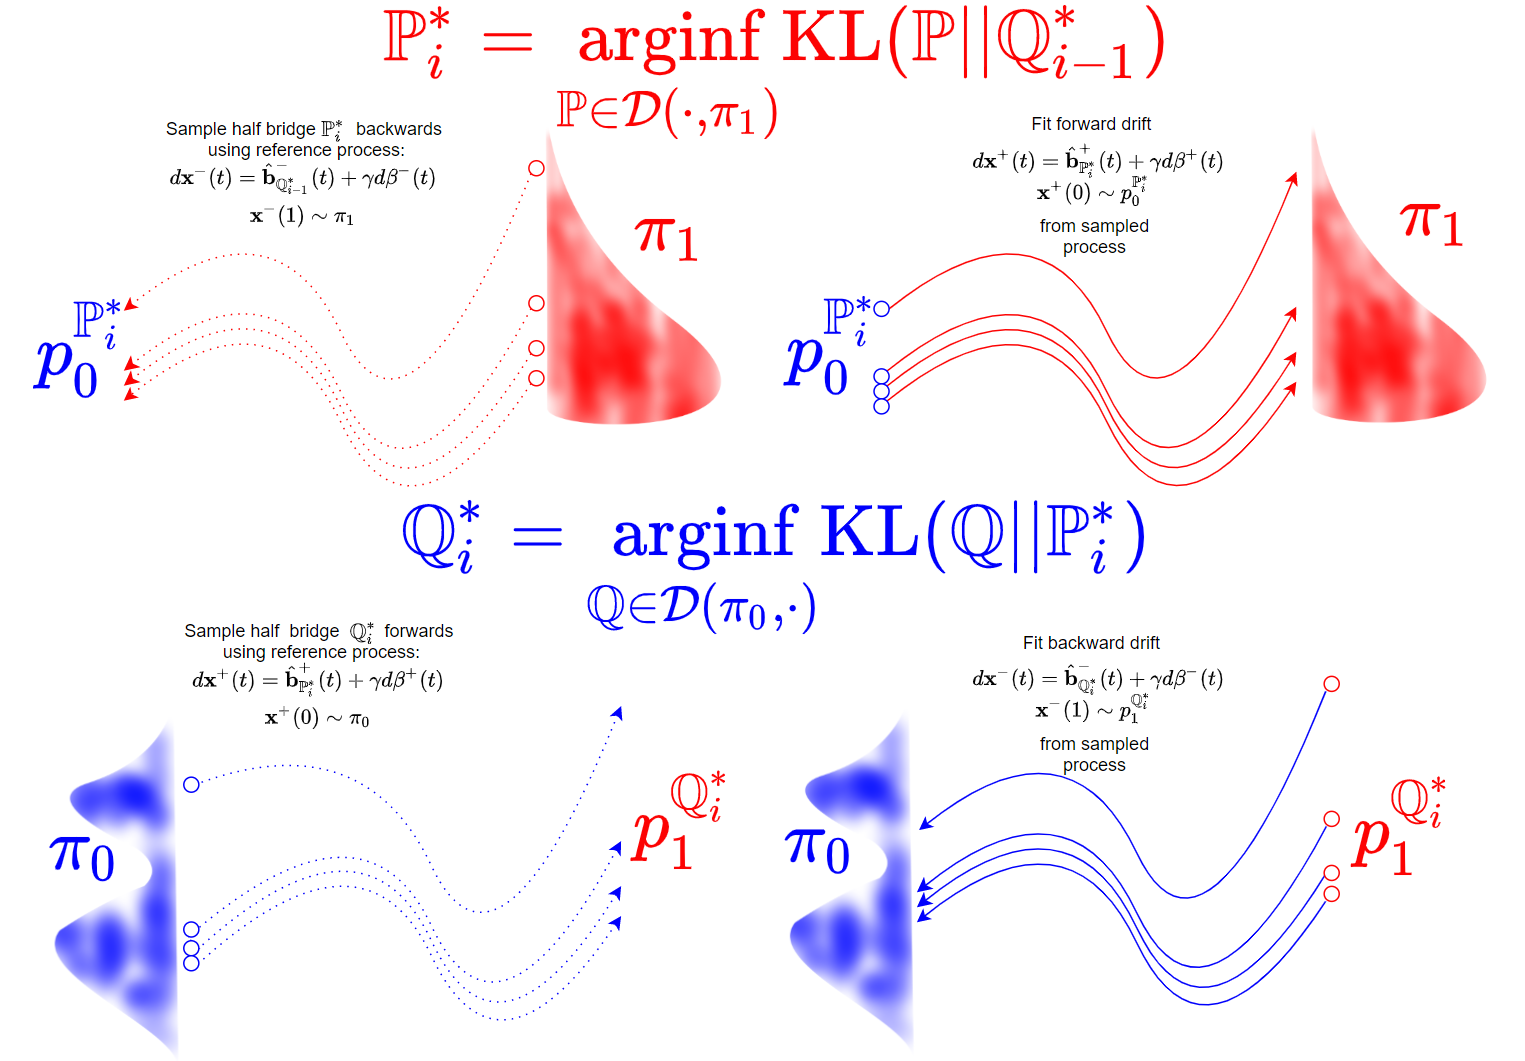
\includegraphics[scale=0.7]{images/gp_IPFP.PNG}
    \caption{$i^{\text{th}}$ Iteration for drift based approximation to g-IPFP. In each iteration, we draw samples from the process in the direction that incorporates the constraint as an initial value, and we learn the drift which simulates the same path measure in the opposite direction to the sampling. With each iteration $\mathbf{\color{blue}{p^{\P^{*}_i}_0}}$ and $\mathbf{\color{red}{p^{\Q^{*}_i}_1}}$ get closer to $\mathbf{\color{blue}{\pi_0}}$ and $\mathbf{\color{red}{\pi_1}}$ respectively.}
    \label{fig:gp_drift}
\end{figure}
\end{landscape}
and $K_d: \R^{d+1} \times \R^{d+1} \rightarrow \R$ is a valid kernel function. In practice, we are not making use of the predictive variances\footnote{We are effectively simply doing Kernel Ridge Regression.}. Instead, we simply use the predictive mean as an estimate of the drift and subsequently use that estimate to perform the EM method.

We now have the relevant ingredients to carry out this flavour of approximate g-IPFP specified in Algorithm  \ref{alg:gp_gipfp}, where the $\text{SDESolve}\Big(-\bar{\vb}^{-}_{\Q_{i-1}}, \gamma, \pi_1, \Delta t, M\Big)$ routine generates $M$ trajectories using the Euler-Mayurama method.

Note that we can use Equations \ref{eq:free_energy_1} and \ref{eq:free_energy_2}, which allow us to easily compute an estimate of the Schrödinger bridge using the current estimates of the optimal drifts.
%  $\{\vx^{+}_i(t_k)\}_{i,k}^N$ or  $\{\vx^{-}_j(t_l)\}_{j,l}^M$
\begin{algorithm} \label{alg:gp_gipfp}
\SetKwInOut{Input}{input}
\Input{$\pi_0(\vx), \pi_1(\vy), \W^{\gamma}$}
Initialise:\\
$i=0$ \\
$\Q^{*}_0 =\W^{\gamma}$\\
Obtain or estimate backward drift of prior: \\
$\bar{\vb}^{-}_{\Q_{0}}(\vx, t) := \text{ObtainBackwardDrift}(\Q^{*}_0)$\\

\Repeat{convergence}{
      $i := i + 1$ \\
      $\left\{\big(\vx^{-}_m(t_l)\big)_{l=0}^T\right\}_{m=0}^{M} = \text{SDESolve}\Big(-\bar{\vb}^{-}_{\Q_{i-1}}, \gamma, \pi_1, \Delta t, M\Big)$\\
     $ \bar{\vb}^{+}_{\P_{i}} := \text{GPDriftFit}\Big( \left\{\big(\vx^{-}_m(t_l)\big)_{l=0}^T\right\}_{m=0}^{M}, \gamma, \, \text{forward=True} \Big)$\\ 
     $\left\{ \big(\vx^{+}_n(t_k) \big)_{k=0}^T \right\}_{n=0}^{N} = \text{SDESolve}\Big(\bar{\vb}^{+}_{\P_{i}}, \gamma, \pi_0, \Delta t, N\Big)$ \\
     $\bar{\vb}^{-}_{\Q_{i}}\!:=\!\text{GPDriftFit}\Big(\! \left\{ \big(\vx^{+}_n(t_k) \big)_{k=0}^T \right\}_{n=0}^{N}, \gamma, \, \text{forward=False}\! \Big)$
    }
\Return{$\bar{\vb}^{-}_{\Q_{i}}, \bar{\vb}^{+}_{\P_{i}}$}
\caption{ Approximate g-IPFP with Gaussian processes (GP)   }
\end{algorithm}



\subsubsection{Sampling a Reverse-Time Diffusion }
A quick note to the reader is that the sign multiplying the drift in line $8$ of Algorithm \ref{alg:gp_gipfp} may seem arbitrary. However, we can motivate it by regarding an Itô-process as the continuous time limit of discrete time Markov chains.

We want to consider the case where both backward and forward transitions obey the same joint probability law, that is:
\begin{align}\label{eq:markov_e}
    p^{+}(\vx_{t+\Delta t}|\vx_t)p_t(\vx_t)=p^{-}(\vx_t|\vx_{t+\Delta t})p_{t+\epsilon}(\vx_{t+\Delta t}),
\end{align}
where $p_t(\cdot)$ is the marginal distribution at time $t$ and $p^{+}(\cdot|\cdot)$,  $p^{-}(\cdot|\cdot)$ respectively are Gaussians of the form:
\begin{align*}
p^{+}(\vx_{t+\Delta t}|\vx_t)&=\frac{1}{2\pi \Delta t }\exp\left(-\frac{1}{2\Delta t}\left[\vx_{t+\Delta t}-(\vx_t+\vb^{+}(\vx_t,t)\Delta t)\right]^2\right), \\
p^{-}(\vx_t|\vx_{t+\Delta t})&=\frac{1}{2\pi \Delta t}\exp\left(-\frac{1}{2\Delta t}\left[\vx_t-\left(\vx_{t+\Delta t}-\vb^{-}(\vx_{t+\Delta t},t+\Delta t)\Delta t\right)\right]^2\right).
\end{align*}
Taking logs on Equation \ref{eq:markov_e} and preserving a linear order in $\Delta t$ gives:
\begin{align*}
    (\vb^+(\vx_t,t)-\vb^-(\vx_{t+\Delta t},t+\Delta t)(\vx_{t+\Delta t}-\vx_t)=\log p_{t+\Delta t}(\vx_{t+\Delta t}) - \log p_t(\vx_t), 
\end{align*}
which in the continuous time limit arrives to our chosen flavour\footnote{Different authors (e.g. \cite{nagasawa2012stochastic}) parametrise the duality formula with different signs in turn changing the sign of the EM discretisation.} of Nelson's duality formula \citep{nelson1967dynamical}:
\begin{align*}
      \vb^+(\vx_t,t) -\vb^-(\vx_t,t) = \nabla\log p(\vx_t, t).
\end{align*}

\section{Stochastic Control Approach}

We would like to carry out a variant of g-IPFP that is based on the stochastic control formulations of the half bridge problems. Using a slight adaptation to Lemma \ref{lemma:control} we can rewrite the half bridge steps of g-IPFP as:
\begin{itemize}
\item Backward half bridge (time-reversed dynamics): 
\begin{align} \label{eq:controlled_haalf_bridge_forward}
  \rvb^{-}_{\P_{i}}(t) = \min_{\rvb^{-} \in \calB }  &\E_\P\left[\int_0^1 \frac{1}{2\gamma}\big|\big|\rvb^{-}(t) -\rvb^{-}_{\Q_{i-1}}(t), \big|\big|^2 dt\right] \nonumber \\
    s.t.\;\;\; d\rvx(t) = \rvb^{-}(t) &dt + \sqrt{\gamma} d\rvw^{-}(t), \;\; \rvx(1) \sim \pi_1.
\end{align}
\item Forward half bridge:
\begin{align} \label{eq:controlled_half_bridge_backward}
   \rvb^{+}_{\Q_{i}}(t) =\min_{\rvb^{+} \in \calB } & \E_\Q\left[\int_0^1 \frac{1}{2\gamma}\big|\big|\rvb^{+}(t) -\rvb^{+}_{\P_{i}}(t)\big|\big|^2 dt\right], \nonumber \\
    s.t.\;\;\; d\rvx(t) = \rvb^{+}(t) &dt + \sqrt{\gamma} d\rvw^{+}(t), \;\; \rvx(0) \sim \pi_0.
\end{align}.
\end{itemize}
The dual drifts can be obtained using Nelson's duality equations:
\begin{align*}
      \rvb^{-}_{\Q_{i-1}}(t)   &=\rvb^{+}_{\Q_{i-1}}(t) -\gamma\nabla_{\vx} p^{\Q_{i-1}}(\rvx(t), t) \\
    \rvb^{+}_{\P_{i}}(t) &=  \rvb^{-}_{\P_{i}}(t) +\gamma\nabla_{\vx} p^{\P_{i}}(\rvx(t), t).
\end{align*}
We express the dynamical evolution of $\P$ in the backward half bridge as a time reversed process \citep{pavon1991free, nelson1967dynamical}, such that the terminal distribution constraint $\rvx(1) \sim \pi_1$ becomes an initial value problem in reversed time, which is something we know how to sample from. 

In theory, we now have all the elements required to carry out g-IPFP under this control formulation. However, the dual drifts require the logarithmic gradient of the solution to their respective Fokker-Plank equations (i.e.\ $\nabla_{\vx} p^{\P_{i}}(\rvx(t), t)$, $\nabla_{\vx} p^{\Q_{i-1}}(\rvx(t), t)$). Estimating $p^{\P_{i}}(\rvx(t), t)$ or $p^{\Q_{i-1}}(\rvx(t), t)$ is very costly since we will also need to evaluate such estimations for every point in the interval $[0,1]$ that we use to estimate the integral $\int_0^1 \hdots dt$.

\subsection{Forward and Backward Diffusions}

As mentioned, Equations \ref{eq:controlled_half_bridge_backward}, and \ref{eq:controlled_haalf_bridge_forward} exhibit the computational challenge of estimating $p^{\X_{i}}(\rvx(t), t)$. In order to overcome this, we derive alternate expressions for Equations \ref{eq:controlled_half_bridge_backward} and \ref{eq:controlled_haalf_bridge_forward} that do not involve FPK solution terms inside the time integral.
\begin{proposition}\label{prop:halfforcontrol}
The forward half bridge (setting $\gamma=1$  for simplicity):
\begin{align*} 
   \rvb^{+}_{\Q_{i}}(t) =\min_{\rvb_\Q^{-} \in \calB } & \E_\Q\left[\int_0^1 \frac{1}{2}\big|\big|\rvb_\Q^{+}(t) -\rvb^{+}_{\P_{i}}(t)\big|\big|^2 dt\right], \nonumber \\
    s.t.\;\;\; d\rvx(t) = \rvb_\Q^{+}(t) &dt +  \rvw^{+}(t), \;\; \rvx(0) \sim \pi_0
\end{align*}
can be expressed as\footnote{We thank Professor Austen Lamacraft for providing the first sketch of this proof, which we have reviewed in detail and iterated on.}:
\begin{align} \label{eq:div_control_forward}
   \rvb^{+}_{\Q_{i}}(t) =\min_{\rvb^{-} \in \calB } -2\E_{p^{\Q}_1}\left[\log \pi_1 \right] &+ \E_{\Q}\left[\int_0^1 \left(\frac{1}{2}||\rvb_\Q^{+}(t) -\rvb_{\P_{i}}^{-}(t)||^2 - \nabla\cdot\rvb^{-}_{\P_{i}}(t) \right)\right], \nonumber \\
    s.t.\;\;\; d\rvx(t) = \rvb_\Q^{+}(t) &dt + \rvw^{+}(t), \;\; \rvx(0) \sim \pi_0.
\end{align}
\end{proposition}
\begin{proof}
We  abbreviate  terms of the form $p^{\X}(\rvx(t), t)$ with $p^{\X}_t$ and $\rvb^{\X}_{\pm}(t)$, using $\rvb^{\X}_{\pm}$ for compactness. We express the KL in terms of backward drifts (known result):
\begin{align}
\KL(\Q||{\P_{i}}) = \KL( p_0^{\Q}|| p_0^{{\P_{i}}}) + \frac{1}{2}\E_{\Q}\left[\int_0^1 || \rvb_\Q^{+} -\rvb_{\P_{i}}^{+}||^2 dt\right].
\end{align}
Using Nelson's duality formula $\rvb^{\P_{i}}_+(t) =\rvb^{\P_{i}}_-(t) + \nabla\log p_t$:
\begin{align}
\KL(\Q||{\P_{i}}) = \KL( p_0^{\Q}|| p_0^{{\P_{i}}}) + \frac{1}{2}\E_{\Q}\left[\int_0^1 || \rvb_\Q^{+} - \rvb_{\P_{i}}^{-} - \nabla\log p_t^{\P_{i}}||^2 dt\right].
\end{align}
Expanding:
\begin{align*}
\KL(\Q&||{\P_{i}}) = \KL( p_0^{\Q}|| p_0^{{\P_{i}}}) +\\ &\frac{1}{2}\E_{\Q}\left[\int_0^1 \left(|| \rvb_\Q^{+} - \rvb_{\P_{i}}^{-}||^2 - 2\nabla\log p_t^{\P_{i}} \cdot ( \rvb_\Q^{+} - \rvb_{\P_{i}}^{-}) + {\nabla\log p_t^{\P_{i}}}^2 \right)dt\right].
\end{align*}
Using the chain rule for the second derivative $\Delta \log  p = -\frac{(\nabla p)^2}{ p^2}  + \frac{\Delta  p}{ p}$:
\begin{align*}
&\KL(\Q||{\P_{i}}) =\KL( p_0^{\Q}|| p_0^{{\P_{i}}}) +\\ &\frac{1}{2}\E_{\Q}\left[\int_0^1 \left(\!\!|| \rvb_\Q^{+} - \rvb_{\P_{i}}^{-}||^2 \!\!- 2\nabla\log p_t^{\P_{i}}\!\!\!\cdot \!( \rvb_\Q^{+} - \rvb_{\P_{i}}^{-}) - \Delta \log  p^{\P_{i}}\!\!\!+ \frac{\nabla  p^{\P_{i}}}{ p^{\P_{i}}}\!\!\right)dt\right].
\end{align*}

Using Itô's rule, we can show the following: 
\begin{align*}
\E_\Q\left[\log p^{\P_{i}}_1-\log p^{\P_{i}}_0\right] = \E_\Q\left[\int dt \left(\rvb^+_\Q\cdot\nabla\log p_t^{\P_{i}} + \frac{1}{2}\Delta \log p_t^{\P_{i}}\right)\right],\\
\E_\Q\left[\int dt \left(\rvb_+^\Q\cdot\nabla\log p_t^{\P_{i}} \right)\right] = \E_\Q\left[\log p^{\P_{i}}_1-\log p^{\P_{i}}_0 - \int dt \left( \frac{1}{2}\Delta \log p_t^{\P_{i}}\right)\right].
\end{align*}

The above step is derived using Itô's formula:
\begin{align*}
d\log  p_t^{{\P_{i}}} =\rvb^+_\Q\cdot\nabla\log p_t^{\P_{i}} dt + \frac{1}{2}\Delta \log p_t^{\P_{i}} dt + \nabla \log p_t^{\P_{i}} \cdot d\rvw^{+}(t),
\end{align*}
which implies (taking expectations on both sides w.r.t. $\Q$ and then dividing by $dt$. See Equation 5.13, Theorem 5.4 from \cite{sarkka2019applied}):
\begin{align*}
\partial_t \E_{\Q}[\log  p_t^{{\P_{i}}}] = \E_{\Q}{\left[\rvb^+_\Q\cdot\nabla\log p_t^{\P_{i}} + \frac{1}{2}\Delta \log p_t^{\P_{i}}\right]}.
\end{align*}
Integrating both sides from $0$ to $1$ (and applying Fubini) gives the result.

Substituting this back into the KL (the Laplacians cancel out):
\begin{align*}
\KL(\Q||{\P_{i}}) = &\E_\Q\left[-\log \frac{ p^{\P_{i}}_1}{ p^\Q_0}\right] \\+ &\frac{1}{2}\E_{\Q}\left[\int_0^1 \left(|| \rvb_\Q^{+} - \rvb_{\P_{i}}^{-}||^2 + 2\nabla\log p_t^{\P_{i}} \cdot \rvb_{\P_{i}}^{-}+ \frac{\Delta  p^{\P_{i}}}{ p^{\P_{i}}}\right)dt\right].
\end{align*}
Since $ p_t^{\P_{i}}$ obeys the Fokker-Planck equation (this is the case for diagonal covariance Itô-Processes, otherwise we would have cross terms from the Hessian, see Equation 13.4 in \cite{nelson1967dynamical}\footnote{more generally we have $\pm\partial_t p_t^{\P_{i}} = \frac{1}{2}\Delta p_t^{\P_{i}}\mp\nabla\cdot(\rvb_\pm^{\P_{i}} p_t^{\P_{i}})$}): 
\begin{align*}
-\partial_t p_t^{\P_{i}} = \frac{1}{2}\Delta p_t^{\P_{i}}+\nabla\cdot(\rvb_{-}^{\P_{i}} p_t^{\P_{i}}).
\end{align*}
Using the product rule: 
\begin{align*}
-\partial_t p_t^{\P_{i}} = \frac{1}{2}\Delta p_t^{\P_{i}}+  p_t^{\P_{i}} \nabla\cdot(b_{-}^{\P_{i}}) + \rvb^{-}_{\P_{i}} \cdot \nabla p_t^{\P_{i}}, \\
-\partial_t p_t^{\P_{i}} -  p_t^{\P_{i}} \nabla\cdot \rvb^{-}_{\P_{i}}  = \frac{1}{2}\Delta p_t^{\P_{i}}+ \rvb^{-}_{\P_{i}} \cdot\nabla  p_t^{\P_{i}}.
\end{align*}
Dividing both sides by $ p_t^{\P_{i}}$:
\begin{align*}
-\partial_t \log  p_t^{\P_{i}} - \nabla\cdot \rvb^{-}_{\P_{i}}  = \frac{1}{2}\frac{\Delta  p_t^{\P_{i}}}{ p_t^{\P_{i}}}+  \rvb^{-}_{\P_{i}} \cdot \nabla \log  p_t^{\P_{i}}.
\end{align*}
Substituting back into the KL we have:
\begin{align*}
\KL(\Q||{\P_{i}}) &= \E_\Q\left[-\log \frac{{ p^{\P_{i}}_1}^2}{ p^\Q_0  p_0^{{\P_{i}}}}\right] + \frac{1}{2}\E_{\Q}\left[\int_0^1 \left(|| \rvb_\Q^{+} - \rvb_{\P_{i}}^{-}||^2 - 2\nabla\cdot \rvb^{-}_{\P_{i}} \right)dt\right], %\\
%\KL(\Q||{\P_{i}}) &= \E_\Q\left[-\log \frac{{ p^{\P_{i}}_1}^2}{ p^\Q_0   p_0^{{\P_{i}}}}\right] + \E_{\Q}\left[\int_0^1 \left(\frac{1}{2}|| \rvb_\Q^{+} - \rvb_{\P_{i}}^{-}||^2 - \nabla\cdot \rvb^{-}_{\P_{i}} \right)dt\right].
\end{align*}
We are only interested in terms that depend on $\rvb^{+}_\Q$ for the optimisation. Using that $p^{\P_{i}}_1=\pi_1$, which follows as a constraint from the previous iteration, we arrive at:
\begin{align}
\KL(\Q||{\P_{i}}) \propto -2\E_{ p^\Q_1}\left[\log {{ \pi_1 }} \right] + \E_{\Q}\left[\int_0^1 \left(\frac{1}{2}|| \rvb_\Q^{+} - \rvb_{\P_{i}}^{-}||^2 - \nabla\cdot \rvb^{-}_{\P_{i}} \right)dt\right].
\end{align}
\end{proof}
Following the same steps as above, we derive the equivalent result for the backward bridge.
\begin{proposition}
The backward half bridge:
\begin{align*} 
   \rvb^{-}_{\P_{i}}(t) =\min_{\rvb_{\P}^{-} \in \calB } & \E_\Q\left[\int_0^1 \frac{1}{2}\big|\big|\rvb_\P^{-}(t) -\rvb^{-}_{\Q_{i-1}}(t)\big|\big|^2 dt\right], \nonumber \\
    s.t.\;\;\; d\rvx(t) = \rvb_\P^{-}(t) &dt +  \rvw^{-}(t), \;\; \rvx(1) \sim \pi_1,
\end{align*}
can be expressed as:
\begin{align} \label{eq:div_control_backward}
   \rvb^{+}_{\P_{i}}(t) =\min_{\rvb_\P^{-} \in \calB } -2\E_{p^{\P}_0}\left[\log \pi_0 \right] &+ \E_{\P}\left[\int_0^1 \left(\frac{1}{2}||\rvb_\P^{-}(t) - \rvb_{\Q_{i-1}}^{+}(t)||^2 + \nabla\cdot\rvb^{+}_{\Q_{i-1}}(t) \right)\right], \nonumber \\
    s.t.\;\;\; d\rvx(t) = \rvb_\P^{-}(t) &dt +  \rvw^{-}(t), \;\; \rvx(1) \sim \pi_1.
\end{align}.
\end{proposition}
We now have all the ingredients to carry out g-IPFP using the newly derived half bridge formulations:
\begin{itemize}
    \item Backward step:
    \begin{align*}
   \rvb^{+}_{\P_{i}}(t) =\min_{\rvb_\P^{-} \in \calB } -2\E_{p^{\P}_0}\left[\log \pi_0 \right] &+ \E_{\P}\left[\int_0^1 \left(\frac{1}{2}||\rvb_\P^{-}(t) - \rvb_{\Q_{i-1}}^{+}(t)||^2 + \nabla\cdot\rvb^{+}_{\Q_{i-1}}(t) \right)\right], \nonumber \\
    s.t.\;\;\; d\rvx(t) = \rvb_\P^{-}(t) &dt + \sqrt{\gamma} \rvw^{-}(t), \;\; \rvx(1) \sim \pi_1.
    \end{align*}
    \item Forward step:
    \begin{align*} 
   \rvb^{+}_{\Q_{i}}(t) =\min_{\rvb^{+} \in \calB } -2\E_{p^{\Q}_1}\left[\log \pi_1 \right] &+ \E_{\Q}\left[\int_0^1 \left(\frac{1}{2}||\rvb_\Q^{+}(t) - \rvb_{\P_{i}}^{-}(t)||^2 - \nabla\cdot\rvb^{-}_{\P_{i}}(t) \right)\right], \nonumber \\
    s.t.\;\;\; d\rvx(t) = \rvb_\Q^{+}(t) &dt + \sqrt{\gamma} \rvw^{+}(t), \;\; \rvx(0) \sim \pi_0.
    \end{align*}
\end{itemize}
Here, $\rvb^{+}_{\Q^{0}}(t)$  is initialised in accordance to the prior (such that $\Q^0=\W^\gamma$), which in the case of Brownian $\W^\gamma$ motion is zero, that is $\rvb^{+}_{\Q_{0}}(t) =0$.

We highlight that the newly derived objective has an interpretable  decomposition:
\begin{align*}
 \mathcolor{blue}{\overbrace{-2\E_{p^{\P}_0}\left[\log \pi_0 \right]}^{\textbf{cross entropy/data fit}}} &+ \mathcolor{red}{\overbrace{\E_{\P}\left[\int_0^1 \left(\frac{1}{2}||\rvb_\P^{-}(t) - \rvb_{\Q_{i-1}}^{+}(t)||^2 + \nabla\cdot\rvb^{+}_{\Q_{i-1}}(t) \right)\right] }^{\textbf{path error}}}.
\end{align*}

The $\mathcolor{blue}{\textbf{cross entropy/data fit}}$ term acts a density estimator encouraging the drift to match its end point distribution, in this case $\mathcolor{blue}{\pi_0}$. Meanwhile, the $\mathcolor{red}{\textbf{path error}}$ term enforces the duality of the drifts, as well as making the process akin to the reference prior in the KL sense.

Note that the new terms left to estimate that may seem nontrivial are the cross entropy terms $\E_{p^{\Q}_1}\left[\log \pi_1 \right]$ and $\E_{p^{\P}_0}\left[\log \pi_0 \right]$. We will later discuss how to estimate the cross entropy of two distribution that are only available through samples. 

\subsection{Numerical Implementation}

The objectives we have just derived are in general not solvable in closed form for the optimal drift, thus we will require three main approximations:
\begin{itemize}
    \item A parametrisation of the drift such that we can optimise the objectives approximately using gradient based methods.
    \item A Monte Carlo approximation to the path integrals arising from the expectations.
    \item We need to be able to estimate the cross entropy terms as discussed previously.
\end{itemize}

We proceed to discuss these approximations in more detail.
\subsubsection{Numerical Optimization (Differentiable Parametrisation)}

In order to optimise the control based variants of the half bridge objectives, we need to parametrise the drift as a differentiable function \footnote{We could alternatively parametrise the space of admissible control signals $\calB$ as a functional space (i.e.\ an  RKHS \citep{alvarezkernel}) in which we may be able to carry out minimisation of the half bridges in closed form.}. We parametrise the forward and backward drift with neural networks:
\begin{align} \label{eq:drift_param}
    \rvb^{+}_{\Q}(t) := \rvb^{+}_{\phi}(\vx(t), t), \nonumber \\
    \rvb^{-}_{\P}(t) := \rvb^{-}_{\theta}(\vx(t), t).
\end{align}
Rather than optimising over $\calB$, the optimisations are carried out in terms of the parameters $\theta$ and $\phi$ respectively. This will also help in the next step, which is estimating the expectations and integrals in the half bridge objective.

We refer to the path measures induced under this parametrisation as $\P_{\theta}$ and $\Q_{\phi}$ respectively.

\subsubsection{Numerical Integration (Path Error Term)}
We can sample from $\Q_{\phi}$ and $\P_{\theta}$, whilst enabling the single boundary constraints using the Euler-Mayurama method:
\begin{itemize}
    \item  Forward SDE discretisation for $\Q_{\phi}$:
\begin{align*}
    \rvx_{t + \Delta t} = \rvx_t + \rvb^{+}_{\phi}(\vx_t, t) + \sqrt{\gamma} \rvepsilon, \quad \rvx_0 \sim \pi_0, \;\;\rvepsilon \sim \calN(\vzero, \I).
\end{align*}
    \item  Backward SDE discretisation for $\P_{\theta}$:
\begin{align*}
    \rvx_{t} = \rvx_{t+\Delta t} - \rvb^{-}_{\phi}(\vx_t, t) + \sqrt{\gamma} \rvepsilon, \quad \rvx_1 \sim \pi_1,\;\; \rvepsilon \sim \calN(\vzero, \I).
\end{align*}
\end{itemize}

Once we have sampled batches of trajectories $\{\vx^{+}_i(t_k)\}_{n,k}^N$ and $\{\vx^{-}_j(t_l)\}_{m,l}^M$, we can proceed to estimate the path error term in the objective using the Monte Carlo  method:


\begin{itemize}
    \item Backward path error term 
\begin{align}
    \E&_{\P}\left[\int_0^1 \left(\frac{1}{2}||\rvb_\P^{-}(\vx(t),t) - \rvb_{\Q_{i-1}}^{+}(\vx(t),t)||^2 + \nabla\cdot\rvb^{+}_{\Q_{i-1}}(\vx(t),t) \right)\right] \approx \nonumber   \\
    &\frac{\Delta t}{M} \sum_{m,l}\left(\frac{1}{2}||\rvb_\phi^{-}(\vx^{-}_m(t_l), t_l) - \rvb_{\theta}^{+}(\vx^{-}_m(t_l), t_l)||^2 + \nabla\cdot\rvb^{+}_{\theta}(\vx^{-}_m(t_l), t_l)\right).
\end{align}
    \item Forward path error term
\begin{align}
    \E&_{\Q}\left[\int_0^1 \left(\frac{1}{2}||\rvb_\Q^{+}(\vx^{-}(t), t) - \rvb_{\P_{i}}^{-}(\vx, t)||^2 - \nabla\cdot\rvb^{-}_{\P_{i}}(\vx, t) \right)\right]  \approx \nonumber   \\
    &\frac{\Delta t}{N} \sum_{n,k}\left(\frac{1}{2}||\rvb_\theta^{+}(\vx^{+}_n(t_k), t_k) - \rvb_{\phi}^{-}(\vx^{+}_n(t_k), t_k)||^2 - \nabla\cdot\rvb^{-}_{\phi}(\vx^{+}_n(t_k), t_k)\right).
\end{align}
\end{itemize}
\subsubsection{Cross-entropy Boundary Terms}

The densities inside the cross-entropy terms are $\pi_0, \pi_1$, which we only have access to via samples. Thus, we can not apply the standard Monte Carlo  method as we can not evaluate the integrands $\pi_0, \pi_1$ at the Monte Carlo samples.

Therefore, we are required to use some form of density estimation for the boundary distributions $\pi_0, \pi_1$, in order to compute a Monte Carlo  estimator for the cross entropy boundary terms. The two approximations we consider are non parametric approximations using Kernel Density Estimation and K-Nearest Neighbours.

We need to estimate:
\begin{align*}
\E_{\pi_0^\P}[\ln\pi_{0}] &\approx \frac{1}{M}\sum_{m}^{M} \ln \hat{\pi}_0(\vx_m^{-}(1)), \\
\E_{\pi_1^\Q}[\ln\pi_{1}] &\approx \frac{1}{N}\sum_{n}^{N} \ln \hat{\pi}_1(\vx_n^{+}(0)),
\end{align*}
where $\hat{\pi}_i$ is a KDE based approximation of $\pi_i$:
\begin{align*}
\hat{\pi}_0(\vx) = \frac{1}{N} \sum_n^{N} \kk_{\mH_x}(\vx - \vx_n), \\
\hat{\pi}_1(\vy) = \frac{1}{M} \sum_m^{M} \kk_{\mH_y}(\vy - \vy_m),
\end{align*}
where $\kk_{\textbf{H}}$ is a smooth function called a kernel. In our case, we use the Squared Exponential kernel:
\begin{align*}
\kk_{\mH}(\vx-\vx') = (2\pi)^{d/2}|\mH|^{-1/2}\exp\left(-\frac{1}{2}||\vx-\vx'||^{2}_{\mH^{-1}}\right),
\end{align*}
where the bandwidth matrix $\mH$ is set using Silverman's rule \citep{silverman1986density}:
\begin{align}
\mH_{ij} = \begin{cases}
\left(\frac{4}{d+2}\right)^{\frac{2}{d+4}} N^{\frac{-2}{d+4}} \sigma_{i}^2  &\text{  if  } i=j, \\
0  &\text{otherwise},
\end{cases}
\end{align}

where $N$ is the number of data points used in the KDE estimate. Alternatively, for estimating the densities non-parametrically one can use a K-nearest neighbours basis \citep{veksler2013nonparametric}:
\begin{align*}
\hat{\pi}_0(\vx) \propto  \text{R}_k(\vx, \{\vx_n\})^{-d}\\
\hat{\pi}_1(\vy) \propto \text{R}_k(\vy, \{\vy_m\})^{-d},
\end{align*}
where $\text{R}_k(\vx, \{\vx_i\})$ is the distance to the $k^{th}$ nearest neighbour of $\vx$ in $\{\vx_i\}$.  Approximating the density with a KNN basis is the core ingredient for approximating entropy in \cite{singh2016analysis}.

\subsection{Mode Collapse in Reverse KL}

\begin{figure}
    \centering
    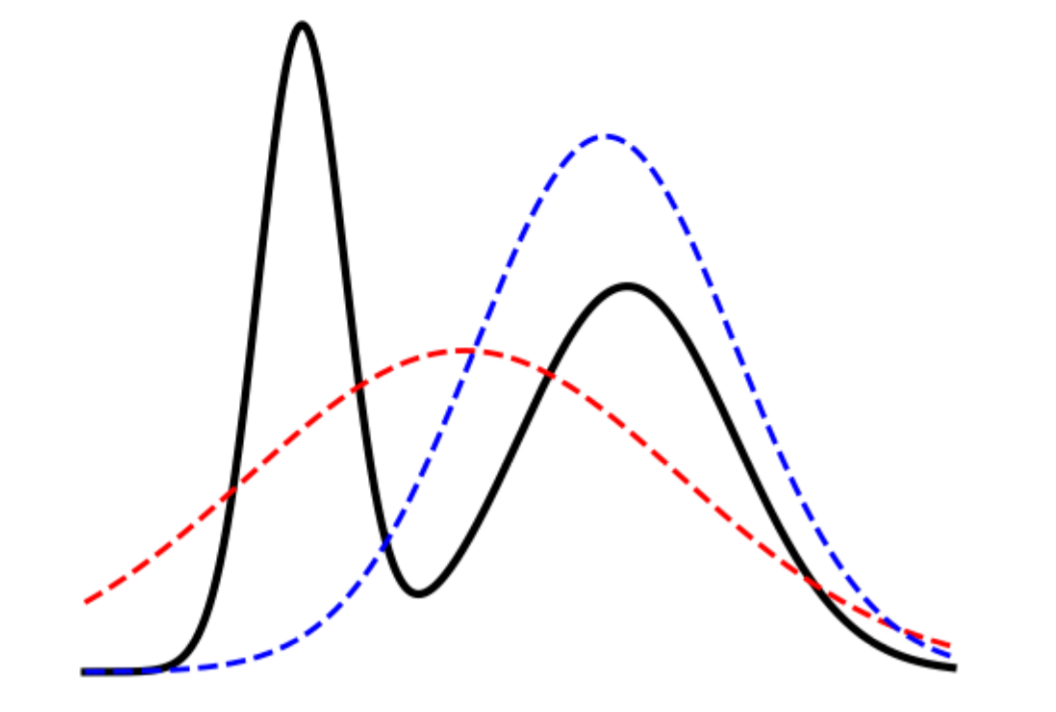
\includegraphics[scale=0.5]{images/zhang_et_al.PNG}
    \caption{Figure 1 from \cite{zhang2019variational}:  Fitting a Gaussian to a mixture of Gaussians (black) by
minimizing the forward KL (red) and the reverse KL (blue).}
    \label{fig:babrber_kl}
\end{figure}

The forward KL (e.g. Maximum Likelihood)  $\argmin_{\Q \in \cdot }\KL(\P ||\Q)$  blows up  when $\P$ tries to assign $0$ to regions where $\Q$ has mass. The reverse KL (i.e $\argmin_{\Q }$ $\KL(\Q ||\P)$) can be prone to mode collapse \citep{zhang2019variational}. The issue arises from the expectations and minimisations both being taken with respect to $\Q$. Thus we can set the measure $\Q$ to 0 for regions where $\P$ has mass without incurring in an additional penalty since this zeroes out the cost over that region.

As put succinctly in \cite{lawrence2001variational}:

\textit{"In other words, when the approximating distribution is not
well matched to the true posterior, the former case is likely to produce a very implausible inference.
The latter case will only produce plausible inference, in legal terms it would find the truth, nothing
but the truth, but not the whole truth."}

Meaning that the reverse KL provides us with the truth (it is precise), yet  it does not provide us with the whole truth (i.e. has low recall).

\section{Conceptual Comparison of Approaches}

In this section we briefly define and contrast some of the points of failure of each method based on conceptual observations prior to any experimentation.

\begin{table}[]
\caption{Challenges faced by methods. A check mark indicates the method overcomes the respective pitfall.}\label{tab:conceptual_pits}
\begin{adjustbox}{width=\columnwidth}
\begin{tabular}{LllllF}
\toprule
\multirow{3}{*}{Method} & Copes with                  & No            & Handles                & Scales well          & No Explicit              \\
                        & Mode              &  Auxiliary           & Distant               & in $N,M$              & Density               \\
                        &  Collapse                     &    Sampling                     & Support               & and $\Delta t$        & Estimation            \\ \midrule
\cite{pavon2018data}      & \cmark & \xmark & \xmark & \cmark & \xmark \\
Drift Estimation & \cmark & \cmark & \xmark & \xmark                 & \cmark  \\ 
Stochastic Control      & \xmark & \cmark & \cmark & \cmark & \xmark \\
\bottomrule
\end{tabular}
\end{adjustbox}
\end{table}
\begin{itemize}
    \item \textbf{Copes with Mode Collapse}: This occurs when the optimisation procedure is not penalised for missing a particular mode in the boundary distributions. As a result the method is prone to missing modes and is unable to map between distributions with a signficant difference in the numbers of modes.
    \item \textbf{No Auxiliary Sampling:} This is concerned with computing integrals with auxiliary distributions (e.g. importance sampling) as done in the method by \cite{pavon2018data}.
    \item \textbf{Handles Distant Support:} This issue is concerned with being unable to generate samples that are in the empirical support of $\pi_1$ when evolving from $\pi_0$ (and vice-versa). This problem is due to the reference process not being able to transport samples from one marginal to areas where there is mass in the other marginal. As a result, this will not give any initial signal to the IPFP algorithm and in lay terms it will not kick off the feedback-loop that refines the constraints in turn.
    \item \textbf{Scales well in $N,M$ and $\Delta t$:} By this we mean that the method scales well in the number of data-points, a problem with most non-parametric kernel methods that are $\mathcal{O}((NM\Delta t)^2)$ in memory and $\mathcal{O}((N M\Delta t)^3)$ in computation. Note that there are techniques to overcome this (e.g.\ sparse variational approaches \citep{van2019sparse}).
    \item \textbf{No Explicit Density Estimation:} This applies to methods that require solving an explicit density estimation task at each g-IPFP iteration. Whilst not a major downside,  \cite{pavon2018data} mentions that density estimation in high dimensions may be both difficult and inaccurate, resulting in poor g-IPFP iterations.
\end{itemize}
We believe that mode collapse  and auxiliary sampling are the most impact-full issues when numerically solving the empirical bridge, since there are mitigations for the other issues. We could not find any successful heuristics to improve mode collapse. For auxiliary sampling based approaches as in \cite{pavon2018data}, it becomes very difficult to scale them to high dimensions. In particular, one needs to design an approach that is aware of where the mass in the integrand resides, as in \cite{osborne2012active}. This is where our proposed methods have the biggest advantage.
\\The problem of missing the support of the boundary distributions can be addressed by re-scaling the data (i.e. standardise) so that it is at a scale where the Brownian motion prior can cover the support of the boundaries when going from one to the other. Alternatively, increasing the value of $\gamma$ will also achieve this. See Table \ref{tab:conceptual_pits} for a conceptual comparison between the studied methods in this thesis.

\section{Summary}

In this section we studied and proposed different approaches for numerically solving the Schrödinger bridge problem. Since the algorithms used for solving the Schrödinger bridge are derived from the g-IPFP framework, much of the focus in this chapter is placed on how to solve the half bridges numerically, given these are the inner steps of the g-IPFP based algorithms. 

\begin{itemize}
    \item Presented the method by \cite{pavon2018data} for solving the  Schrödinger system via a maximum likelihood variant of Fortet's. This method proposes representing the potentials in the Schrödinger system as parametric functions and enforces the steps in Fortet's algorithm using maximum likelihood.
    \item Introduced a novel direct drift estimation based approach using Gaussian processes. This method proposes to approximate the optimal half bridge path measures directly by fitting a dual drift to trajectories sampled from the optimal half bridge path measure. We use the method by \cite{ruttor2013approximate} in order to fit the drift of an SDE observed through samples.
    \item Introduced a novel approach for solving the dynamic half bridges numerically using the stochastic control formulation of the half bridges. In this approach we represent the drift as a parametric function and numerically minimise the half bridge objective with respect to the drifts parameters. 
    \item Presented a conceptual comparison of the 3 discussed approaches , discussing their strengths and weakness. 
\end{itemize}
%\chapter{Evaluation} 
\chapter{Experiments}

In this section we explore the performance of our methods for the empirical Schrödinger bridge on toy 1D and 2D datasets. We limit to toy data which we can visually evaluate, due to the early nature of the approaches. This helps gainining a practical understanding of their mechanics and limitations before handling real world data. 

Our experiments can be grouped into the following tasks:
\begin{itemize}
    \item \textbf{Unimodal to Unimodal Tests:} In these experiments we evaluate the ability of the algorithms to transition from simple unimodal Gaussian distributions with different means and variances. This is one of the simplest tests and serves as the most basic sanity check for each method.
    \item \textbf{Unimodal to Multimodal Tests:} Some of the methods might suffer from mode collapse. In order to evaluate the ability of a method to fit multimodal boundaries, we set up a simple test of mapping from a unimodal distribution to a multimodal one. 
    \item \textbf{Non-Gaussian Distributions Tests:} Here we explore the tasks for mapping from a unimodal Gaussian to a complex non-Gaussian distribution, such as the moons and circles datasets \cite{pedregosa2011scikit}. Due to time constraints, we only explored this test with the direct drift estimation approach.
\end{itemize}

Finally, we select two toy datasets (one unimodal to unimodal and one unimodal to bimodal) which all methods managed to fit visually, and construct a hypothesis test for comparing the methods against each other in a more statistically sound framework.  We have open-sourced the code for the experiments and algorithms \footnote{For our proposed approach the experiments can be found at \url{https://github.com/franciscovargas/SC-IPFP/tree/master/SC_IPFP/torch/final_notebooks}. For the experiments with the method by \cite{pavon2018data} the notebooks can be found at \url{https://github.com/franciscovargas/DataDrivenSchrodingerBridge/tree/master/notebooks}}.
\begin{figure}[t]
    \centering
    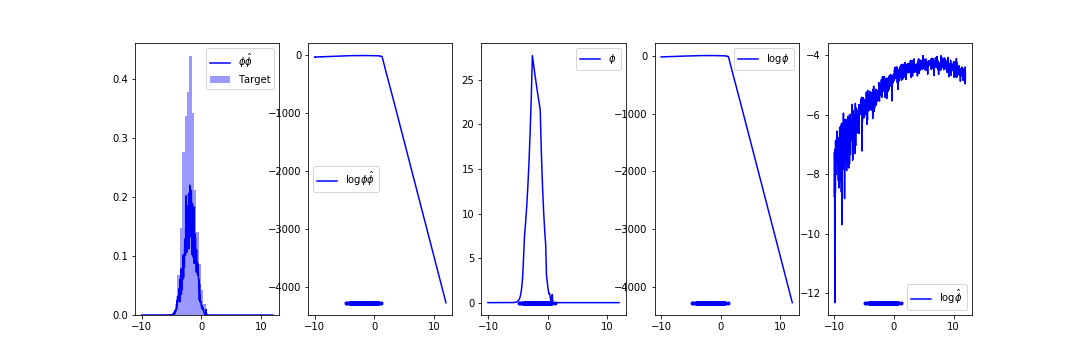
\includegraphics[scale=0.4,trim={2.3cm 0.2cm 1.5cm 0}, clip]{images/Pavon/Forward_unimodal_working_pavon_relu_nn500.png}\\\vspace{-0.2cm}
    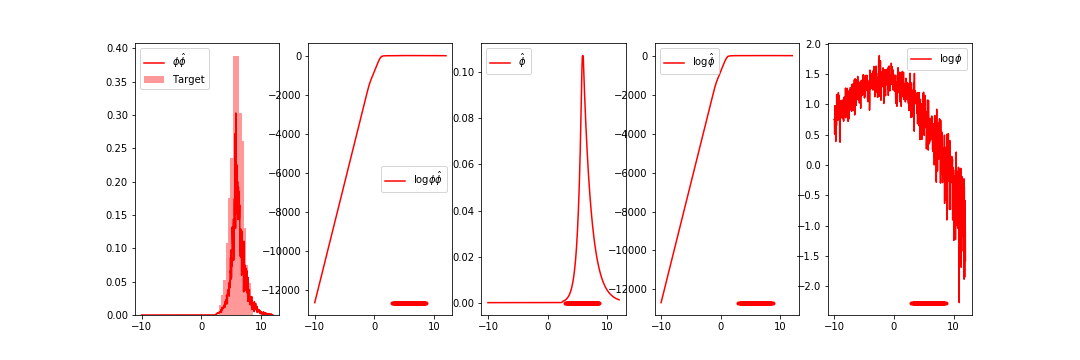
\includegraphics[scale=0.4,trim={2.3cm 0 1.5cm 1.5cm}, clip]{images/Pavon/Backward_unimodal_working_pavon_relu_nn500.png} 
    \caption{Schrödinger Bridge results using the method by \cite{pavon2018data} on unimodal Gaussian 1D data. We included the potentials since it was helpful to illustrate how they compensate each other. }
    \label{fig:driftpavon}
\end{figure}

\section{Method by \cite{pavon2018data}}
\begin{figure}[t]
    \centering
    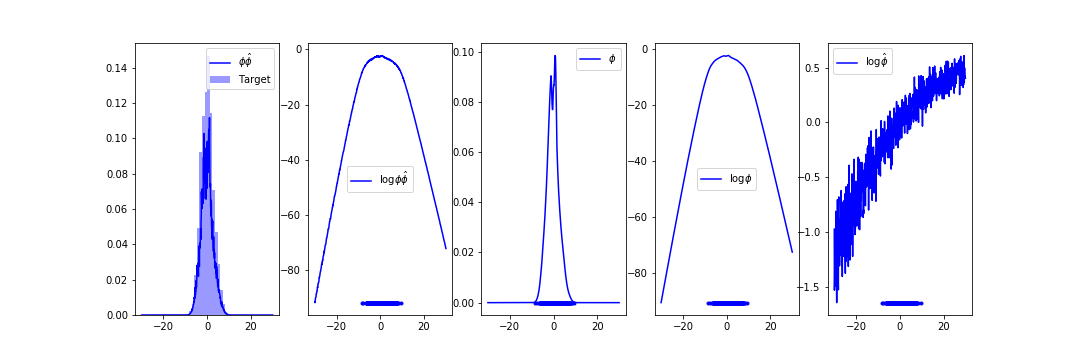
\includegraphics[scale=0.4,trim={2.3cm 0.2cm 1.5cm 0}, clip]{images/Pavon/Forward_bigvar_test_working.png}\\\vspace{-0.2cm}
    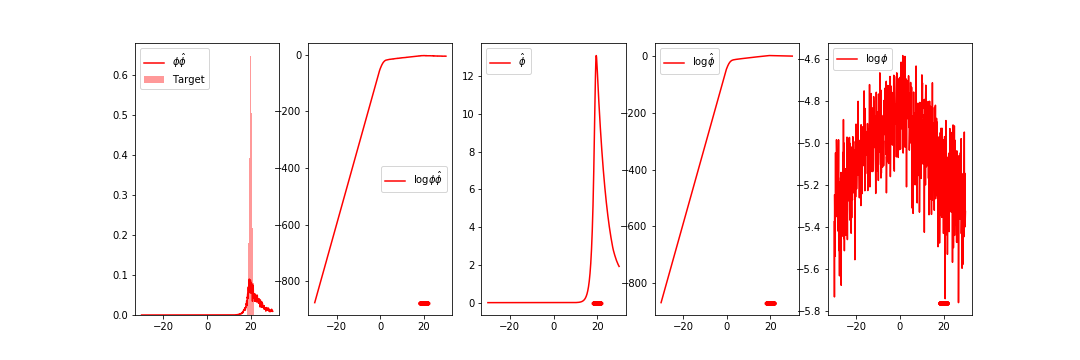
\includegraphics[scale=0.4,trim={2.3cm 0 1.5cm 1.5cm}, clip]{images/Pavon/Backward_bigvar_test_working.png} 
    \caption{Schrödinger Bridge results using the method by \cite{pavon2018data} on unimodal Gaussian 1D data and different variances. }
    \label{fig:small_to_big}
\end{figure}
We found \cite{pavon2018data} to be extremely sensitive to the value of $\gamma$ in the prior $\W^{\gamma}$: for most values of $\gamma < 5$, the method worked poorly and the boundary distributions would collapse to Dirac delta distributions. In order to overcome this issue, we had to experiment with large values of $\gamma$. Alternatively, we found that another heuristic to overcome this issue was to standardise the data.  This led us to understand that the issue was due to not being able to cover the support of the boundary distributions when sampling from the transition density of $\W^{\gamma}$. 

We set $\gamma=1000$ in all the following experiments, unless stated otherwise. We determined this value to be stable enough for us to explore the method. We used $400$ Monte Carlo  samples for each of the expectations approximated. A single hidden layer neural network \citep{lecun2015deep} with ReLu activations \citep{glorot2011deep} with $500$ hidden units is used to parametrise the potentials across all experiments. We used Glorot initialisation \citep{glorot2010understanding} to initialize the weights and the optimizer was Adagrad \citep{duchi2011adaptive}.  Each example was trained for an outer loop of $250$ epochs with $150$ inner epochs for the MLE sub-iterations. 
\begin{figure}
    \centering
    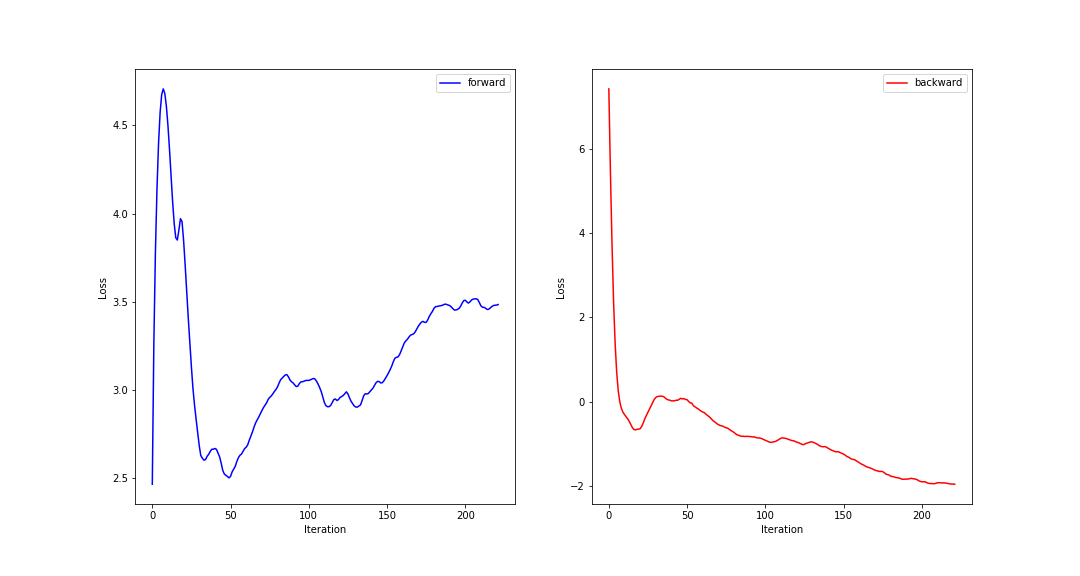
\includegraphics[scale=0.4,trim={2.3cm 1cm 2.5cm 0}, clip]{images/Pavon/pavon convergence big var.png} \vspace{-0.6cm}
    \caption{Likelihood per epoch for the method by \cite{pavon2018data} applied to unimodal Gaussian 1D data with different variances. }
    \label{fig:small_to_big_convergence}
\end{figure}
\subsection{Unimodal Experiments}

In this section, we explore transitioning from two normal distributions with different means and variances. We also illustrate how the method fails for small values of $\gamma$ and correctly diagnose a cause, in addition to proposing heuristics to overcome this issue. 

\subsubsection{Different Means, Same Variances}

In this experiment, we explore the following generative process for the marginals:
\begin{align*}
\color{blue}{\pi_0(x)} &\color{blue}{= \calN(x; 5,  1)} \\
    \color{red}{\pi_1(y)} &\color{red}{= \calN(y; -2, 1)}. 
\end{align*}
Results can be found in Table \ref{fig:driftpavon}, where we visually observe a good fit of the boundary distributions. This experiment serves mostly as a sanity check and to tune $\gamma$ to a value where the method is stable.

\begin{figure}[t]
    \centering
    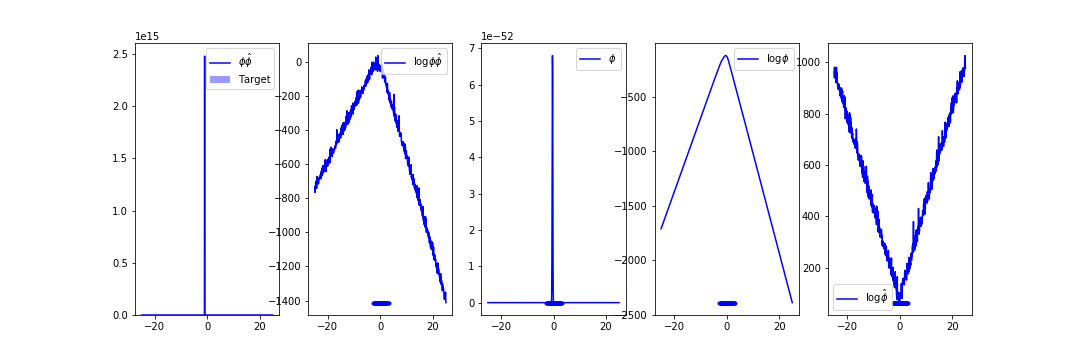
\includegraphics[scale=0.4,trim={2.3cm 0.2cm 1.5cm 0}, clip]{images/Pavon/Forward_unimodal_test_working_convex.png} \\\vspace{-0.2cm}
    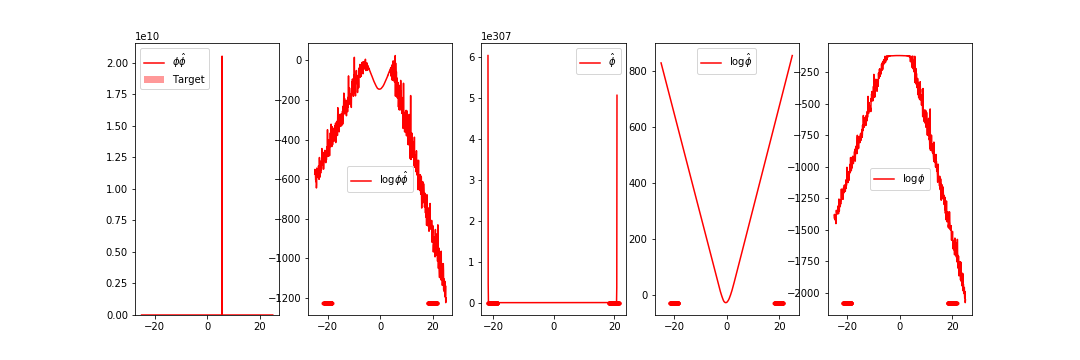
\includegraphics[scale=0.4,trim={2.3cm 0 1.5cm 1.5cm}, clip]{images/Pavon/Backward_unimodal_test_working_convex.png} 
    \caption{Schrödinger Bridge results using the method by \cite{pavon2018data} on unimodal to bimodal Gaussian 1D data. This example illustrates the Dirac delta collapse of the marginals.}
    \label{fig:small_delta_collapse}
\end{figure}
\subsubsection{Different Means and Variances}

We generated a 1D toy dataset using the following process:
\begin{align*}
     \color{blue}{\pi_0(x)} &\color{blue}{= \calN(x; 0,  9)} \\
    \color{red}{\pi_1(y)} &\color{red}{= \calN(y; 20, 0.5 ^2)}. 
\end{align*}
Results can be found in Figure \ref{fig:small_to_big}, where we observe a good fit for $\color{blue}{\pi_0}$, yet visually not such a good fit for $\color{red}{\pi_1}$. Furthermore, the Lagrange constraint integral converged to approximately $0.6$ rather than $1$, meaning the distribution was not normalised via this approximate Lagrange multipliers based approach. From Figure \ref{fig:small_to_big_convergence} it is not clear if the method fully converged. 
\begin{figure}[t]
    \centering
     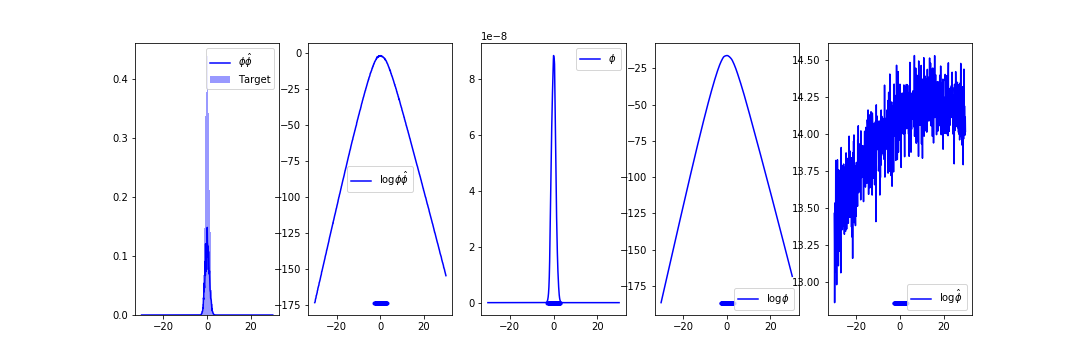
\includegraphics[scale=0.4,trim={2.3cm 0.2cm 1.5cm 0}, clip]{images/Pavon/Forward_bimodal_test_working.png} \\ \vspace{-0.2cm}
    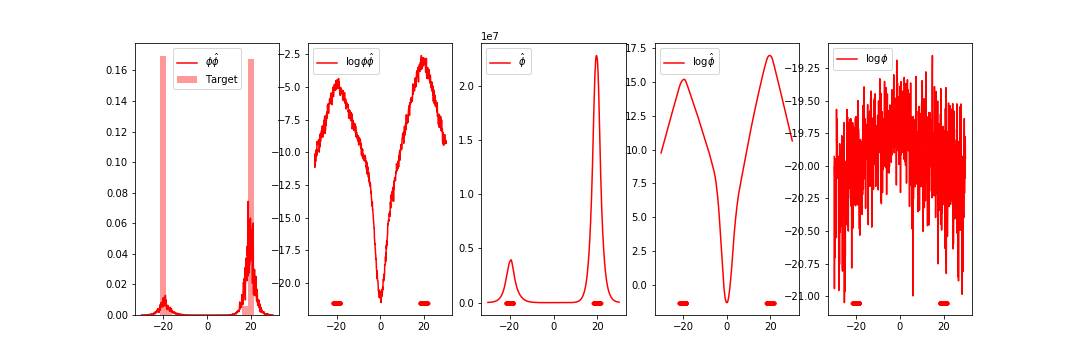
\includegraphics[scale=0.4,trim={2.3cm 0 1.5cm 1.5cm}, clip]{images/Pavon/Backward_bimodal_test_working.png} 
    \caption{Schrödinger Bridge results using the method by \cite{pavon2018data} on unimodal to bimodal Gaussian 1D data. }
    \label{fig:pavon_bimodal}
\end{figure}
\subsubsection{Delta Collapse}
In this section we explore how the method in \cite{pavon2018data} fails for small values of $\gamma$. In this case we use the different means, same variance dataset and set $\gamma=1$. We observed similar behaviour up to $\gamma=10$ and it was not until $\gamma=100$ that results became stable. In order to save time and avoid having to tweak $\gamma$ per experiment we choose an overly conservative value of $\gamma=1000$ which we used for all experiments in this section.

As shown in Figure \ref{fig:small_delta_collapse}, the learned marginal distributions have effectively collapsed into a Dirac delta function.  We believe this happens due to the transition probability not being able to hit points in the support of $\pi_0$ when mapping from $\pi_1$ (and vice-versa). The empirical proof backing this is the fact that this only happens for low values of $\gamma$ and that standardising the data or considering toy examples whose modes lie in the unit cube fixes this issue. We note that in \cite{pavon2018data} they use a value of $\gamma=2$ and furthermore the only 2 examples they have are distributions centered very closely to $0$, all with means $<3$, which is where we observe the cutoff to happen empirically. 
\subsection{Multimodal Experiments}
\begin{figure}[t]
    \centering
    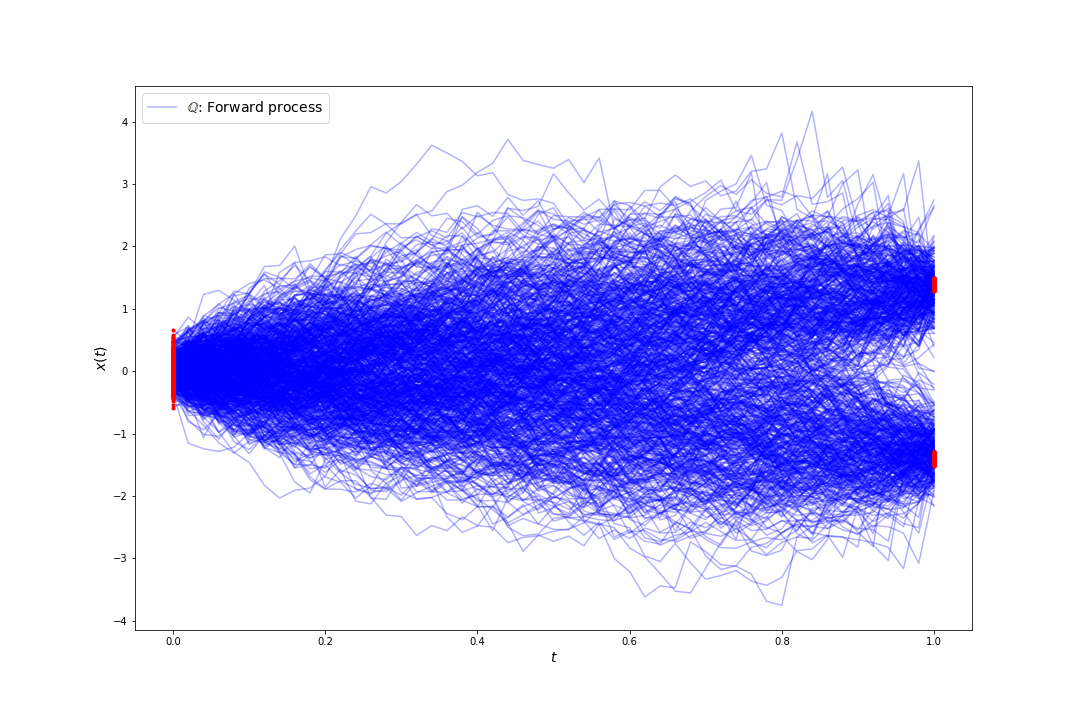
\includegraphics[scale=0.45,trim={2.3cm 1cm 2.5cm 0}, clip]{images/Pavon/pavon_trajectories_bimodal.png} 
    \caption{Extracted drift from optimal potentials. Marginals highlighted in red for visibility. }
    \label{fig:pavon_bimodal_drift}
\end{figure}
Unfortunately, we were unable to obtain sensible results for trimodal data with distinct modes, thus we focused solely on bimodal data where we managed to get this method working.
\begin{align*}
     \color{blue}{\pi_0(x)} &\color{blue}{= \calN(x; 0,  1)} \\
    \color{red}{\pi_1(y)} &\color{red}{= \frac{1}{2}\calN(y; 20, 0.5 ^2) + \frac{1}{2}\calN(y; -20, 0.5 ^2)}. 
\end{align*}

As shown in Figure \ref{fig:pavon_bimodal}, the method correctly identifies the modes and in the case of $\color{blue}{\pi_1}$ it correctly identifies the variance. However, for $\color{red}{\pi_0}$ we can see that the method fits some slightly broader variances than that of the target. 
\subsection{Extracting the Optimal Drift}

Using Proposition 3.3 of \cite{pavon1991free}, we extract the optimal control signal/drift $\rvb_t^+$ from the potentials fitted in Figure \ref{fig:pavon_bimodal} by \cite{pavon2018data}'s method using: 
\begin{align*} 
    \rvb_t^{+} = \gamma \nabla \ln \phi^*_t(\vx(t)).
\end{align*}
\begin{figure}
    \centering
    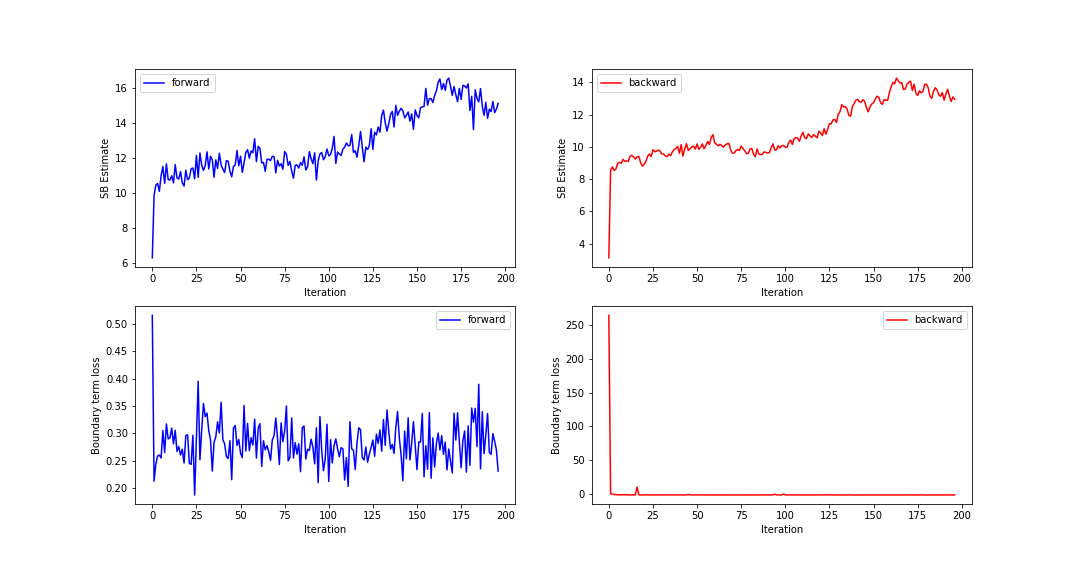
\includegraphics[scale=0.4,trim={2.3cm 1cm 2.5cm 0}, clip]{images/GP/SB_gp_bigvar_epochs_samp_200.png}
    \caption{Loss per epoch for fitted unimodal Schrödinger (SB) using the DDE method.}
    \label{fig:epochsbigvargp}
\end{figure}
We then generate trajectories using the EM method in order to visualise samples from the fitted path measure. Results can be seen in Figure \ref{fig:pavon_bimodal_drift}. Whilst the trajectories successfully split and manage to match the modes, they do not match the variances of the fitted potentials from Figure \ref{fig:pavon_bimodal}. This suggests that although the method from \cite{pavon2018data} may seem to solve the static bridge and provide some reasonable approximation for the potentials in the Schrödinger system, we are not able to recover a good estimate of the drift from these fitted potentials. This might be due to the inaccuracies arising from the importance sampling used in the method generating an overall poor estimate of the logarithmic derivative. We do note that the method by \cite{pavon2018data} does seem to provide reasonable estimates to the solution of the FPK equation and thus one can still interpolate the fitted distribution at different times.

\begin{figure}[t]
    \centering
    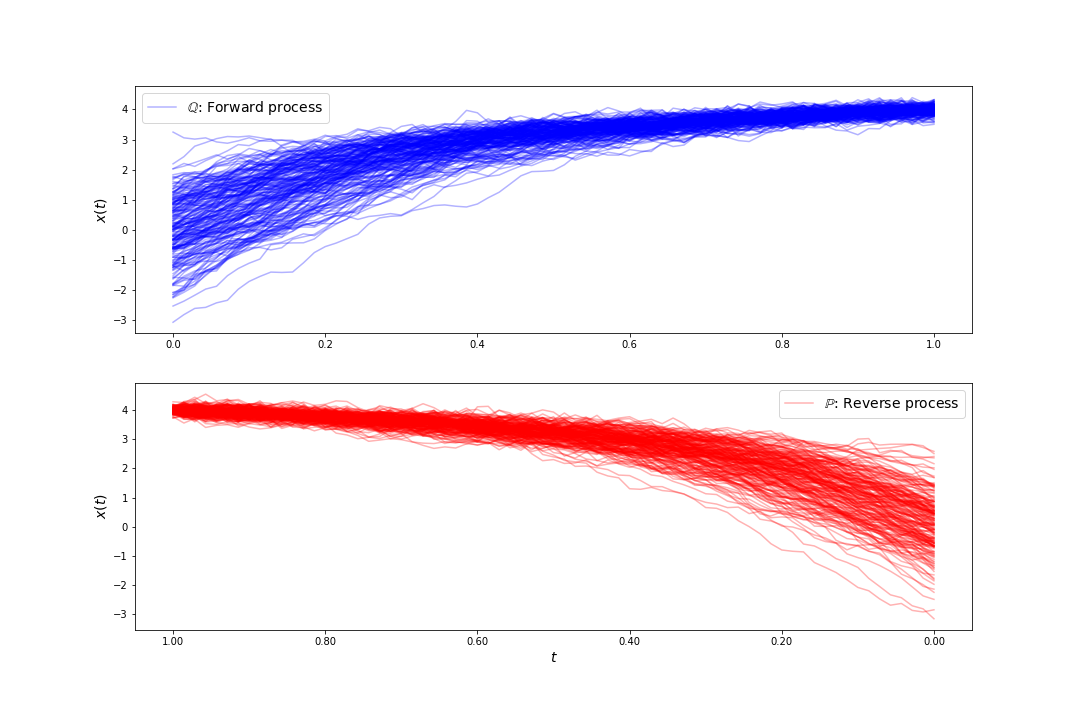
\includegraphics[scale=0.4,trim={2.3cm 1cm 2.5cm 0}, clip]{images/GP/gp_bigvar_trajectories.png}
    \caption{ Fitted SB trajectories using the DDE approach on unimodal to unimodal 1D data.  }
    \label{fig:bigvar200trajectroies}
\end{figure}
\section{Our Approach - Direct Drift Estimation (DDE)}

We found this approach to be much less brittle than the method by \cite{pavon2018data} when it came to distributions whose modes were far from the origin. However, it still suffers the problem that it cannot fit distributions whose support are too far from each other. We were empirically able to fit distributions whose means exceeded $4$ with a value of $\gamma=1$. All experiments in this section were performed with $\gamma=1$ and in some cases we adapted the examples from previous sections to have smaller means in order to accommodate for the issue regarding relative support of the distributions that we mentioned earlier. An important detail is that we did not optimise the hyperparameters of the fitted GP, this was mostly due to time constraints. Due to the typical memory constraints in Gaussian processes, we use 200 datapoints in each toy dataset and 70 time steps for the EM method.

\subsection{1D Toy Experiments }
\subsubsection{Unimodal Experiments}
Given the success of this method in more complex tasks, we omit the simple experiment of mapping in between different mean but shared variance Gaussian distributions.
\begin{figure}
    \centering
    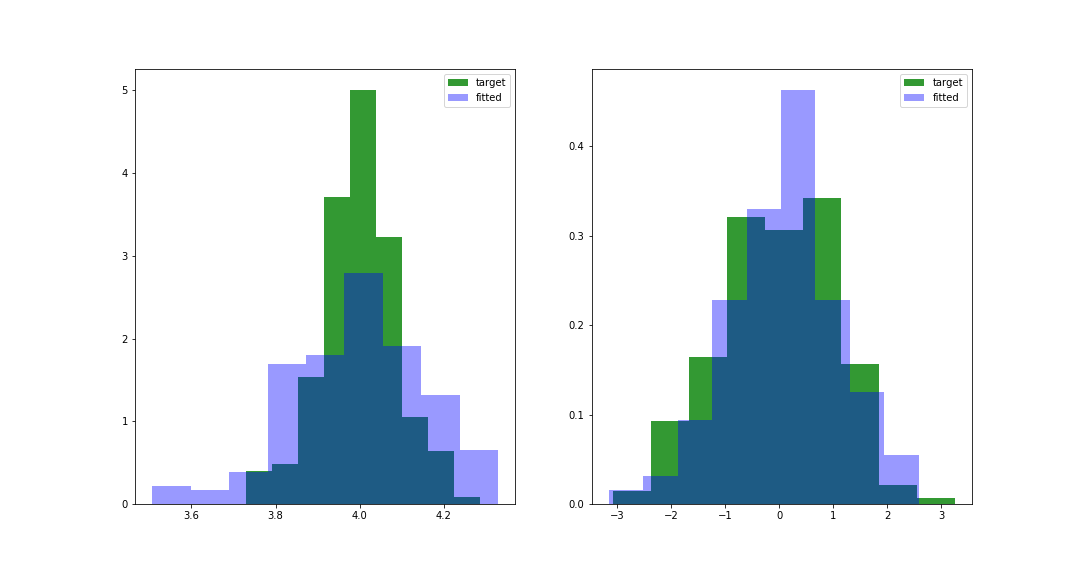
\includegraphics[scale=0.3,trim={2.3cm 1cm 2.5cm 0}, clip]{images/GP/gp_bigvar_boundaires.png}
    \caption{ Fitted SB marginals using the DDE approach on unimodal to unimodal 1D data.  }
    \label{fig:bigvar200boundaries}
\end{figure}
\\
\textbf{Different Means and Variances}\\
We generate this dataset following:
\begin{align*}
\color{blue}{\pi_0(x)} &\color{blue}{= \calN(x; 0,  1)} \\
    \color{red}{\pi_1(y)} &\color{red}{= \calN(y; 4, 0.1^2)}.
\end{align*}
We can observe from Figure \ref{fig:bigvar200trajectroies} that the trajectories match the correct evolution of the means and the variances. Inspecting Figure \ref{fig:bigvar200boundaries}, we can observe a minor struggle in matching the $0.1$ variance for which our approach seems to estimate a slightly higher variance. Overall we can observe a good fit.

\subsubsection{Multimodal Experiments}

We experiment with mapping in between unimodal and multimodal distributions. We empirically find that this is the only method that can robustly cope with more than 2 modes.

\textbf{Unimodal to Bimodal}\\
We follow the generative following generative process for generating the toy data:
\begin{align*}
     \color{blue}{\pi_0(x)} &\color{blue}{= \calN(x; 0,  1)} \\
    \color{red}{\pi_1(y)} &\color{red}{= \frac{1}{2}\calN(y; 1.8, 0.6 ^2)}\color{red}{ + \frac{1}{2}\calN(y; -1.9, 0.6 ^2) }.
\end{align*}
\begin{figure}
    \centering
    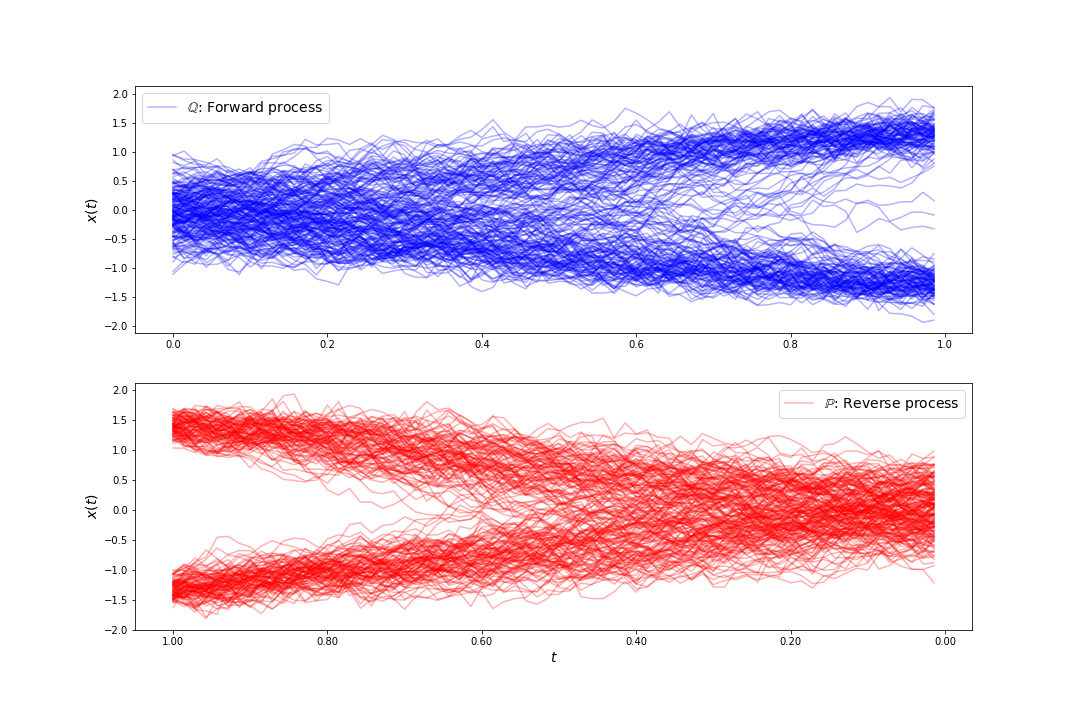
\includegraphics[scale=0.4,trim={2.3cm 1cm 2.5cm 0}, clip]{images/GP/gp_final_bimodal_trajectories.png}
    \caption{ Fitted SB trajectories using the DDE method on the unimodal to bimodal 1D dataset.  }
    \label{fig:bimodfinal200trajectories}
\end{figure}
\begin{figure}
    \centering
    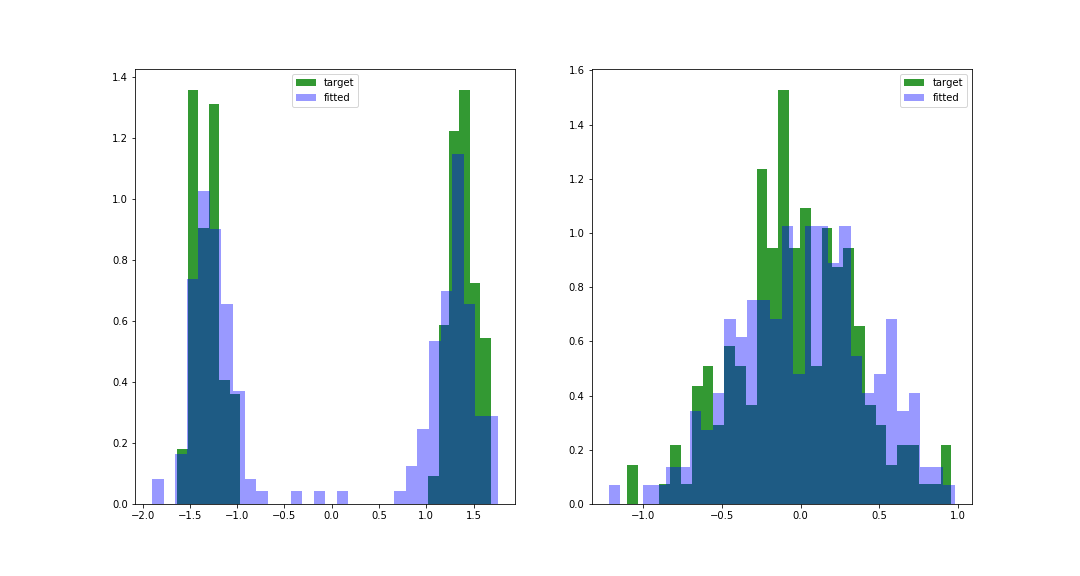
\includegraphics[scale=0.3,trim={4cm 1cm 2.5cm 0}, clip]{images/GP/gp_2_mode_final_boundaires.png}
    \caption{ Fitted SB marginals using the DDE method on the unimodal to bimodal 1D dataset.  }
    \label{fig:bimodfinal200boundaries}
\end{figure}
Results can be found in Figures \ref{fig:bimodfinal200boundaries} and \ref{fig:bimodfinal200trajectories}. We observe mostly a good fit for the unimodal boundary and for the bimodal boundary with the exception of $3$ outliers that were transported to an area that should have close to $0$ probability mass.  
We found that these outliers occurred outside of the Schrödinger bridge context and rather due to the method by \cite{ruttor2013approximate} (used for fitting the drift of SDEs) struggling in matching low variances at the boundaries. It is possible that optimising the GPs hyperparameters may also improve on this. 

\textbf{Unimodal to Trimodal}\\
\begin{figure}[t]
    \centering
    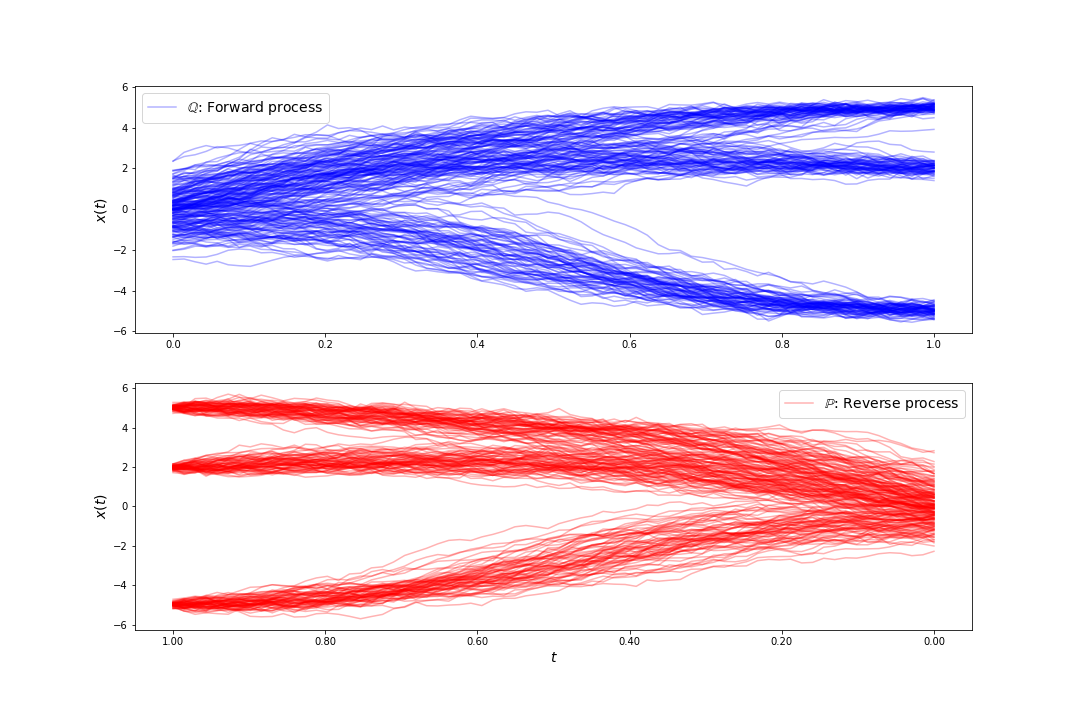
\includegraphics[scale=0.4,trim={2.3cm 1cm 2.5cm 0}, clip]{images/GP/gp_3_mode_200_trimodal_boundaires_trajectories.png}
    \caption{ Fitted SB trajectories for unimodal to trimodal data using DDE, successfully fitting three modes.  }
    \label{fig:3mode1d200trajectroies}
\end{figure}
We generate the 1D toy dataset following the following distribution:
\begin{align*}
     \color{blue}{\pi_0(x)} &\color{blue}{= \calN(x; 0,  1)} \\
    \color{red}{\pi_1(y)} \color{red}{= \frac{1}{3}\calN(y; 5, 0.5 ^2)}&\color{red}{ + \frac{1}{3}\calN(y; 2, 0.5 ^2) + \frac{1}{3}\calN(y; -5, 0.5 ^2)}.
\end{align*}
\begin{figure}
    \centering
    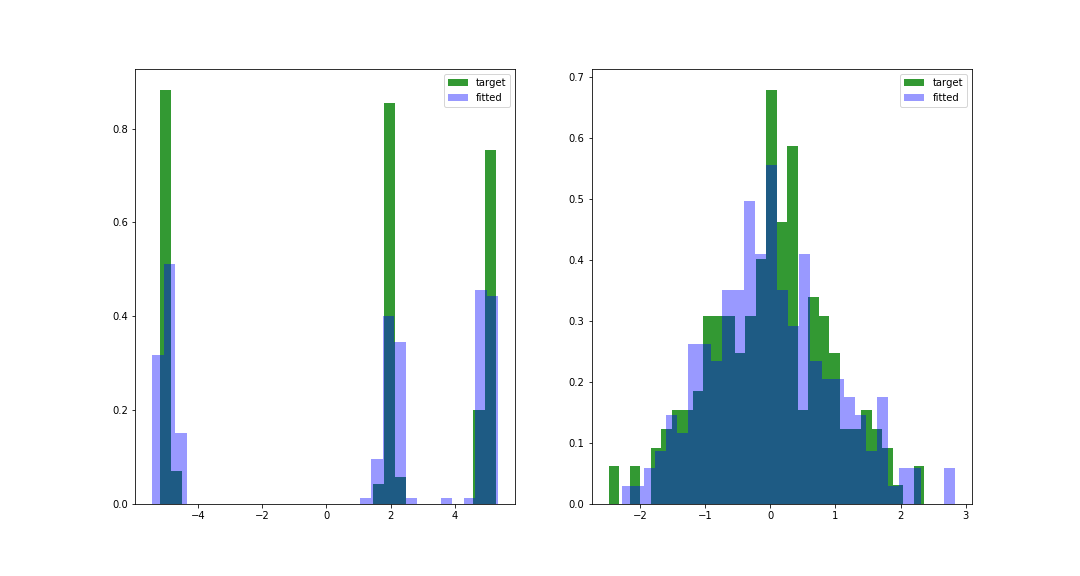
\includegraphics[scale=0.3,trim={2.3cm 1cm 2.5cm 0}, clip]{images/GP/gp_3_mode_200_boundaires.png}
    \caption{ Fitted SB trajectories for unimodal to trimodal data using DDE.  }
    \label{fig:3mode1d200boundaries}
\end{figure}
We can observe from Figures \ref{fig:3mode1d200trajectroies}, \ref{fig:3mode1d200boundaries} that the boundaries distributions are matched  nicely both in variance and mean. Furthermore, the trajectories look sound: they have some reminiscence of Brownian motion, follow nice simple paths, and look dual to each other. We also observe that for the two modes that are close to each other there are two outliers in low probability areas.
\subsection{2D Toy Experiments}

Given the success of the DDE method in going beyond splitting two modes, we decided to experiment further and go into 2-dimensions. Due to time constraints we chose not to carry out 2-dimensional experiments for the method in \cite{pavon2018data}, furthermore we were unable to get their method to split beyond 2 modes. 

\subsubsection{Trimodal Experiment}
In this section we consider the 2D extension of the trimodal experiment.   We use the following distributions to generate our toy examples:

\begin{figure}[H]
\begin{adjustbox}{width=\columnwidth}
\parbox{\linewidth}{
\begin{align*}
    \color{blue}{\pi_0(\vx)} &\color{blue}{= \calN\Bigg(\vx; -{0.1\choose0.1},  0.19^2\, \mathbb{I}_2 \Bigg)} \\
    \color{red}{\pi_1(\vy)} \color{red}{= \frac{1}{3}\calN\Bigg(\!\vy; -{3.3\choose0.1}, 0.11^2\mathbb{I}_2\!\Bigg)}&\color{red}{ + \frac{1}{3}\calN\Bigg(\!\vy; {3.5\choose3.5}, 0.11 ^2\mathbb{I}_2\!\Bigg)}\!+\color{red}{ \frac{1}{3}\calN\Bigg(\!\vy; {0.7\choose0.7}, 0.11 ^2\mathbb{I}_2\!\Bigg)}
\end{align*}
}
\end{adjustbox}
\end{figure}
% \end{adjustbox}
\begin{figure}
    \centering
    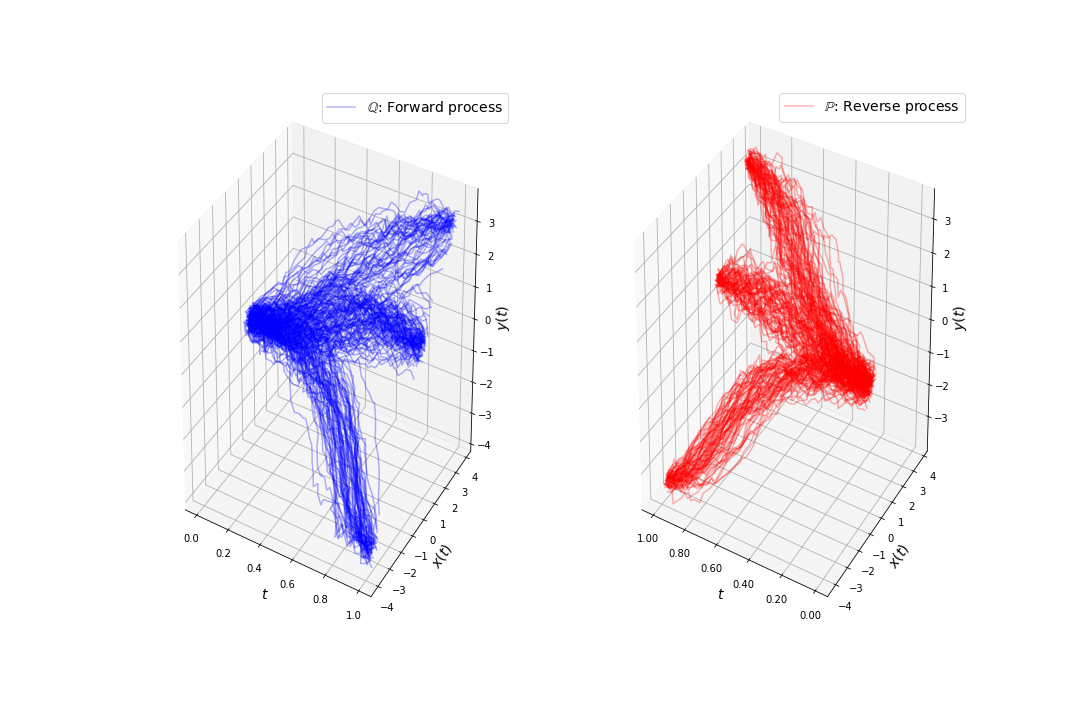
\includegraphics[scale=0.4,trim={5.3cm 1cm 2.5cm 0}, clip]{images/GP/2d_3mode_GP_means_3.3_3.6_0.7_std_0.1_200.png}
    \caption{ Fitted SB trajectories using the DDE method for unimodal to trimodal data.  }
    \label{fig:3mode2d200trajectroies2d}
\end{figure}
From Figure \ref{fig:3mode2d200trajectroies2d}  we can see how the trajectories successfully split and merge into 3 modes.
\begin{figure}
    \centering
    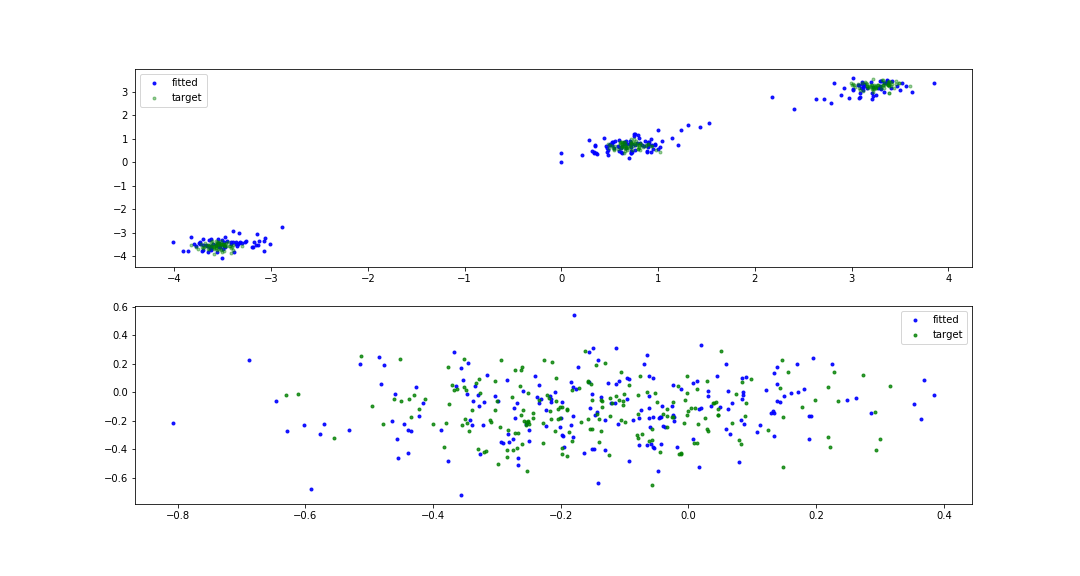
\includegraphics[scale=0.4,trim={2.3cm 1cm 2.5cm 0}, clip]{images/GP/2d_3mode_GP_means_3.3_3.6_0.7_std_0.1_scatter_200_.png}
    \caption{ Fitted SB marginals using the DDE method for unimodal to trimodal data.}
    \label{fig:3mode2d200}
\end{figure}
\begin{figure}
    \centering
    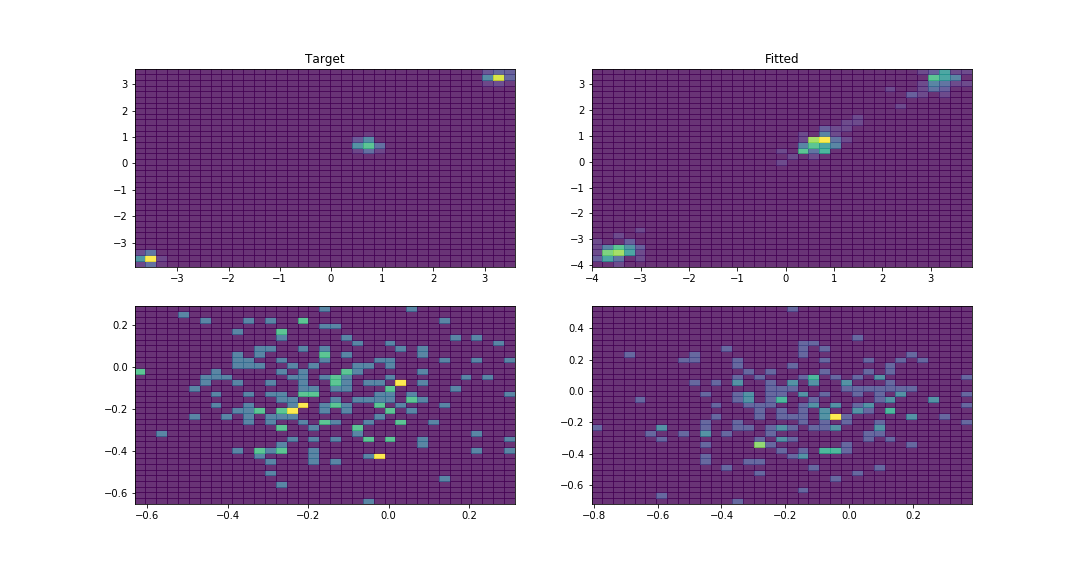
\includegraphics[scale=0.4,trim={2.3cm 1cm 2.5cm 0}, clip]{images/GP/2d_3mode_GP_means_3.3_3.6_0.7_std_0.1_hist_200.png}
    \caption{ 2D histograms for the fitted SB marginals using the DDE method for unimodal to trimodal data.  On the left we show the true empirical distribution and on the right we show the empirical distribution learned by our Schrödinger bridge mapping.}
    \label{fig:3mode2d200hist}
\end{figure}
In Figure \ref{fig:3mode2d200} we observe that the marginal constraints are enforced to a reasonable amount, matching means quite well, yet struggling partly with the variance of the low variance boundaries.
% In general, we found that in two dimensions this method struggled in matching small variances. This issue occurs when fitting the drift of SDEs in general using the method by \cite{ruttor2013approximate}.
\subsubsection{Circles Dataset}

\begin{figure}
    \centering
    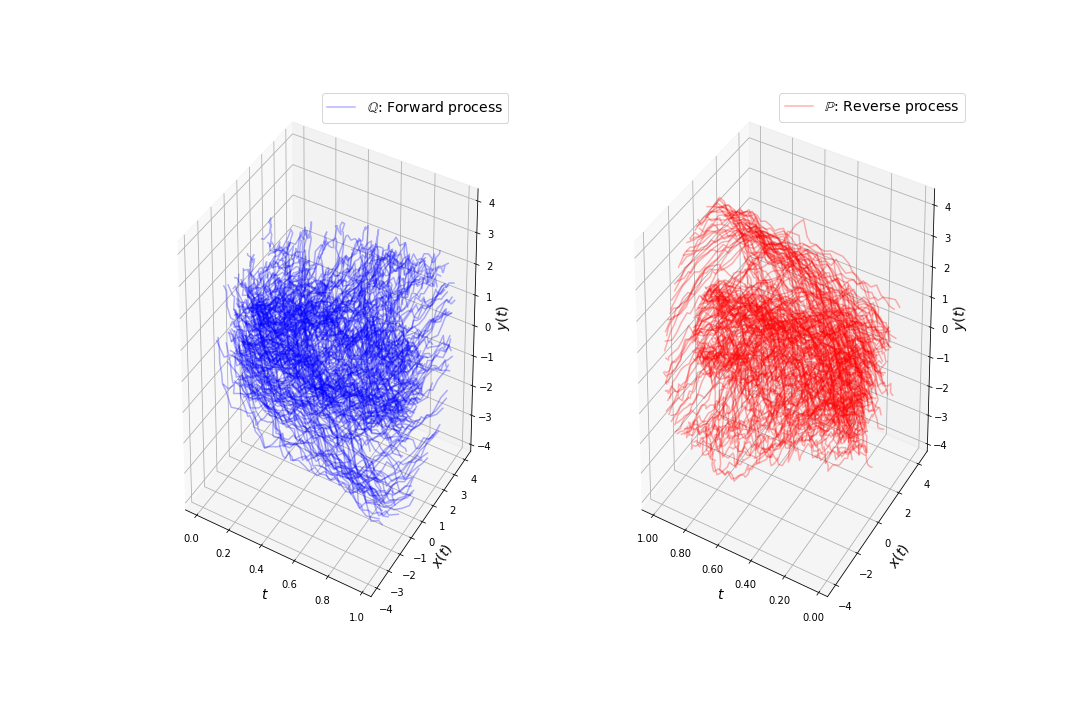
\includegraphics[scale=0.4,trim={5.3cm 2cm 2.5cm 0}, clip]{images/GP/gp_circles_trajectories_200_big.png}
    \caption{ Fitted SB trajectories using the DDE method for unimodal to circles data.  We can observe the nice and clear concentric circles trajectories arising in the learned bridge. }
    \label{fig:circ2d200trajectroies2d}
\end{figure}
\begin{figure}
    \centering
    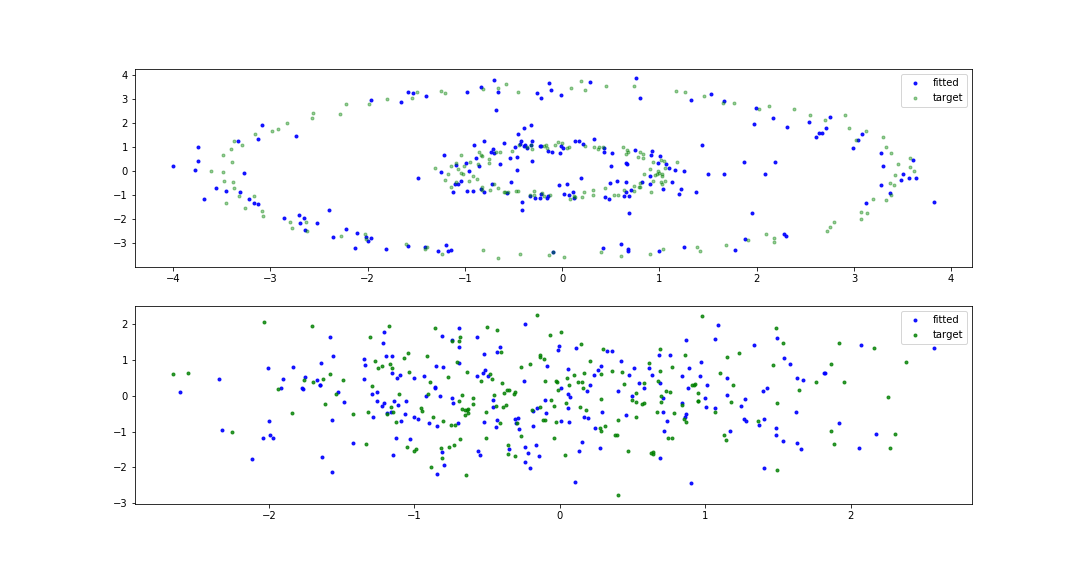
\includegraphics[scale=0.4,trim={2.3cm 1cm 3.5cm 0}, clip]{images/GP/gp_circles_scatter_200_big_.png}
    \caption{ Fitted SB Boundary distributions using the DDE method on unimodal to circles data.}
    \label{fig:circ2d200scatter2d}
\end{figure}
\begin{figure}
    \centering
    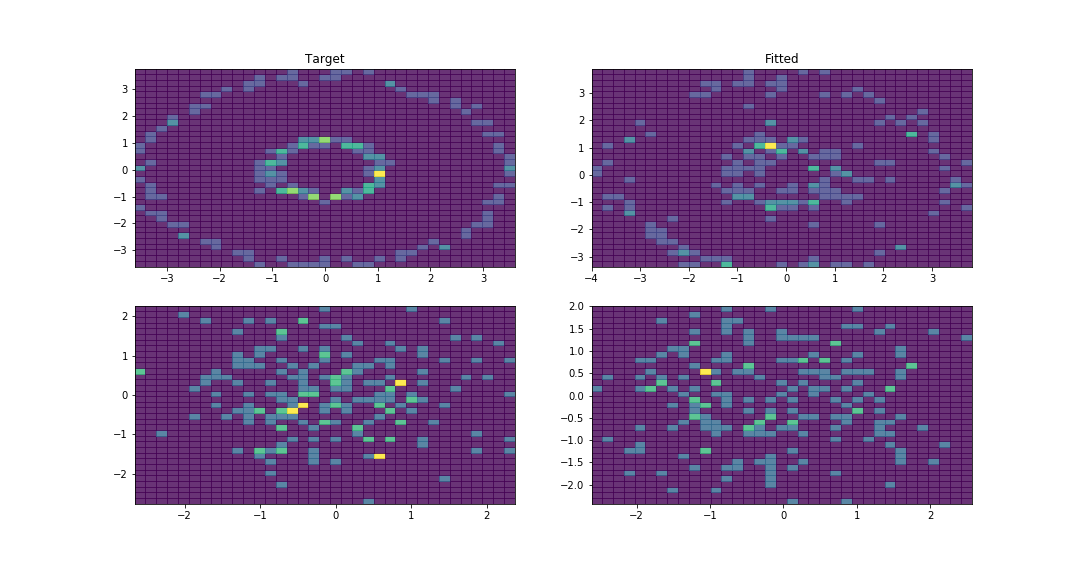
\includegraphics[scale=0.4,trim={2.3cm 1cm 2.5cm 0}, clip]{images/GP/gp_circles_hist_200_big.png}
    \caption{ 2D histograms for the fitted SB marginals using the DDE method for unimodal to circles data.}
    \label{fig:circ2d20hist2d}
\end{figure}
We  used the circles dataset \citep{pedregosa2011scikit} which consists of two concentric circles. In this task we consider mapping from a standardised unimodal Gaussian to the Circles data.
\begin{align*}
     \color{blue}{\pi_0(\vx)} &\color{blue}{= \calN(\vx; \vzero,  \mathbb{I}_2)} \\
    \color{red}{\hat{\pi}_1(\vy)} &\color{red}{= \text{GenerateCircles(factor=0.3, radius=3.5, noise=0.03)}}.
\end{align*}
The radius and factor (distance between circles) were picked so the data was still within a close proximity to the origin, whilst making the circles distinct.

We can see from Figure \ref{fig:circ2d200trajectroies2d} that some very structured inner circle-like trajectories are formed going forward and backward with a dual like pattern. Furthermore, from Figures \ref{fig:circ2d200scatter2d}, \ref{fig:circ2d20hist2d} we can observe a good fit in terms of structure, but the fits of our method are slightly more dispersed, with higher variance. We noticed this can be improved by using more training data and tweaking the GP hyper-parameters. Further experiments should be carried out to diagnose and solve this issue. 


\subsubsection{Moons Dataset}
We use the moons dataset from \cite{pedregosa2011scikit}, generated by the following procedure:
\begin{align*}
     \color{blue}{\pi_0(\vx)} &\color{blue}{= \calN(\vx; \vzero,  \mathbb{I}_2)} \\
    \color{red}{\hat{\pi}_1(\vy)} &\color{red}{= \text{GenerateMoons(scale\_x=1.8, scale\_y=3.8, noise=0.03)}}.
\end{align*}
Similar to the circles dataset, the scales were picked to give a nice visual scale and a clear separation between the moons, making the task as simple as possible given that we were still in an exploratory stage.

\begin{figure}
    \centering
    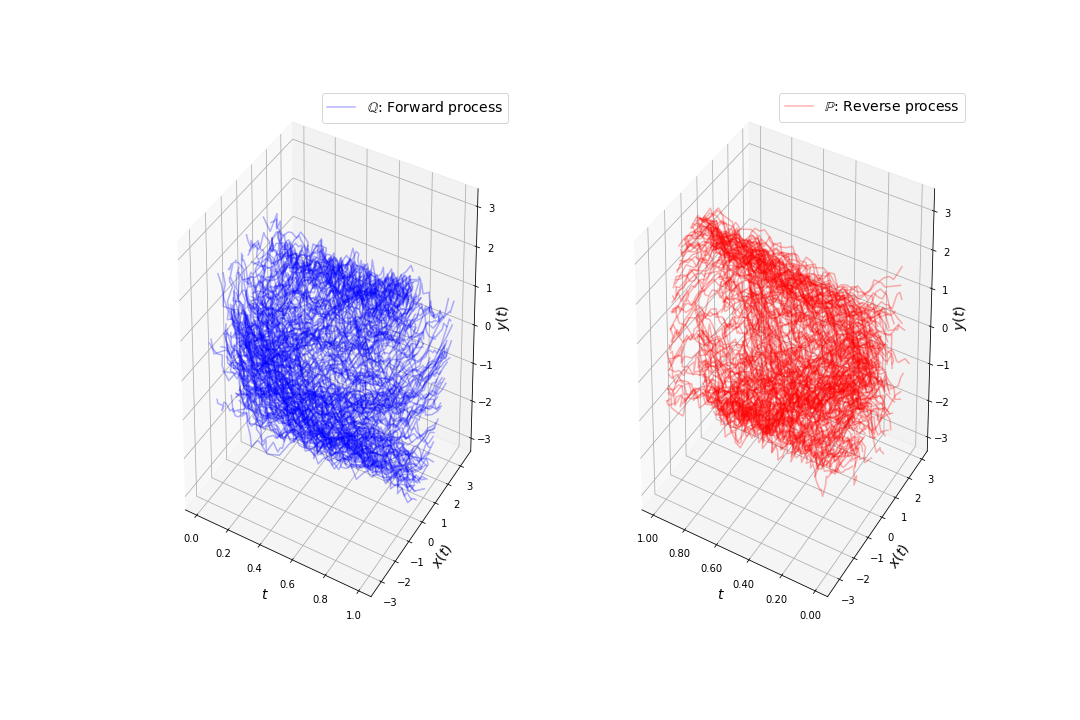
\includegraphics[scale=0.4,trim={5.3cm 1cm 2.5cm 0}, clip]{images/GP/moons_2d_gp_trajectories_short_200.png}
    \caption{ Fitted SB trajectories using the DDE method for unimodal to moons data.  }
    \label{fig:moon2d200trajectroies2d}
\end{figure}
\begin{figure}
    \centering
    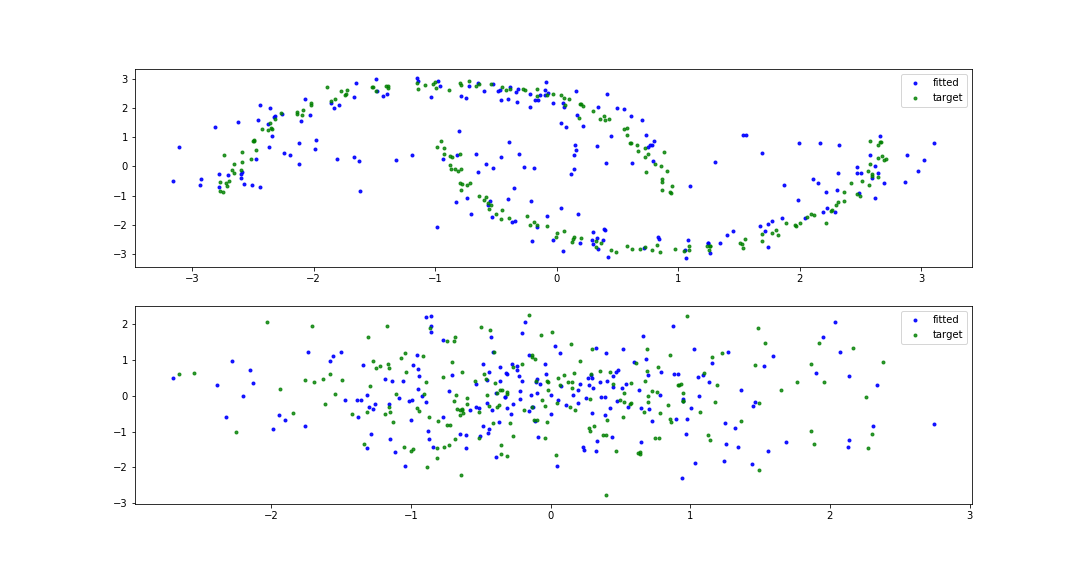
\includegraphics[scale=0.4,trim={2.3cm 1cm 2.5cm 0}, clip]{images/GP/gp_moons_scatter_200_big_.png}
    \caption{ Fitted SB Boundary distributions using the DDE method for unimodal to moons data.}
    \label{fig:moon2d200scatter2d}
\end{figure}
\begin{figure}
    \centering
    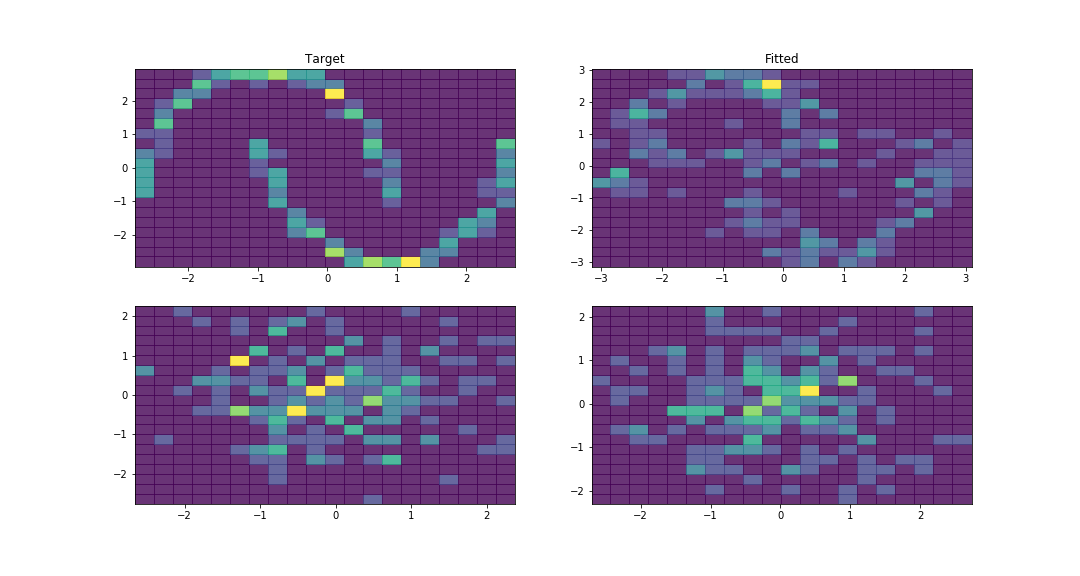
\includegraphics[scale=0.4,trim={2.3cm 1cm 2.5cm 0}, clip]{images/GP/moons_2d_gp_hist_short_200.png}
    \caption{2D histograms for the fitted SB marginals using the DDE method for unimodal to moons data.}
    \label{fig:moon2d20hist2d}
\end{figure}

We use the moons dataset from \cite{pedregosa2011scikit}, generated by the following procedure:
\begin{align*}
     \color{blue}{\pi_0(\vx)} &\color{blue}{= \calN(\vx; \vzero,  \mathbb{I}_2)} \\
    \color{red}{\hat{\pi}_1(\vy)} &\color{red}{= \text{GenerateMoons(scale\_x=1.8, scale\_y=3.8, noise=0.03)}}.
\end{align*}
Similar to the circles dataset, the scales were picked to give a nice visual scale and a clear separation between the moons. This makes the task as simple as possible, given that we were still in an exploratory stage.

\begin{figure}
    \centering
    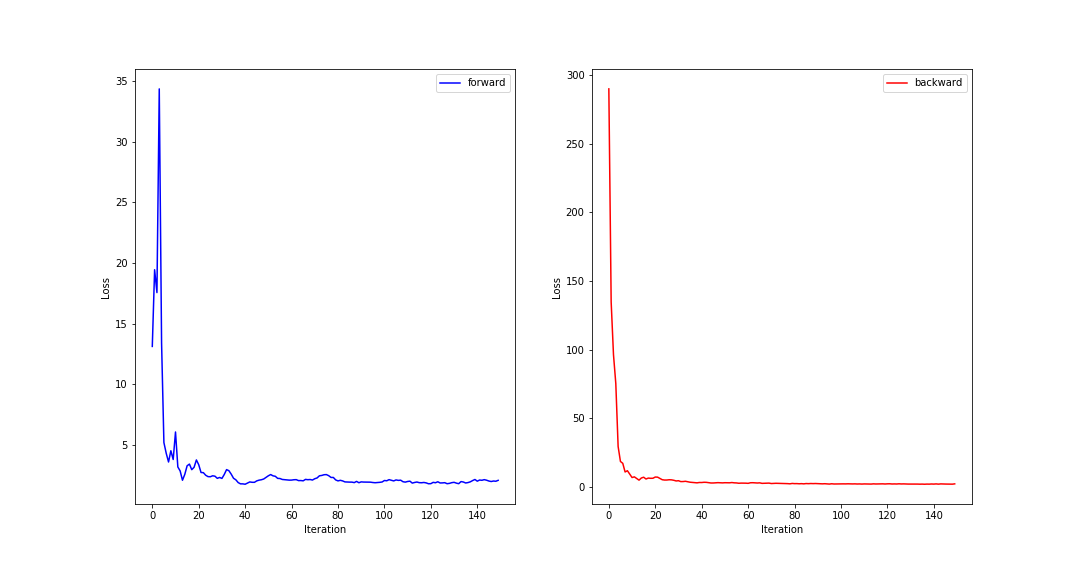
\includegraphics[scale=0.4,trim={2.3cm 1cm 2.5cm 0cm}, clip]{images/Control/big_var_loss.png}
    \caption{Loss per epoch for fitted unimodal SB using tanh activation, single layer and 200 hidden units for SC approach.}
    \label{fig:epochsbigvarnn}
\end{figure}
\begin{figure}[t]
    \centering
    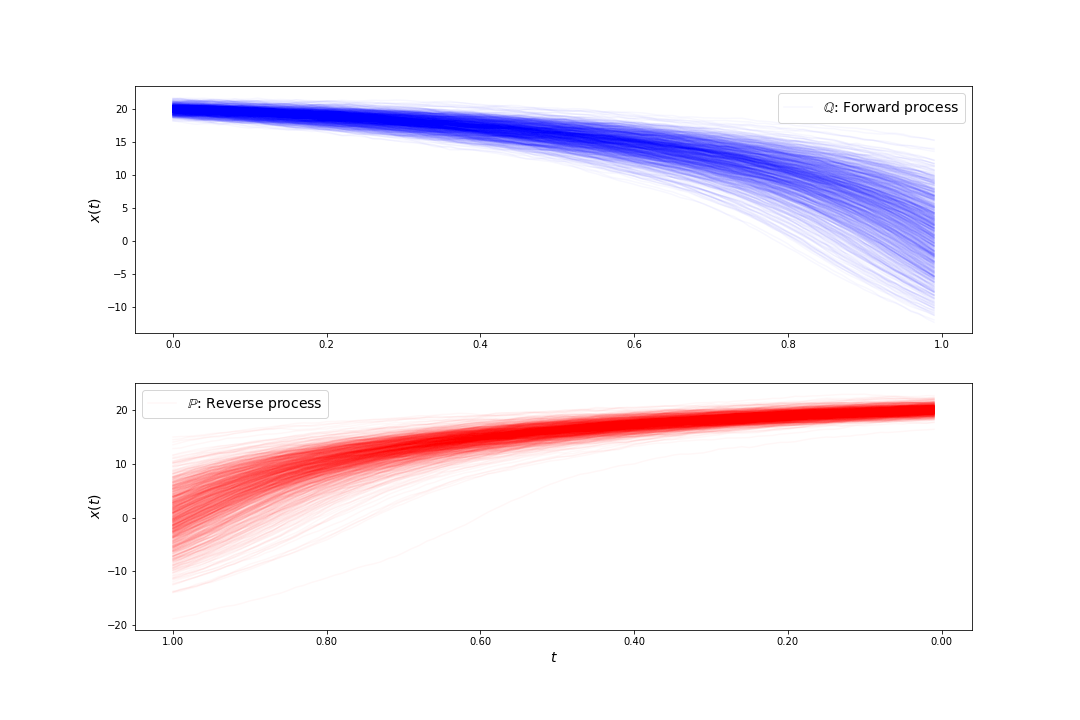
\includegraphics[scale=0.4,trim={2.3cm 1.9cm 2.5cm 2cm}, clip]{images/Control/big_var_marginals_best_tanh_trajectories.png}
    \caption{ Fitted SB trajectories using the SC method with tanh activations, single layer and 200 hidden units, fitted on the unimodal dataset. Note that the trajectories seem much smoother than the ones induced by the direct drift approach. This is mostly a visual effect due to the scale of the y axis being much higher. In other words you will see less noise if you zoom out.}
    \label{fig:trajectoriesbigvarnn}
\end{figure}
\section{Stochastic Control (SC)  Approach}


Throughout this section we employ neural networks \citep{lecun2015deep} to parametrise the drifts in Equation \ref{eq:drift_param} and experiment with 3 different types of activations: Tanh, Hard Tanh, ReLu.  We varied layer widths and depths in order to obtain good results, without careful regard for overfitting, since, as mentioned, we are merely exploring the capacities and faults of the approaches. Across all experiments, we initialise the weights of the neural networks using Glorot initialisation \citep{glorot2010understanding} and we used the Adagrad optimiser \citep{duchi2011adaptive}. Due to the KNN based approach to computing cross entropy being unstable, we used the KDE based approach across all experiments. This method allowed using bigger datasets than the previous two methods, thus we used 900 datapoints in each toy dataset, 100 time steps for the EM method and a batch size of 900 (only one batch) for the optimiser. 

\subsection{Unimodal Experiments}
For the unimodal experiments we focus on mapping between normal distributions with different means and variances.
\subsubsection{Small to Big Variance}

Data was generated using:
\begin{align*}
\color{blue}{\pi_0(x)} &\color{blue}{= \calN(x; 0,  3)} \\
    \color{red}{\pi_1(y)} &\color{red}{= \calN(y; 6, 0.1^2)} 
\end{align*}
\begin{figure}
    \centering
    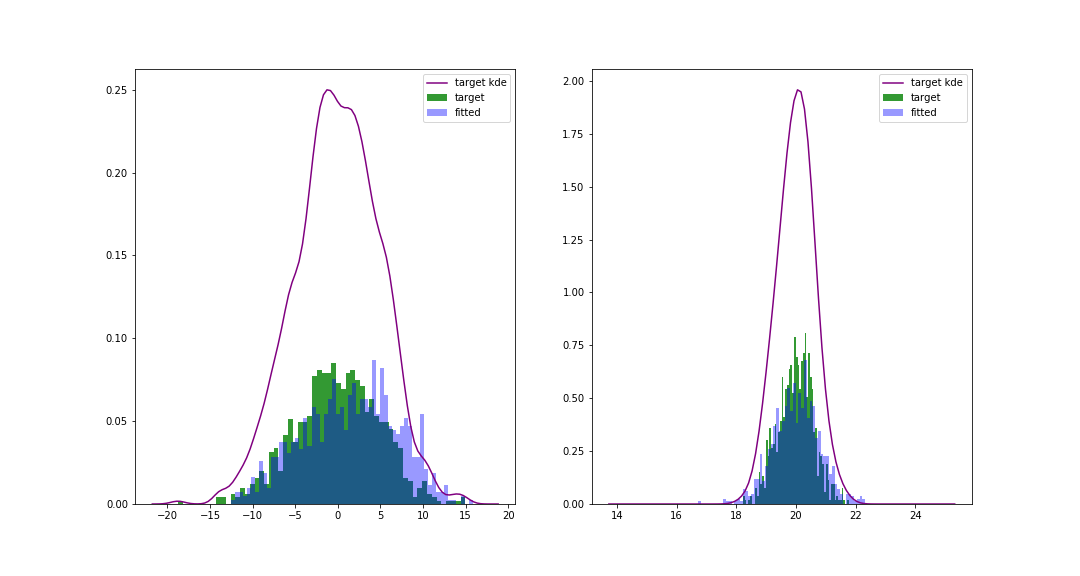
\includegraphics[scale=0.4,trim={2.3cm 2cm 2cm 2cm}, clip]{images/Control/big_variance_tanh_marginals.png}
    \caption{ Fitted SB  boundary distributions using the SC method with tanh activations, single layer and 200 hidden units. }
    \label{fig:boundsbigvarnn}
\end{figure}

For these particular experiments, we found very little differences among the trajectories learned by different activations. Results can be found in Figures \ref{fig:boundsbigvarnn} and \ref{fig:trajectoriesbigvarnn}, where we can see a good fit for the marginal with low variance, but a worse fit for the high variance distribution where the variance is matched but the mode is not.
\subsection{Multimodal Experiments}
In this section we followed the generative process:
\begin{align*}
     \color{blue}{\pi_0(x)} &\color{blue}{= \calN(x; 0,  1)} \\
    \color{red}{\pi_1(y)} &\color{red}{= \frac{1}{2}\calN(y; 20, 0.6 ^2)}\color{red}{ + \frac{1}{2}\calN(y; -20, 0.6 ^2) }.
\end{align*}
We parametrised the drifts with 3 hidden layers, each having 20 hidden units, with the exception of the final experiment and best performing model for which we used 2 hidden layers, each with 200 units. In general, we found that increasing the number of units and layers made the optimisation process more unstable and typically required reducing the initial step size for the optimiser. These experiments are used for investigating how the stochastic control based approach can handle mode collapse.
\subsubsection{ReLu}
\begin{figure}
    \centering
    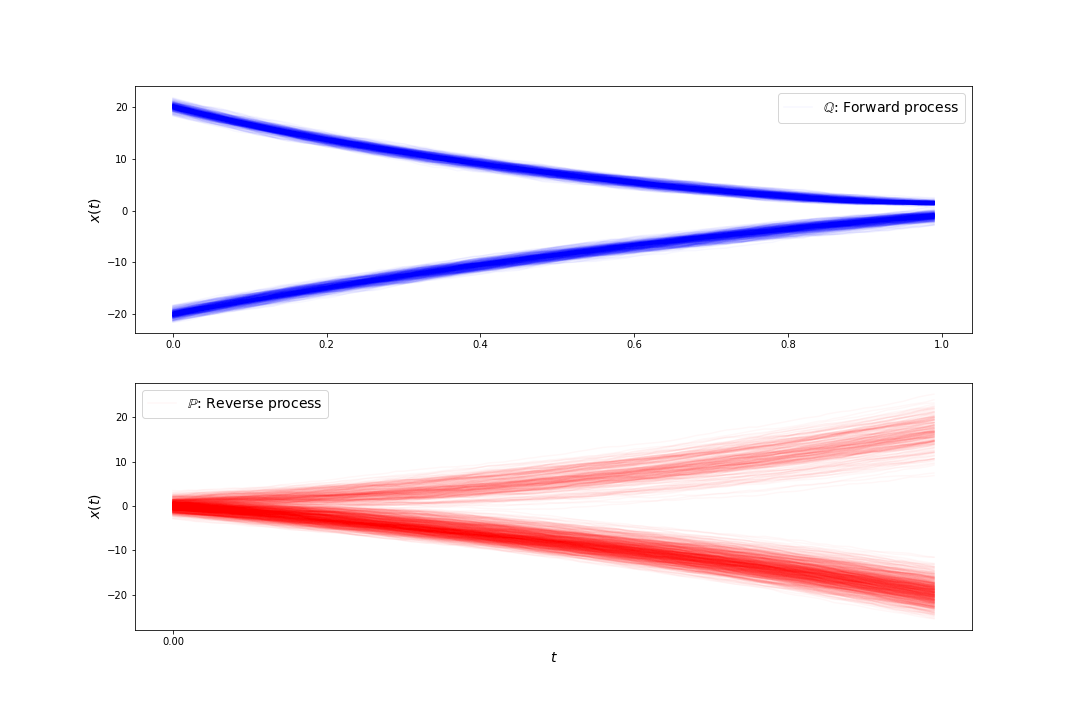
\includegraphics[scale=0.4,trim={2.3cm 1cm 2.5cm 0}, clip]{images/Control/bimod_final_relu_trajectories.png}
    \caption{ Fitted SB  trajectories using ReLu activation, 3 hidden layers of 20 hidden units each}
    \label{fig:trajectoriesbimodrelunn}
\end{figure}
\begin{figure}
    \centering
    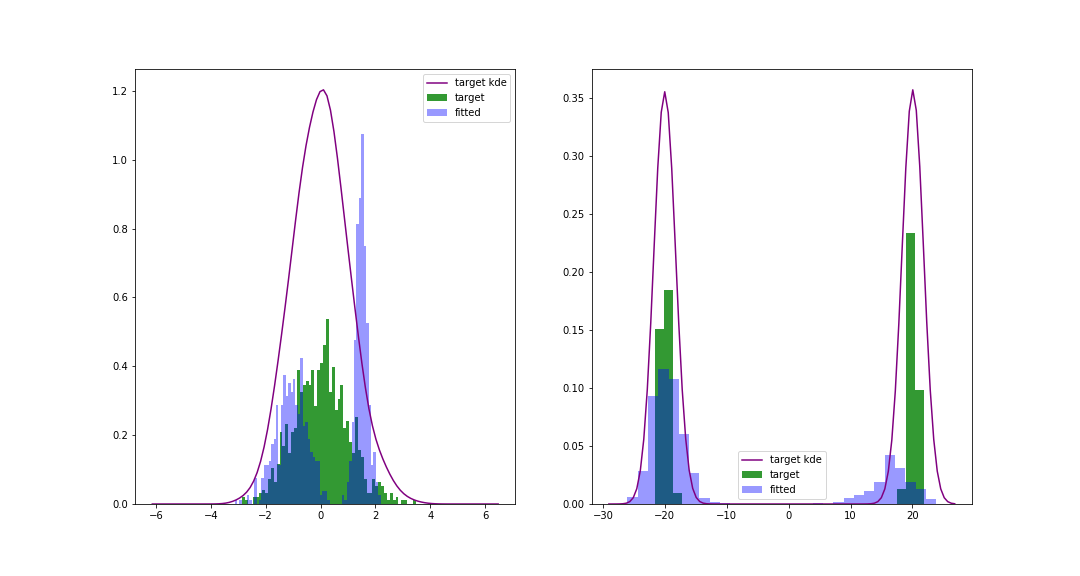
\includegraphics[scale=0.4,trim={2.3cm 1cm 2.5cm 0}, clip]{images/Control/bimod_final_relu_boundaires.png}
    \caption{ Fitted SB  boundary distributions using the SC method with ReLu activations, 3 hidden layers of 20 hidden units each.}
    \label{fig:boundsbimodrelunn}
\end{figure}
\begin{figure}
    \centering
    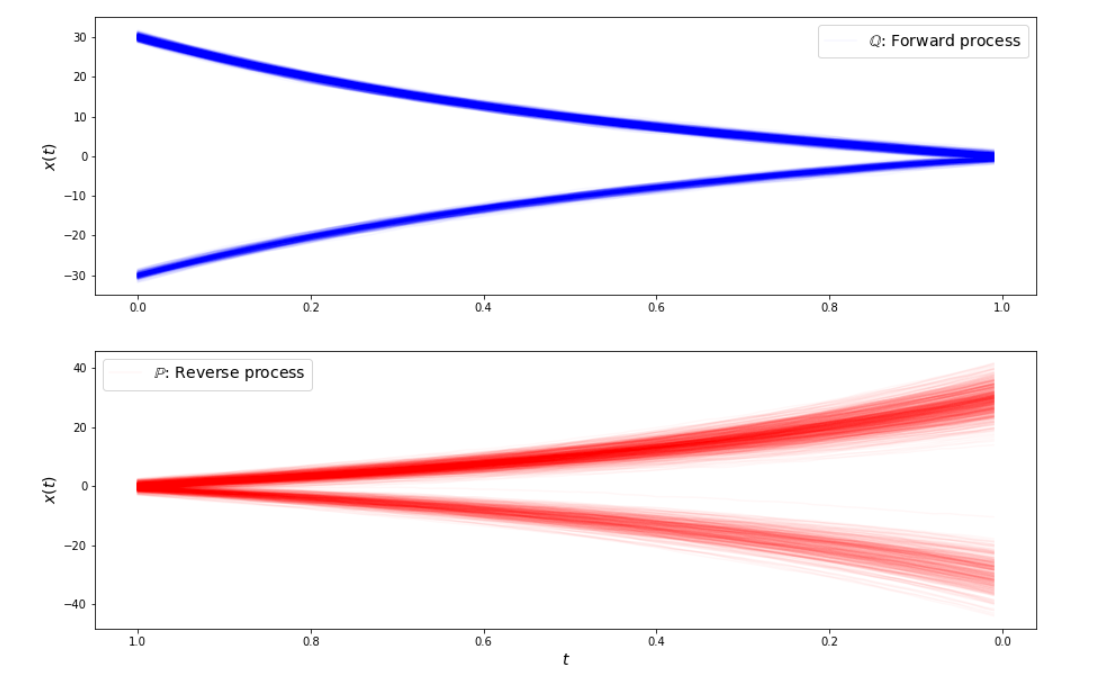
\includegraphics[scale=0.7,trim={0cm 0cm 0cm 0}, clip]{images/Control/almost_perfect_bimodal_relu.PNG}
    \caption{ Additional bimodal experiment - Fitted SB  trajectories using the SC method with ReLu activations, 3 hidden layers of 20 hidden units each.}
    \label{fig:trajectoriesbimodrelunn_}
\end{figure}

For these experiments, we use the rectified linear-unit (ReLu) \citep{glorot2011deep}. We show results of a further experiment with larger means to illustrate the shape of the trajectories induced by this activation. As shown in Figures \ref{fig:trajectoriesbimodrelunn} and \ref{fig:trajectoriesbimodrelunn_}, the learned trajectories are more curved (almost parabolic like) than the trajectories induced by tanh based activations. We also observe that whilst being on the right track to matching the means, it fails to match the variance of the bimodal marginals. One positive aspect is that the curves do have a dual like nature.

\subsubsection{Tanh}

Here we use the hyperbolic-tangent (Tanh) as the activation function. We also experimented with similar smooth activations and obtained similar results.
\begin{figure}
    \centering
    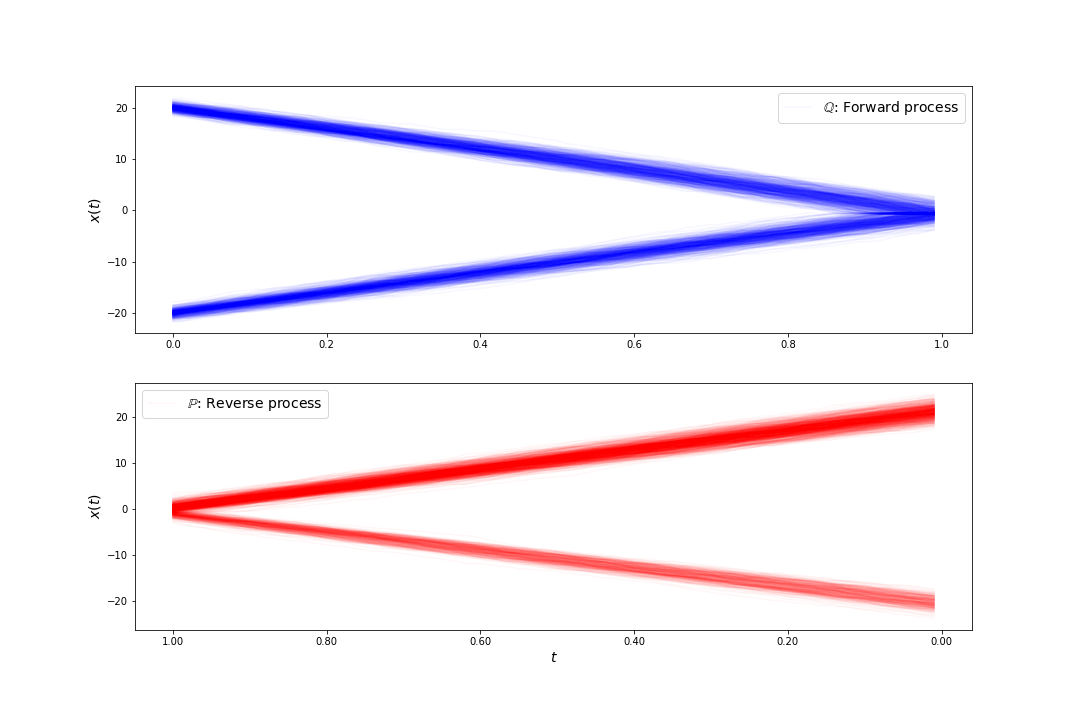
\includegraphics[scale=0.4,trim={2.3cm 1cm 2.5cm 0}, clip]{images/Control/bimodal_marginals_best_tanh_trajectories.png}
    \caption{ Fitted SB  trajectories using the SC method with tanh activations, 3 hidden layers of 20 hidden units each.}
    \label{fig:trajectoriesbimodtanhnn}
\end{figure}
\begin{figure}
    \centering
    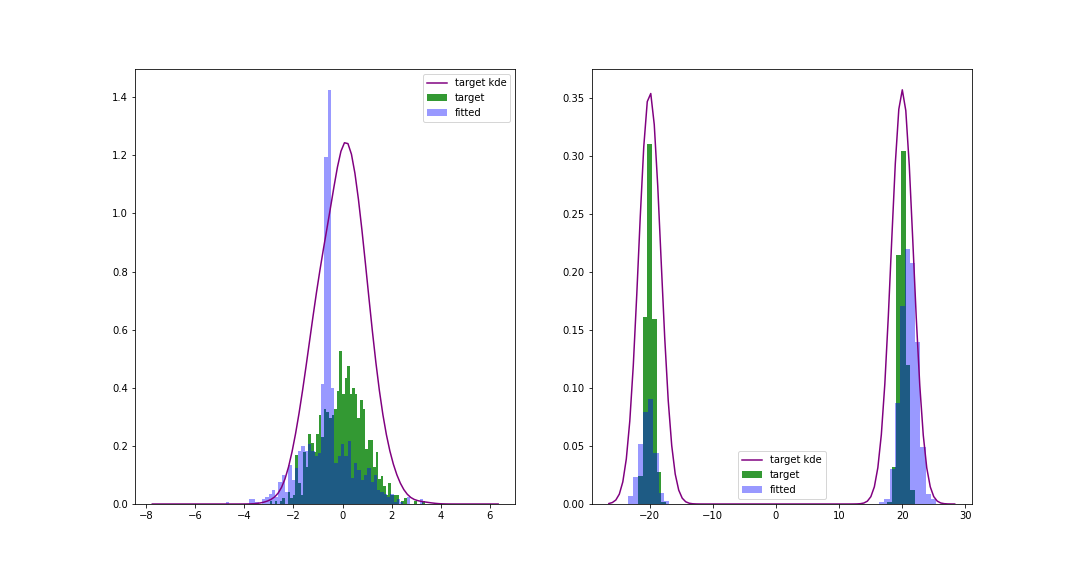
\includegraphics[scale=0.4,trim={2.3cm 1cm 2.5cm 0}, clip]{images/Control/bimodal_marginals_best_tanh.png}
    \caption{ Fitted SB  boundary distributions using the SC method with tanh activations, 3 hidden layers of 20 hidden units each.}
    \label{fig:boundsbimodtanhnn}
\end{figure}
We observe from Figures \ref{fig:trajectoriesbimodtanhnn} and \ref{fig:boundsbimodtanhnn} that the method roughly matches the means, with a clear dual nature between the trajectories. However, a strange spike forms where the two modes try to merge. This spike has a much sharper variance than the actual marginal and seems to be an issue the tanh (and sigmoid and hard-tanh) based activations experience when merging modes. Increasing the number of hidden units improved this effect, however it did not remove it completely. 



\subsubsection{Hard Tanh}

The hard tanh activation is given by:
\begin{align*}
    \sigma(x) = \max(-1, \min(1, x)),
\end{align*}
and it is a piecewise analogue of the tanh function, similar to what the step function is to the logistic sigmoid. We found this function was the most stable when optimising and were able to obtain better results with both deeper and wider networks than with the other activations which became unstable with increased depth and width.
\begin{figure}
    \centering
    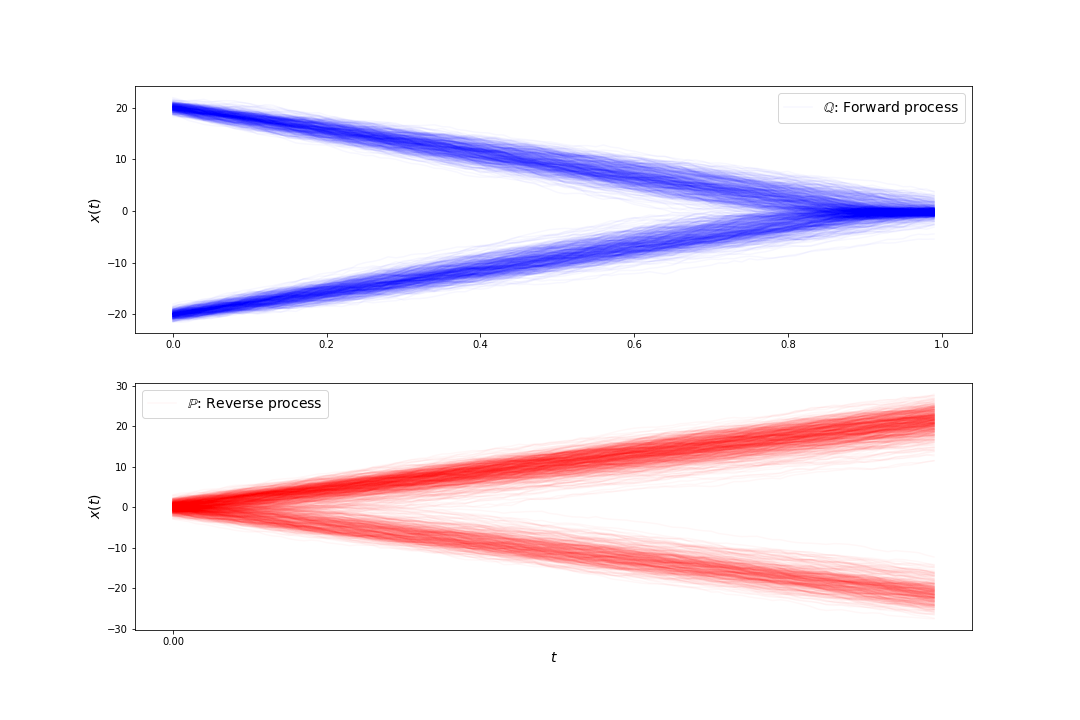
\includegraphics[scale=0.4,trim={2.3cm 1cm 2.5cm 0}, clip]{images/Control/hard_tanh_200_200__succesfl_bimodal_trajectories.png}
    \caption{ Fitted SB  trajectories using hard-tanh activation, 2 hidden layers and 200 hidden units per layer.}
    \label{fig:trajectoriesbimodtanhnnhard}
\end{figure}
\begin{figure}
    \centering
    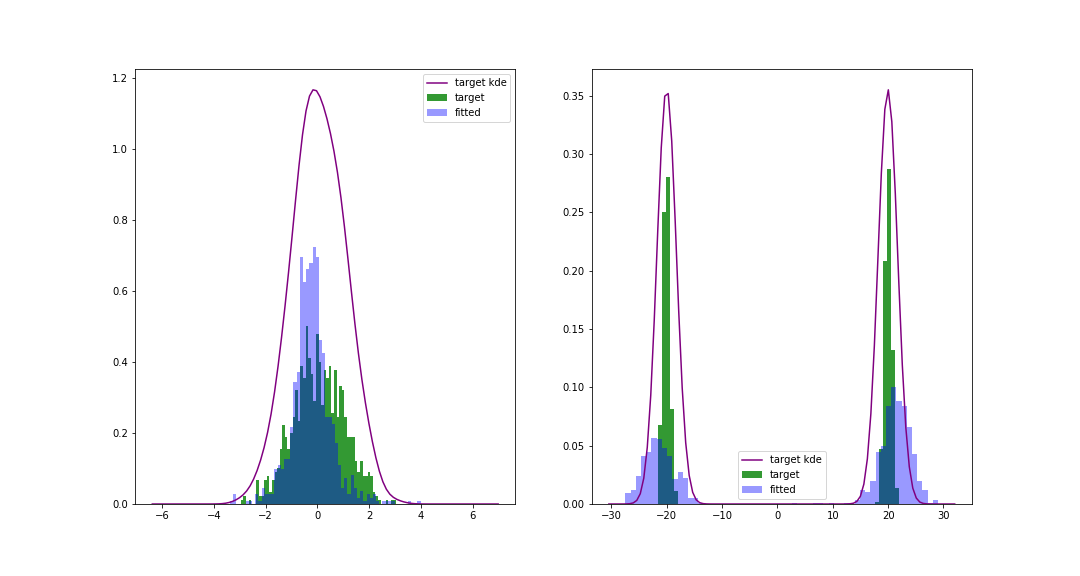
\includegraphics[scale=0.4,trim={2.3cm 1cm 2.5cm 0}, clip]{images/Control/hard_tanh_200_200_succesfl_bimodal_boundaires.png}
    \caption{ Fitted SB  boundary distributions using the SC method with hard-tanh activations, 2 hidden layers and 200 hidden units per layer.}
    \label{fig:boundsbimodtanhnnhard}
\end{figure}

As shown in Figures \ref{fig:trajectoriesbimodtanhnnhard} and \ref{fig:boundsbimodtanhnnhard}, the trajectories and results are similar to when using a tanh activation function, however the spike caused when the trajectories merge was less prominent. We believe that increasing the parameters of the network led to this improvement. Unfortunately, we were unable to improve on this issue further.  We explored several other activations, with hard-tanh giving the best results when it came to splitting.

An interesting empirical observation is that increasing the depth of the network helped with being able to split modes (which requires learning a piecewise drift), while increasing the width helped with being able to learn mappings from distributions with very different  variances. It is possible that learning drifts that are dual to each other, close to Brownian motion (close to 0) and match the boundary distributions is a very challenging task and thus reaches the maximum capacity of the neural network architectures we explored.
\subsubsection{Mode Collapse}
\begin{figure}[t]
    \centering
    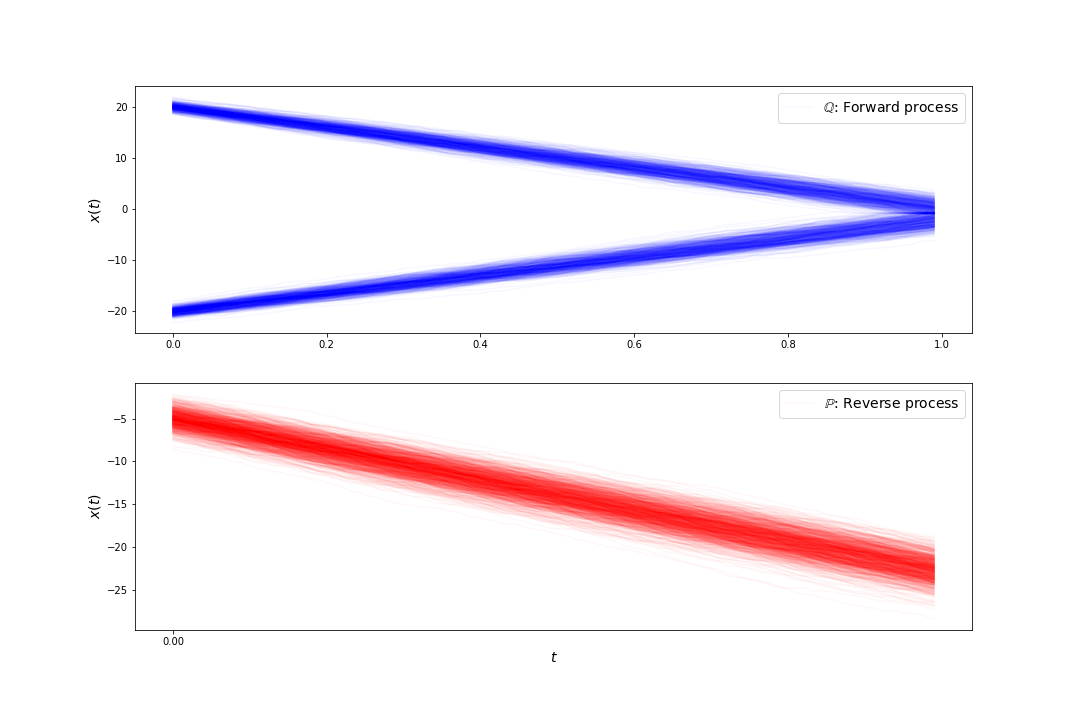
\includegraphics[scale=0.4,trim={2.3cm 1cm 2.5cm 0}, clip]{images/Control/mode_colapse_final_relu_trajectories.png}
    \caption{ Mode collapse example, using the SC method with tanh activations, 3 hidden layers 20 hidden units each.}
    \label{fig:trajectoriesmodecop}
\end{figure}
As mentioned earlier, due to minimising the reverse KL numerically, this method is in theory prone to mode collapse. In practice, mode collapse did occur fairly often, especially when the marginals were not symmetrically positioned relative to each other. 
\section{Comparison of Methods}



\begin{table}[]
\caption{Scenarios that each algorithm is able to overcome. The checkmark indicates the method can overcome this task/challenge whilst a cross indicates it is not able to do so. The exclamation mark indicates in some cases it was able to solve this milestone. The underscores indicates a lack of experiments for the relevant milestone-method pair.} \label{fig:comp_exp}
\begin{adjustbox}{width=\columnwidth}
\begin{tabular}{LlllllF}
\toprule
\multirow{3}{*}{Method} & 2 Mode                & 3 Mode                & Non                   & Small                 & Works                 & Distant            \\
                        & Split                 & Split                 & Gaussian              & variance              & at $\gamma=1$         & $\pi_0,\pi_1$              \\
                        &                       &                       & $\pi_0,\pi_1$            &                       &                       &             \\ \midrule
\cite{pavon2018data}     &\cmark &\xmark & \_                    &\xmark &\xmark &\xmark \\
Drift Estimation &\cmark &\cmark &\cmark &\xmark &\cmark &\xmark \\
Stochastic Control      &\mmark &\xmark & \_                    &\xmark &\cmark &\cmark \\
 \bottomrule
\end{tabular}
\end{adjustbox}
\end{table}


First, we summarize our findings, highlighting the empirical capacities of the three approaches we trialed. A summary of the results can be found in Table \ref{fig:comp_exp}. The main practical milestones considered when evaluating the methods are:

\begin{itemize}
    \item \textbf{ 2 Modes:} Being able to split into 2 modes and merge into 1.
    \item \textbf{ 3 Modes:} Being able to split into 3 modes and merge into one.
    \item \textbf{Non-Gaussian $\bm{\pi_0,\pi_1}$:} Being able to handle non-Gaussian boundary distributions (moons and circles datasets). 
    \item \textbf{Small Variance:} Being able to match a boundary distribution that has a numerically small variance (e.g. tending towards a point mass).  
    \item \textbf{Works at $\bm{\gamma=1}$:} Being able to work for a volatility of $\gamma=1$. We consider it working if it handles at least  a radius of 4 between the two distributions, meaning the mode that is most distant to the unimodal distribution has a magnitude of 4. The only method failing this milestone was the method by \cite{pavon2018data} since the method effectively only worked for $\gamma=1$ when the support of the data was within the unit cube.
    \item \textbf{Distant $\bm{\pi_0, \pi_1}$:} This is effectively the same milestone as above, however we do not limit the radius to 3. It tests how well the models work when the distributions are very far apart from each other. We found that the method by \cite{pavon2018data} and our direct drift estimation approach did not work well in this scenario and required either increasing $\gamma$ or standardising the data.
\end{itemize}

Inspecting the summary of findings reported Table \ref{fig:comp_exp}, we can observe that the most robust method is the direct drift estimation approach using GPs. We will now carry out a comparative experiment with a sound hypothesis test set a priori. 

\subsubsection{Comparative Results}


\begin{table}[]
\caption{Kolmogorov-Smirnov test results on learned boundary distribution. The significance level is set at $\alpha=0.05$. All methods use $\gamma=1$ with the exception of the method in \cite{pavon2018data} for which we had to use $\gamma=100$ for the Unimodal experiment.} \label{tab:final}
\begin{adjustbox}{width=\columnwidth}
\begin{tabular}{LcccccccC}
\toprule
\multirow{2}{*}{Method} & \multicolumn{4}{c}{Unimodal}                              & \multicolumn{4}{c}{Bimodal}                               \\
                        & \multicolumn{2}{c}{$\pi_0$} & \multicolumn{2}{c}{$\pi_1$} & \multicolumn{2}{c}{$\pi_0$} & \multicolumn{2}{c}{$\pi_1$} \\
                        & $D_{200}$    & $p$-value    & $D_{200}$   & $p$-value     & $D_{200}$   & $p$-value     & $D_{200}$    & $p$-value    \\ \midrule
Pavon et. al. (2018)    & $0.150$      & $0.221$      & $0.195$     & $0.001$       & $0.115$     & $0.142$       & $\bm{0.110}$      & $0.178$      \\
Direct Drift            & $\bm{0.070}$      & $0.713$      & \bm{$0.190$}     & $0.001$       & $\bm{0.110}$     & $0.178$       & $0.125$      & $0.088$      \\
Stochastic Control      & $\bm{0.070}$      & $0.713$      & $0.805$     & $< 10^{-3}$  & $0.360$     & $< 10^{-3}$  & $0.500$      & $10^{-3}$   \\ \bottomrule
\end{tabular}
\end{adjustbox}
\end{table}

In order to carry out a more quantitative comparison of the methods, we select two of the toy datasets that all methods seem to be able to fit:
\begin{align*}
\color{blue}{\pi_0(x)} &\color{blue}{= \calN(x; 0,  1)} \\
    \color{red}{\pi_1(y)} &\color{red}{= \calN(y; 4, 0.1^2)} ,
\end{align*}
and
\begin{align*}
     \color{blue}{\pi_0(x)} &\color{blue}{= \calN(x; 0,  1)} \\
    \color{red}{\pi_1(y)} &\color{red}{= \frac{1}{2}\calN(y; 1.8, 0.6 ^2)}\color{red}{ + \frac{1}{2}\calN(y; -1.9, 0.6 ^2) }.
\end{align*}
We then perform a Kolmogorov-Smirnov \citep{kolmogorov1933sulla} test where the null hypothesis is that the learned marginals from our methods are equal. We set the significance level to its usual setting  $\alpha=0.05$, meaning that if we observe a $p$-value $\leq 0.05$, we reject the null hypothesis that the two distributions are equal. We present results in Table \ref{tab:final}, displaying both the Kolmogorov test statistic as a goodness of fit measure (the lower the better) across methods and the estimated $p$-value for the test. We reject the null-hypothesis three times for the stochastic control based method meaning that it had the lowest performance across all methods. We also observe that overall the Direct Drift method and the method by \cite{pavon2018data} are fairly on-par for these two datasets.
%\chapter{Summary and Conclusions} 
\chapter{Discussion}
Schrödinger bridges have broad applications in physical sciences, but only recently have they sparked interest in the machine learning community.
In this work we have aimed to bridge this gap, firstly by trying to present an extensive yet accessible background to the problem, producing proofs for select known results whose original resource we could not find. We have highlighted some of its known connections to the more popular Wasserstein distance and thus we have suggested its potential application in machine learning as a way of comparing distributions. Furthermore, we explored the connection between IPFP and generative adversarial networks, motivating the potential application of using Schrödinger bridges for the task of domain adaptation.

We have learned and illustrated how challenging it is to develop a numerical algorithm for solving the Schrödinger bridge. Part of this challenge comes from having to deal with more than one boundary condition. This is where the g-IPFP framework comes in, allowing us to alternate between sub-problems (half bridges) with only one boundary condition until convergence. However, empirically solving these half bridges proved challenging, since they presented harder variants of typical challenges that arise in machine learning, such as numerical integration and density estimation.

We proposed two methods for solving the empirical setting of the Schrödinger bridge and explored them through simple 1D and 2D simulations which allowed us to visually and extensively evaluate the properties of the proposed methods.  We compared against the recently proposed method by \cite{pavon2018data} and showed competitive performance across two toy datasets, whilst being more robust to values of $\gamma$ than the method of \citep{pavon2018data}.

At the core of the direct drift estimation approach, we have successfully transformed a complex mathematical problem arising from the physical sciences into a classical machine learning task (regression).

\section{Summary of Contributions}

The key contributions of this thesis are:

\begin{itemize}
    \item Provided a thorough and accessible introduction to the problem, with motivational examples closer to machine learning as well as intuitive proof sketches for steps that are skipped in the available literature.
    \item Structured the existing IPFP algorithmic framework and provided formal connections between existing methods, highlighting that they are within the IPFP framework.
    \item Turned the iterative procedure for solving the Schrödinger bridge into a classical machine learning task at each iteration (i.e. regression). This contribution makes the problem much more accessible to the machine learning community.
    \item Proposed, implemented and evaluated two new working methods that use common methodology from machine learning. The newly proposed methods overcome some of the conceptual issues in \cite{pavon2018data} (e.g.\ importance sampling not scaling to high dimensions, instability for low values of $\gamma$).
    \item Using thorough experimentation, we uncovered many of the breaking points of different methods (e.g.\ mode collapse, sampling between distant boundary distributions), including ours. This is work that was missing from \cite{pavon2018data} and \cite{bernton2019schr}, thus we provided a holistic view of the methods, helpful for porting the algorithms to practical applications.
\end{itemize}

\section{Further Work}

Whilst we introduced and evaluated to a great extent the first successful machine learning based approach for solving the Schrödinger bridge, there are still areas of exploration left to pursue further:

\begin{itemize}
    \item Our best performing method is based on Gaussian processes, which will not scale well to large datasets. \cite{ruttor2013approximate} propose a sparse expectation maximisation based algorithm for inferring the drift of SDEs which we did not explore. This could potentially make the DDE method scalable enough for optimising the GP hyperparameters, which we were unable to do due to speed limitations.
    \item We found that the method by \cite{ruttor2013approximate} had difficulties in learning drifts whose end point distribution was very sharp (low variance). Optimising the hyperparameters may fix this issue.  
    \item Explore the learning of the drift using a method that is not based on Gaussian processes.
    \item Some of the unimodal examples admit closed form solutions for the full bridge. We should use this as a ground truth and compute the relative path error to the closed form drift in order to evaluate the methods.
    \item The direct half bridge drift estimation method we proposed can be adapted to the static Schrödinger bridge. This would be an interesting avenue of research, potentially reducing the computational complexity of the approach.
    \item We should explore our methods on real world data. One possible task is 2-sample hypothesis tests as in \cite{gretton2012kernel}, where we would use our approach to compare datasets to each other. 
    \item Explore and compare our proposed method with the method in \cite{bernton2019schr}.
\end{itemize}

\appendix


\singlespacing

\chapter{Analysis of simple Gaussian like Parametrisation}\label{app:bad_gauss}

This appendix illustrates the challenges in parametrising the MLE based objectives proposed in \cite{pavon2018data}, such that the partition function can be computed in closed form. Ultimately, we were unable to come up with a parametrisation that had a closed form partition function and was flexible enough to solve the half bridge for multimodal distributions.

\section{Unimodal Parametrisation}

Following the reparametrisation introduced in Section \ref{sec:unormfit}, we consider the case of parametrising the potentials with unimodal Gaussians. This allows for further analysis of the method, since both the normalisation and the updates can be attained in closed form. 

Firstly, we offer the counterexample that valid Gaussian like parametrisations for the potentials cannot solve the bridge even for unimodal Gaussian marginals:
\begin{proposition}
If we parametrise the potentials as:
\begin{align}
\hphi_0( \vx ; \beta) =  \calN(\vx | \vmu_x, \mSigma_x), \\
\phi_1( \vy ; \hat{\beta}) =  \calN(\vy | \vmu_y, \mSigma_y) ,
\end{align}
and try to solve the empirical bridge for the marginals:
\begin{align*}
    \pi_0(x) =  \mathcal{Z}_x^{-1}\calN(x,0, 1), \\
    \pi_1(y) = \mathcal{Z}_y^{-1} \calN(y,0, 10^2),
\end{align*}
then the MLE based approximation of Fortet's in \cite{pavon2018data} will not meet the marginal constraints.
\end{proposition}
\begin{proof}
 Assuming a prior $\W^{\gamma}$. Propagating:
\begin{align*}
\phi_0( \vx ; \hat{\beta}) = \mathcal{Z}_x^{-1} \calN(\vx| \vmu_y, \mSigma_y + \gamma \I),  \\
{\hphi}_1( \vy ; {\beta}) = \mathcal{Z}_y^{-1}  \calN(\vy| \vmu_x, \mSigma_x + \gamma \I).
\end{align*}
Then:
\begin{align*}
 \phi_0( \vx ; \hat{\beta})  \phi_0(\vx ; \beta) = \calN\Big(\vx \Big|& \big(\mSigma_x^{-1} + (\mSigma_y + \gamma \I)^{-1}\big)^{-1}\big( \mSigma_x^{-1}\vmu_x + (\mSigma_y + \gamma \I)^{-1}\vmu_y)\big), \\ &\big(\mSigma_x^{-1} + (\mSigma_y + \gamma \I)^{-1}\big)^{-1} \Big).
\end{align*}
Via MLE (holding $y$-parameters constant) we have:
\begin{align*}
\left(\mSigma_x^{-1} + (\mSigma_y + \gamma \I)^{-1}\right)^{-1}  = \mS_x.
\end{align*}
Yielding update
\begin{align*}
\mSigma_x^{(t)} = (\mS_x^{-1}  - (\mSigma_y^{(t-1)} + \gamma \I)^{-1})^{-1} ,
\end{align*}
and 
\begin{align*}
\left(\mSigma_x + (\mSigma_y + \gamma \I)^{-1}\right)^{-1}\left( \mSigma_x^{-1}\vmu_x + (\mSigma_y + \gamma \I)^{-1}\vmu_y)\right) = \bar{\vx}. \\
\left( \mSigma_x^{-1}\vmu_x + (\mSigma_y + \gamma \I)^{-1}\vmu_y)\right) = \left(\mSigma_x^{-1} + (\mSigma_y + \gamma \I)^{-1}\right)\bar{\vx} .
\end{align*}
Yielding update:
\begin{align*}
\vmu_x^{(i)}  = \left(\mathbb{I} + \mSigma_x^{(i)}(\mSigma_y^{(i-1)} + \gamma \I)^{-1}\right)\bar{\vx} -  \mSigma_x^{(i)}(\mSigma_y^{(i-1)} + \gamma \I)^{-1}\vmu_y^{(i-1)},
\end{align*}
and similarity  for $\mSigma_y, \vmu_y$.
In 1D (and in terms of the free parameters), the fitted marginal density variances are:
\begin{align*}
\sigma_y^{*} = \left(\frac{1}{1+\sigma^2_x} + \frac{1}{\sigma^2_y}\right)^{-1} ,\\
\sigma_x^{*} = \left(\frac{1}{1+\sigma^2_y} + \frac{1}{\sigma^2_x}\right)^{-1}.
\end{align*}
If the empirical marginal variances were $1,10$:
\begin{align*}
1 = \left(\frac{1}{1+\sigma^2_x} + \frac{1}{\sigma^2_y}\right)^{-1}, \\
10 = \left(\frac{1}{1+\sigma^2_y} + \frac{1}{\sigma^2_x}\right)^{-1}.
\end{align*}
Then the above system has no valid solutions (can be solved only for negative values of $\sigma_x$), by the quadratic formula:
\begin{align*}
0.8 \sigma_x^4 + 1.9 \sigma_x^2 + 1 = 0. \quad \quad \quad \text{\Lightning}
\end{align*}

\end{proof}

The above tells us that in order to do a squared exponential paremetrisation for the potentials, we must drop the positive definite constraint. In geometric terms, if one potential is log concave then the other needs to be log convex due to how the variances combine.

We must still enforce an integrability constraint (required to make the inner product of potentials converge):
\begin{align*}
\left(\mSigma_x^{-1} +\mSigma_y^{-1}\right)^{-1} = \mL\mL^{\top},
\end{align*}
which implies:
\begin{align*}
\mSigma_x^{-1} +\mSigma_y^{-1} = \mL\mL^{\top},
\end{align*}
which can be enforced via a simple reparametrisation (this allows for negative lengthscales):
\begin{align*}
\mSigma_x = (\mL\mL^{\top} -\mSigma_y^{-1})^{-1},
\end{align*}
where $\mL$ can be parametrised in terms of an unconstrained vector.
\section{Mixture of Exponentiated Quadratics}


We now consider whether it is possible to extend the exponentiated quadratic  parametrisation of the potentials to a mixture of exponentiated quadratics. In order to achieve this parametrisation, we need to reconsider the integrability constraint.

\begin{align}
\hphi_0( \vx ; \beta) =  \sum_{k_x} \pi_{k_x} \calN(\vx | \vmu_{k_x}, \mSigma_{k_x}) \\
\phi_1( \vy ; \hat{\beta}) = \sum_{k_y} \pi_{k_y}  \calN(\vy | \vmu_{k_y}, \mSigma_{k_y}) 
\end{align}
The integrability constraint then becomes $\forall k_x$:
\begin{align*}
   \bigwedge_{k_y} \left(\mSigma_{k_x} +\mSigma_{k_y} \succ 0\right), 
\end{align*}

which using the eigen-decompositions $\mSigma_{k_x}=\mU_{k_x} \mD_{k_x} \mU^{\top}_{k_x}$,  $\mSigma_{k_y}=\mU_{k_y} \mD_{k_y} \mU^{\top}_{k_y}$ can be re-expressed as: 
\begin{align*}
  \lambda_{k_x}^d + \min\lambda_{k_y}^d \geq 0,
\end{align*}
where $d$ is a specific component / dimension. Thus, we enforce this constraint via the reparametrisation:
\begin{align*}
   \lambda_{k_x}^d = \exp(\theta) - \min\lambda_{k_y}^d ,
\end{align*}
where  $\theta$ is unconstrained. Furthermore, we can parametrise the orthogonal matrices $\mU_{k_x}$ in terms of unconstrained vectors using Householder reflections. Combining the aforementioned parametrisations, we can enforce the integrability constraint fully via reparametrisations. While these parametrisations are not differentiable everywhere, one can still maximise the liklelihood using the sub-gradient method \citep{shor1991development}. Unfortunately, this method was unable to work for multimodal distributions, thus we did not pursue this path further.



\bibliographystyle{icml} 
\bibliography{bibliography}                                                                                         

\end{document}
